\immediate\write18{makeindex -g -s ../Templates/Arbeit.ist TeXAux/Skript.idx}
\immediate\write18{cat TeXAux/Skript.nlo | sort | uniq -w 55 | makeindex -i -s nomencl.ist -o TeXAux/Skript.nls}
\immediate\write18{cd TeXAux;gnuplot *.gnuplot;cd ..;}

\documentclass[twoside, a4paper]{article}
\usepackage{beamerarticle}
\pdfminorversion=6

% Projekt-Definitionen
\newcommand{\GetItDigitalModulnumber}{1}
\newcommand{\GetItDigitalModulname}{Elektrische Grundgrößen}
\newcommand{\GetItDigitalAutoren}{Henrik Bode}
\newcommand{\GetItDigitalAutorenListe}{H. Bode}
\newcommand{\GetItDigitalLink}{https://getitdigital.uni-wuppertal.de/module/modul-1-elektrische-grundgroessen}
					% Modulspezifische Settings einbinden


\usepackage[utf8]{inputenc}         % Zeichenkodierung auf UTF-8
\usepackage[ngerman]{babel}         % Deutsche Texte, Sonderzeichen
\usepackage{color, colortbl}		% Farben, Tabellenfarben
\usepackage{multirow}			   	% Tabellen
\usepackage{booktabs}				% better tables (\toprule, \midrule, \bottomrule)
\usepackage{ifthen}                 % Konditionen
\usepackage{makeidx}                % automatische Index-Generierung
\usepackage[german]{nomencl}        % Nomenklatur (Symbolverzeichnis)
\usepackage{etoolbox}               % Gliederung von der Nomenklatur
\usepackage{icomma}				    % kein Leerzeichen hinter einem Komma, wenn es in einer Zahl steht
\usepackage{amsmath}                % Mathematische Symbole
\usepackage{amsfonts}               % Mathematische Symbole
\usepackage{amssymb}                % Mathematische Symbole
\usepackage{mathtools}				% Addon for amsmath (z.B. für \mathclap)
\usepackage{cancel}				    % Durchstreichen von Formelteilen
\usepackage{textcomp, gensymb}	    % Grad-Zeichen
\usepackage{xargs}					% Eigene Kommandos mit optionalen Argumenten definieren \newcommandx* für eigenes \highlight command basierend auf hf-tikz
\usepackage{booktabs}	   			% Für schönere horizontale Linien (FH Aachen)
\usepackage[intlimits]{esint}		% Schönere Integrale
\usepackage{siunitx}	   			% Für SI-Einheiten (FH Aachen)
\usepackage{colortbl}	   			% Farben (FH Aachen)
\usepackage{subcaption}             % Für Unterabbildungen (FH Aachen)
%\usepackage{caption}                % Caption (FH Aachen)
\usepackage[nice]{nicefrac}			% Math fracs in nice!
\usepackage{xfrac}					% newer than nicefrac \sfrac{}{} > \nicefrac{}{}
\usepackage{bm}						% Hervorhebung von Teilen einer Formel

% float-Positionierungen:
\usepackage{float}  			    % Gleitobjekte mit H genau an die angegebene Stelle positionieren.
\usepackage{placeins} 			    % neuer Befehl: \FloatBarrier  zu dem Zeitpunkt werden alle Floats gesetzt.

% Schaltpläne und LaTeX-Grafiken
\usepackage[nosiunitx,european,straightvoltages]{circuitikz}
\usepackage{tikz}
\usepackage{siunitx}
\usepackage{pgfplots}			    % Bode Diagramme
\usepackage{mathrsfs}				% Laplace Zeichen
%tabellen damit schaltungen ausgerrichtet sind
\usepackage{array}
\setlength{\marginparwidth}{2cm}	%Eingefügt von Jonas, um die To-Dos richtig darzustellen

%Lernziele, Merksätze und Beispiele
\usepackage{varwidth}
\usepackage[most,skins,breakable]{tcolorbox}
% Grid Overlay zur Positionierungshilfe - DEBUGGING ONLY
%\usepackage[texcoord,grid,gridcolor=red!60,subgridcolor=green!60,gridunit=mm]{eso-pic}
\usepackage{graphicx}				% for subfigures and resizeboxtikz
\usepackage{adjustbox}[export]		% crop images relative to image width/height
\usepackage{tcolorbox}				% Farbige Boxen für Definitionen, Beispiele etc.
\tcbuselibrary{skins}
\tcbuselibrary{breakable}			% für Seitenumbrüche in tcolorbox
%\usepackage{varwidth}

\usepackage{svg}					%Einbindung von svg-Grafiken

\usepackage{overpic}	                            % Text auf Bild platzieren

\usepackage{silence}                                        % Suppress warnings with \WarningFilter
\WarningFilter{latex}{You have requested package}           % Suppress warning about package location
\usepackage{../Templates/beamervideo}                       % Videoerstellung

% Optionen des Grafikpakets TikZ
\usetikzlibrary{arrows}				% schönere Pfeilspitzen
\usetikzlibrary{datavisualization}
\usetikzlibrary{angles}				% Winkelberechnung und Darstellung
\usetikzlibrary{decorations.markings}
\usetikzlibrary{patterns}           % gefüllte Flächen
\usetikzlibrary{shapes.geometric}	% Geometrische Formen (z.B. Dreieck für Verstärker)
\usepgfplotslibrary{fillbetween}	% Fläche zwischen zwei Kurven
\tikzset{>=stealth'}				% schönere Pfeilspitzen

% Bilder in getrenntem Pfad:
\graphicspath{{Bilder/}{../Templates/Bilder/}}


% eigene Befehle
\newcommand{\red}[1]{\textcolor[rgb]{1.00,0.00,0.00}{#1}}
\newcommand{\blue}[1]{\textcolor[rgb]{0.00,0.00,1.00}{#1}}
\newcommand{\Hz}{\operatorname{Hz}} % für gerades Hz
\newcommand{\dB}{\operatorname{dB}} % für gerades dB (Dezibel)
\newcommand{\dBm}{\operatorname{dBm}} % für gerades dBm {Dezibel auf 1 mW bezogen}
\renewcommand{\Re}{\operatorname{Re}} % für gerades Re für Realteil wie in physics package (statt Fraktur-R wie in plain TeX)
\renewcommand{\Im}{\operatorname{Im}} % für gerades Im für Imaginärteil wie in phycis package (statt Fraktur-I wie in plain TeX)
\newcommand{\dt}[1][{}]{\frac{\mathrm{d}^{#1}}{\mathrm{d}t^{#1}}} % \dt = d/dt ; \dt[2] = d^2/dt^2
% Note: \Re, \Im in Superscript/Subscript immer mit {}, Bsp. ^{\Im} oder _{\Re} statt ^\Im oder _\Re damit beide styles funktionieren
\newcommand{\alttexxt}[1]{} % Alternativtext für Bilder. Wird zur Zeit noch ignoeriert.

% Durchstreichen von Formelteilen
\definecolor{Red}{rgb}{1,0,0}
\newcommand{\colorcancel}[2]{\renewcommand{\CancelColor}{\color{#2}}\cancel{#1}}	% \colorcancel{text to cancel}{color}
\newcommand{\redcancel}[2][red]{\renewcommand{\CancelColor}{\color{#1}}\cancel{#2}} % \redcancel[optional color]{text to cancel} <=compatible=> \cancel{text to cancel}

% Multi Footnotes (gleiche Nummer, gleicher Text)
\newcommand{\footm}{\footnotemark} %https://tex.stackexchange.com/questions/86650/how-to-display-the-footnote-in-the-bottom-of-the-slide-while-using-columns
\newcommand*{\footmc}[1][0]{\addtocounter{footnote}{#1}\footnotemark[\value{footnote}]{}}% footmark with either same number (default) or by optional argument incremented number
\newcommand{\foott}[1]{\footnotetext{#1}}
% 	blabla\footm         ... undso\footmc\\ % 1...1
% 	blabla\footmc[-1]    ... undso\footmc\\ % 2...2
%	blabla\footmc[-1]    ... undso\footmc 	% 3...3
%	\foott{1st info} \foott{2nd info} \foott{3rd info}	 % footnotetexts
\newcommand\CMT[1]\null% Intra-Line Comments à la \CMT{this is a comment} https://www.reddit.com/r/LaTeX/comments/1cmq3v/intraline_comments_comment_without_commenting_out/

% Symbole für Stern- und Dreieckschaltung
\newcommand{\Stern}{{\ifmmode%
		\text{\tikz \draw[] (0,0) -- (90:.9ex) -- (0,0) -- (-45:1.1ex) -- (0,0) -- (225:1.1ex);}%
		\else%
		\tikz \draw[] (0,0) -- (90:.9ex) -- (0,0) -- (-45:1.1ex) -- (0,0) -- (225:1.1ex);%
		\fi}}
\newcommand{\Dreieck}{{\ifmmode%
		\text{\tikz \draw[] (0,0) -- (65:1.5ex) --++ (-65:1.5ex) --cycle;}%
		\else%
		\tikz \draw[] (0,0) -- (65:1.5ex) --++ (-65:1.5ex) --cycle;%
		\fi}}

% Farbige Spannungs und Strompfeile
% Ref: Circuitikz Manual, Kapitel Advanced voltages, currents and flows https://texdoc.org/serve/circuitikz/0#subsection.5.8 (v. 1.6.7)
\ctikzset{bipole voltage style/.style={color=voltage}} % voltage label color
\ctikzset{bipole current style/.style={color=red}} 	% current label color
\ctikzset{!vi/.style={no v symbols, no i symbols}}	% add option for argument "!vi" to remove voltage and current arrows
\ctikzset{!v/.style={no v symbols}}	% add option for argument "!v" to remove voltage arrows
\ctikzset{!i/.style={no i symbols}}	% add option for argument "!i" to remove current arrows

\newcommand{\varronly}[1]{% {node}
	\draw [color=voltage] (#1-Vfrom) .. controls (#1-Vcont1) and (#1-Vcont2) .. (#1-Vto) node [currarrow, sloped, anchor=tip, allow upside down, pos=1]{} % arrow
}
\newcommand{\iarronly}[1]{% {node}
	%\draw [red, -] (#1-Ifrom) -- (#1-Ipos); % arrow shaft (optional)
	\node [color=red, currarrow, anchor=center,	rotate=\ctikzgetdirection{#1-Iarrow}] at (#1-Ipos) {} % arrow tip
}

% modified versions of above commands to draw arrows and labels together in one command with optional color argument
\newcommand{\varrmore}[3][voltage]{% [color]{node}{label}
    \draw[color=#1] (#2-Vfrom) .. controls (#2-Vcont1) and (#2-Vcont2) .. (#2-Vto) node [currarrow, sloped, anchor=tip, allow upside down, pos=1]{}; % arrow
    \node[color=#1, anchor=\ctikzgetanchor{#2}{Vlab}, inner sep=2pt] at (#2-Vlab) {#3} % label
	% note: label offset [...,inner sep=2pt] copied from internal macro definition, s. /usr/share/texlive/texmf-dist/tex/latex/circuitikz/circuitikz-1.2.7-body.tex line 23009)
}
\newcommand{\iarrmore}[3][red]{% [color]{node}{label}
	%\draw[#1,-] (#2-Ifrom) -- (#2-Ipos); % arrow shaft (optional)
	\node[color=#1, currarrow, anchor=center, rotate=\ctikzgetdirection{#2-Iarrow}] at (#2-Ipos) {}; % arrow tip
	\node[color=#1, anchor=\ctikzgetanchor{#2}{Ilab}] at (#2-Ipos) {#3} % label
}



% logarithmische Achsen für den Bode-Plot
\pgfplotsset{
	compat=1.18,
	log x ticks with fixed point/.style={
		xticklabel={
			\pgfkeys{/pgf/fpu=true}
			\pgfmathparse{exp(\tick)}%
			\pgfmathprintnumber[fixed relative, precision=3]{\pgfmathresult}
			\pgfkeys{/pgf/fpu=false}
		}
	},
	log y ticks with fixed point/.style={
		yticklabel={
			\pgfkeys{/pgf/fpu=true}{\tiny }
			\pgfmathparse{exp(\tick)}%
			\pgfmathprintnumber[fixed relative, precision=3]{\pgfmathresult}
			\pgfkeys{/pgf/fpu=false}
		}
	}
}


% Für minipage, weil \columns nur in Beamer funktioniert
\newlength\Colsep
\setlength\Colsep{10pt}

% Für hf-tikz, Offsets to adjust vertical bounds highlight boxes for typical equation sizes
%\usepackage{xparse} % needed for hf-tikz
\def\hfoffupper{0.3} 	% e.g. for 1
\def\hfoffuppera{0.45} 	% e.g. for \frac{1}{1}
\def\hfoffupperb{0.7}	% e.g. for \frac{\frac{\int^1_0 11}{\int^1_0 12}}{\frac{\int^1_0 21}{\int^1_0 22}}
\def\hfoffupperc{0.9}
\def\hfofflower{-0.12}	% analog zu upper offset
\def\hfofflowera{-0.21}
\def\hfofflowerb{-0.55}
\def\hfofflowerc{-0.7}

%Farbdefinitionen
\definecolor{GETgreen}{RGB}{25,185,145}				%Titelstreifen der Folien
\definecolor{leiter}{RGB}{207,163,118}				%elektrischer Leiter
\definecolor{magnetfeld}{RGB}{255,128,0}			%magnetisches Feld
\definecolor{flaeche}{RGB}{121,179,205}				%Querschnittsfläche
\definecolor{voltage}{RGB}{26, 91, 144}				%Spannungspfeile
\definecolor{spannung}{RGB}{26, 91, 144}			%farbe für spannung definieren
\definecolor{current}{RGB}{200, 0, 0}				%Strompfeile
\definecolor{strom}{RGB}{200, 0, 0}					%farbe für strom definieren
\definecolor{durchflutung}{RGB}{25, 210, 220}		%magnetiche Durchflutung Theta
\definecolor{Red}{rgb}{255, 0, 0}					%Reines rot z.B. zum durchstreichen von Elementen die sich wegkürzen
\definecolor{plotgreen}{RGB}{0,200,0}				% green
\definecolor{green1}{RGB}{0,200,0}					% green
\definecolor{magnetfeld}{RGB}{255,128,0}
\definecolor{statorw1}{RGB}{230,103,35}
\definecolor{statorw2}{RGB}{169,82,0}
\definecolor{statorw3}{RGB}{215,25,0}

%Farbkommandos für Gleichungen (equation color)
% usage: \ec[optional color]{mathsymbols} for any color or e.g. \ecg{mathsymbols} for green mathsymbols
% ref: https://tex.stackexchange.com/questions/21598/how-to-color-math-symbols
\newcommand{\ec}[2][black]{{\color{#1}#2}}	% set text/equation coloring, default black
\newcommand{\eci}[1]{{\color{red}#1}}		% current color
\newcommand{\ecv}[1]{{\color{voltage}#1}} 	% voltage color
\newcommand{\ecr}[1]{{\color{red}#1}} 		% red color
\newcommand{\ecg}[1]{{\color{green}#1}} 	% green color
\newcommand{\ecb}[1]{{\color{blue}#1}} 		% blue color
\newcommand{\ecp}[1]{{\color{purple}#1}} 	% purple color
\newcommand{\ecy}[1]{{\color{yellow}#1}} 	% yellow color
\newcommand{\ecc}[1]{{\color{cyan}#1}} 		% cyan color
\newcommand{\eco}[1]{{\color{orange}#1}} 	% orange color

%Lernziel
\newtcolorbox{Lernziele}[1]{enhanced,
	before skip=1cm,
	after skip=1cm,
	colframe=GETgreen,
	colbacktitle=GETgreen,
	colback=white!95!black,
	boxrule=0.5mm,
	title={Lernziele: #1},
	attach boxed title to top left={xshift=1.14cm,yshift*=-\tcboxedtitleheight/2}, varwidth boxed title*=-3cm,
	boxed title style={
		frame code={
			\path[left color=tcbcolback,right color=tcbcolback,
				middle color=tcbcolback]
				([xshift=1.6mm]frame.north west)[rounded corners=0.5mm]
				-- ([xshift=1.6mm]frame.north east)
				-- ([xshift=-1mm]frame.south east)
				-- ([xshift=-1mm]frame.south west)
				-- cycle;
			\path[left color=tcbcolback,right color=tcbcolback,
				middle color=tcbcolback]
				([xshift=-3mm]frame.north west)[rounded corners=0.5mm]
				-- ([xshift=0.3mm]frame.north west)
				-- ([xshift=-2.2mm]frame.south west)
				-- ([xshift=-5.5mm]frame.south west)
				-- cycle;
			\path[left color=tcbcolback,right color=tcbcolback,
				middle color=tcbcolback]
				([xshift=-7.6mm]frame.north west)[rounded corners=0.5mm]
				-- ([xshift=-4.3mm]frame.north west)
				-- ([xshift=-6.8mm]frame.south west)
				-- ([xshift=-10.1mm]frame.south west)
				-- cycle;
		},interior engine=empty,
	},fonttitle=\bfseries
}

%Merksatz
\newtcolorbox{Merksatz}[1]{enhanced,
	before skip=1cm,
	after skip=1cm,
	colframe=GETgreen,
	colbacktitle=GETgreen,
	colback=GETgreen!5!white,
	boxrule=0.5mm,
	title={Merke: #1},
	attach boxed title to top left={xshift=1.14cm,yshift*=-\tcboxedtitleheight/2}, varwidth boxed title*=-3cm,
	boxed title style={
		frame code={
			\path[left color=tcbcolback,right color=tcbcolback,
				middle color=tcbcolback]
				([xshift=1.6mm]frame.north west)[rounded corners=0.5mm]
				-- ([xshift=1.6mm]frame.north east)
				-- ([xshift=-1mm]frame.south east)
				-- ([xshift=-1mm]frame.south west)
				-- cycle;
			\path[left color=tcbcolback,right color=tcbcolback,
				middle color=tcbcolback]
				([xshift=-3mm]frame.north west)[rounded corners=0.5mm]
				-- ([xshift=0.3mm]frame.north west)
				-- ([xshift=-2.2mm]frame.south west)
				-- ([xshift=-5.5mm]frame.south west)
				-- cycle;
			\path[left color=tcbcolback,right color=tcbcolback,
				middle color=tcbcolback]
				([xshift=-7.6mm]frame.north west)[rounded corners=0.5mm]
				-- ([xshift=-4.3mm]frame.north west)
				-- ([xshift=-6.8mm]frame.south west)
				-- ([xshift=-10.1mm]frame.south west)
				-- cycle;
		},interior engine=empty,
	},fonttitle=\bfseries
}


% logarithmische Achsen für den Bode-Plot
\pgfplotsset{
	compat=1.18,
	log x ticks with fixed point/.style={
		xticklabel={
			\pgfkeys{/pgf/fpu=true}
			\pgfmathparse{exp(\tick)}%
			\pgfmathprintnumber[fixed relative, precision=3]{\pgfmathresult}
			\pgfkeys{/pgf/fpu=false}
		}
	},
	log y ticks with fixed point/.style={
		yticklabel={
			\pgfkeys{/pgf/fpu=true}{\tiny }
			\pgfmathparse{exp(\tick)}%
			\pgfmathprintnumber[fixed relative, precision=3]{\pgfmathresult}
			\pgfkeys{/pgf/fpu=false}
		}
	}
}


% Farbige Spannungs und Strompfeile
% Ref: Circuitikz Manual, Kapitel Advanced voltages, currents and flows https://texdoc.org/serve/circuitikz/0#subsection.5.8 (v. 1.6.7)
\ctikzset{!vi/.style={no v symbols, no i symbols}}  		% add option for argument "!vi" to remove voltage and current arrows

%Tabellenbefehle
\usepackage{ragged2e}
\newcolumntype{L}[1]{>{\raggedright\arraybackslash}p{#1}}
\newcolumntype{C}[1]{>{\centering\arraybackslash}p{#1}}
\newcolumntype{R}[1]{>{\raggedleft\arraybackslash}p{#1}}
\newcolumntype{J}[1]{>{\justifying\arraybackslash}p{#1}}
	 		% Allgemeine Settings einbinden
% Pakete nur für das Skript
\usepackage{fancyhdr}      		% Unterstrichene Kopfzeilen: selbstdefinierbar
\usepackage{sanitize-umlaut}	   % Umlaute im Index
\usepackage[pdftex,bookmarks,bookmarksopen=false,colorlinks,bookmarksnumbered]{hyperref} % Links im PDF anklickbar
\hypersetup{% \ref Links im Skript umfärben
    ,urlcolor=blue
    ,citecolor=blue
    ,linkcolor=blue
    }
\usepackage{hf-tikz}		                        % Highlighting Text/Math, Ref: https://tex.stackexchange.com/questions/52598/beamer-highlighting-aligned-math-with-overlay
% example1: \tikzmarkin<2->[above offset={\hfoffuppera},below offset={\hfofflowera},blend mode=multiply]{a} R = \frac{U}{I} \tikzmarkend{a}
% example2: \tikzmarkin<2-3>[above left offset={0,\hfoffuppera}, below right offset={0,\hfofflowera}]{markerid} \int^{\pi}_{0}f(x)\d x \tikzmarkend{markerid}
% option: blend mode=multiply (to not overshadow stuff behind the highlight box) and (in beamer mode) <n>, <n->, <n-m> for overlay (ignored in article)

\usepackage{enumitem} % Aufzählungen nummerisch oder alphabetisch
\usepackage{todonotes}	%Anmerkungen und to-dos erstellen
	 	% Allgemeine Foliensettings einbinden
\usepackage[disabled]{../Video/beamervideo}  % Videoerstellung deaktiviert

%PDF Eigenschaften
\hypersetup{
	pdftitle={GET it digital},
	pdfsubject={Modul \GetItDigitalModulnumber: \GetItDigitalModulname},
	pdfauthor={\GetItDigitalAutorenListe}
}

\title{Modul \GetItDigitalModulnumber: \GetItDigitalModulname}
\author{}
\institute{GET it digital}
\date{\today}

\begin{document}

\thispagestyle{empty}
\begin{center}

	\begin{minipage}[c][2cm][c]{0.3\textwidth}
		
\includegraphics[angle=270,width=\linewidth]{FHAachen-logo2010}
	\end{minipage}
	\hfill
	\begin{minipage}[c][2cm][c]{0.3\textwidth}
		
\includegraphics[width=\linewidth]{Logo_Uni_Paderborn}
	\end{minipage}
	\hfill
	\begin{minipage}[c][2cm][c]{0.3\textwidth}
		
\includegraphics[width=\linewidth]{BUW_Logo-weiss-auf-gruen-rgb}
	\end{minipage}
	\\
	\begin{minipage}[c][2cm][c]{0.3\textwidth}
		\includegraphics[width=\linewidth]{Fachhochschule_Südwestfalen_logo}
	\end{minipage}
	\hfill
	\begin{minipage}[c][2cm][c]{0.3\textwidth}
		
\includegraphics[width=\linewidth]{logo-hrw}
	\end{minipage}
	\hfill
	\begin{minipage}[c][2cm][c]{0.3\textwidth}
		\begin{center}
			
\includegraphics[width=0.7\linewidth]{FH_Dortmund-logo}
		\end{center}
	\end{minipage}

	\vfill
	\vspace{23ex}
	{{\large GET it digital} \\[10ex]
		\large Modul \GetItDigitalModulnumber:\\[0.5ex]}
	{\huge \GetItDigitalModulname\\[20ex]}

	{\large
		\GetItDigitalAutoren
	}
\end{center}
\vfill

\begin{minipage}[t]{0.36\textwidth}
	Ein Kooperationsvorhaben \\
	empfohlen durch die\\[0.3cm]
	
\includegraphics[width=\linewidth]{dh_nrw.jpg}
\end{minipage}
\hfill
\begin{minipage}[t]{0.5\textwidth}
	gefördert durch\\[1cm]
	
\includegraphics[width=\linewidth]{mkw.jpg}
\end{minipage}



\newpage
\pagestyle{fancyplain}
\ \\
\vfill
{\hfill Stand: \today}\\
{
\includegraphics[width=0.2\linewidth]{by.png}}\\
Weiternutzung als OER ausdrücklich erlaubt: Dieses Werk und dessen Inhalte sind lizenziert unter CC BY 4.0. Ausgenommen von der Lizenz
sind die verwendeten Logos sowie alle anders gekennzeichneten Elemente. Nennung gemäß \href{https://open-educational-resources.de/oer-tullu-regel/}{TULLU-Regel} bitte wie folgt: \glqq GET it digital Modul \GetItDigitalModulnumber: \GetItDigitalModulname\grqq\ von \GetItDigitalAutorenListe \ Lizenz: CC BY 4.0.

Der Lizenzvertrag ist hier abrufbar:\\
\url{https://creativecommons.org/licenses/by/4.0/deed.de}\\
Das Werk ist online verfügbar unter:\\
\url{\GetItDigitalLink}
\newpage
	% Titelseite

{\setlength{\parskip}{0.05ex}    %Verringerter Zeilenabstand für Verzeichnisse
	\tableofcontents
	\newpage
}

\printnomenclature
\cleardoublepage

\pagestyle{fancyplain}
\pagenumbering{arabic}
\setheadkapitel

\cleardoublepage



\newvideofile{Einleitung}{Grundlagen elektrischer Netzwerke}


\s{
\section{Einleitung}

Elektrische Netzwerke sind in der heutigen Welt omnipräsent. Sie bestehen aus Zusammenschaltungen 
von verschiedenen elektrischen Bauteilen, welche durch Verbindungsleitungen miteinander
 verknüpft sind. In der Realität kommen sie in den verschiedensten Funktionen und Größenordnungen vor. 
So kann ein elektrisches Netzwerk sowohl eine kleine elektronische Schaltung innerhalb eines Mikrocontrolers
mit einer Größe von einigen Mikrometern darstellen, als auch ein elektrisches Energieverteilungsnetz 
mit Ausdehnungen von bis zu einigen 1000 Kilometern abbilden, wie sie symbolisch in den Abbildungen \ref{fig:platine} bzw. \ref{fig:stromnetz} angedeutet sind. 




\begin{frame} 
	\begin{minipage}{0.45\textwidth}

		\f{width=\textwidth}{width=0.7\textwidth}{netzklein.png}{Symbolbild eines kleinen elektrischen Netzwerkes auf einer Platine  \label{fig:platine}}
	%	\fo{width=\textwidth}{width=\textwidth}{Magnetisches_Feld_Leiter}{
		%	\put(60.5, 9){\color{red}$I$}
	%	}{{\bf Magnetisches Feld um einen stromdurchflossenen Leiter.} Die Rich\-tung des Feldes kann mit der \glqq Rechten-Hand-Regel\grqq\ veranschaulicht werden.}
	\end{minipage}
	\hfill\pause
	\begin{minipage}{0.45\textwidth}

		\f{width=\textwidth}{width=0.7\textwidth}{netzgross.png}{Symbolbild eines großen elektrischen Netzwerkes  \label{fig:stromnetz}}
	%	\fo{width=\textwidth}{width=\textwidth}{Magnetisches_Feld_Leiterschleife}{
		%	\put(31.5, 18){\color{red}$I$}
		%	\put(65, 4){\color{red}$I$}
		%	\put(5, 37){\color{magnetfeld}N}
		%	\put(80, 79){\color{magnetfeld}S}
	%	}{{\bf Magnetisches Feld um eine stromdurchflossene, geöffnete Lei\-ter\-schleife.} Die Leiterschleife stellt die klein\-ste Einheit einer Spule dar.}
	\end{minipage}
\end{frame}

\vspace{10pt}

Dieses Kapitel bietet eine Einführung zu grundlegenden Berechnungen in elektrischen Gleichstromnetzwerken.
Ziel dieser Berechnung ist es in der Regel, die Spannungen und Ströme in allen Bauteilen des Netzwerkes
 zu berechnen. Reale Bauteile werden dazu in der Regel vereinfacht als Kombination idealer Zweipole dargestellt
  (Beispiele: Tabelle \ref{tab:schaltzeichen}). Aus der Verschaltung dieser 
  Zweipole lässt sich ein vereinfachtes Modell der realen Schaltung aufbauen, welches das grundlegende Verhalten der 
  Schaltung nachbildet.
  Dieses Modell bildet die Grundlage zur mathematischen Berechnung der Schaltung.

 
 Da in diesem Kapitel ausschließlich lineare Bauteile wie Widerstände oder ideale Gleichspannungsquellen verwendet werden, ist eine analytische 
 Berechnung grundsätzlich immer möglich. In fortgeschrittenen Modulen werden hingegen nichtlineare Bauelemente
 wie reale Operationsverstärker oder Dioden eingeführt. In diesem Fall ist oft eine iterative bzw. numerische Herangehensweise
 notwendig.



}





\begin{frame}

	\b{
		\fta{Elektrische Netzwerke}

	\begin{columns}
		\column[t]{0.5\textwidth}

		Elektrische Netzwerke bestehen aus: 
		\begin{itemize}
			\item Zwei- oder Mehrpolen: Elemente mit zwei oder mehreren el. Anschlüssen
			\item Verbunden durch ideal leitende Verbindungen
		\end{itemize}

		\phantom{.}\\

		Diese können zu Systemen unterschiedlichster Größen geschaltet werden:
		
		\begin{itemize}
			\item Energieverteilnetze \>1000 km Ausdehnung
			\item Elektronische Schaltungen im Mikrometerbereich (Mikrocontroler)
		\end{itemize}


		
	
		\column[t]{0.5\textwidth}

		\f{width=\textwidth}{width=0.7\textwidth}{netzgross.png}{Symbolbild eines kleinen elektrischen Netzwerkes auf einer Platine}
		\begin{center}
			Symbolbilder
		\end{center}

		\f{width=\textwidth}{width=0.7\textwidth}{netzklein.png}{Symbolbild eines kleinen elektrischen Netzwerkes auf einer Platine}

	\end{columns}
	\speech{elektrische_netzwerke}{1}{, Elektrische Netzwerke sind heute überall verbaut – in unseren Smartphones, Computern oder im riesigen Stromnetz, das ganze Städte versorgt.
Aber was genau ist ein elektrisches Netzwerk?
Im Grunde ist es eine Verbindung verschiedener elektrischer Bauteile über Leitungen. Diese Bauteile, wie Widerstände, Kondensatoren oder Halbleiter, übernehmen unterschiedliche Aufgaben.
Grundsätzlich bestehen elektrische Netzwerke aus sogenannten Zwei- oder Mehrpolen – also Bauteilen mit zwei oder mehr Anschlüssen. Über diese Anschlüsse werden sie miteinander verbunden, und zwar über ideale Leitungen. Diese Leitungen haben – theoretisch – keinen eigenen Widerstand und übertragen den Strom verlustfrei.
Elektrische Netzwerke gibt es in allen Größenordnungen:
Winzige Schaltungen in Mikrocontrollern, kaum größer als ein Staubkorn,
bis hin zu riesigen Energieverteilungsnetzen, die sich über tausende Kilometer erstrecken und unseren Strom liefern.}



	}
\end{frame}	






%\begin{frame}
%	\fta{Elektrische Netzwerke}
%	\s{Während bisher die Behandlung von von wichtigen Grundbegriffen im Fokus stand, wird ab jetzt die Anwendung dieser auf Einfache Schaltungen im Vordergrund stehen.}
%	\begin{columns}
%	\column[t]{0.5\textwidth}
%	\begin{center}
%	%Motivation Zweipole: Können zu Netzwerk verschaltet werden, 
%	%wie teilen sich Strom/Spannung auf als offene Frage.
%	Ziel: Berechnung der auftretenden Größen in einer elektrischen Schaltung
%	\begin{itemize}
%		\item Vereinfachung der realen Bauteile zu idealen \textbf{Zweipolen} (Bauteile mit zwei Anschlüssen)
%		\item Darstellung der Zweipole durch Ersatzschaltbilder (siehe Tabelle)
%		\item Modellierung (Verschaltung) der idealen Zweipole zu \textbf{Netzwerken}
%		\item Modell stellt grundlegendes Verhalten der realen elektrischen Schaltung dar
%		\item vereinfachtes Modell bildet Grundlage zur mathematischen Berechnung
%	\end{itemize}
%	\end{center}
%	\column[t]{0.5\textwidth}
%	\f{width=\textwidth}{width=\textwidth}{Uebersicht_Ersatzschaltbilder.png}{Übersicht relevanter Ersatzschaltbilder}
%	Muss noch nachgebaut werden!
%	\end{columns}
%\end{frame}

%\begin{frame}
%	\fta{Elektrische Netzwerke}
%	\begin{columns}
%	\column[t]{0.5\textwidth}
%
%	Ziel: Berechnung der auftretenden Größen in einer elektrischen Schaltung
%	\begin{itemize}
%		\item Vereinfachung der realen Bauteile zu idealen Zweipolen
%		\item Darstellung der Zweipole durch Ersatzschaltbilder (siehe Tabelle)
%		\item Modellierung (Verschaltung) der idealen Zweipole
%		\item Modell stellt grundlegendes Verhalten der realen elektrischen Schaltung dar
%		\item vereinfachtes Modell bildet Grundlage zur mathematischen Berechnung
%	\end{itemize}
%	Wie teilen sich Strom und Spannung in einem Netzwerk auf?
%	\column[t]{0.5\textwidth}
%
%	Beispiele für Zweipole:
%
%
%	\begin{center}
%		\begin{tabular}{|c|c|}
%		\hline
%		Bauelement & Schaltzeichen \\
%		\hline
%		%Spannungsquelle &  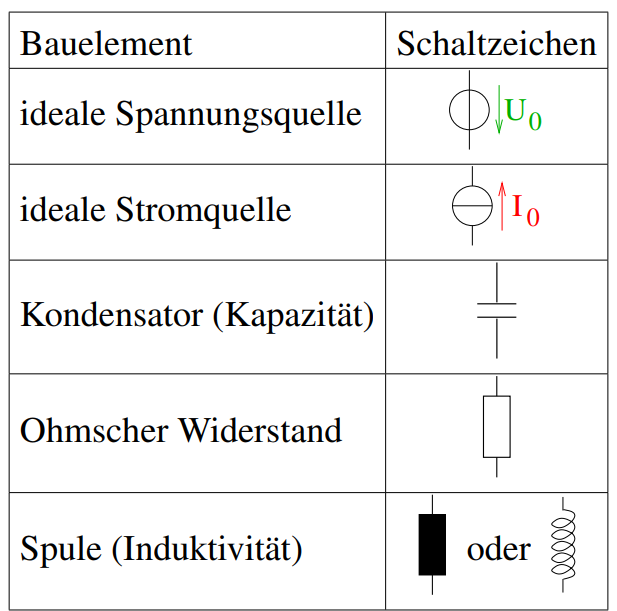
\includegraphics{Uebersicht_Ersatzschaltbilder.png} \\
%		ideale Spannungsquelle & {\begin{circuitikz} \draw(0,1.5) to[european voltage source=$U_{\mathrm{0}}$] (0,0); \end{circuitikz}} \\
%		\hline
%		ideale Stromquelle & {\begin{circuitikz} \draw(0,0) to[european current source=$I_{\mathrm{0}}$] (0,1.5); \end{circuitikz}} \\
%		\hline
%		Kondensator (Kapazität) & {\begin{circuitikz} \draw(0,0) to[C] (1.5,0); \end{circuitikz}} \\
%		\hline
%		Ohmescher Widerstand & {\begin{circuitikz} \draw(0,0) to[R] (1.5,0); \end{circuitikz}} \\
%		\hline
%		Spule (Induktivität) & {\begin{circuitikz} \draw(0,0) to[L] (1.5,0); \end{circuitikz}}  \\
%		\hline
%	\end{tabular}
%	\end{center}
%	\end{columns}
%\end{frame}

\begin{frame}

	\b{
	\ftx{Elektrische Netzwerke}
	\begin{columns}
	\column[t]{0.45\textwidth}

	Ziel: Berechnung der elektrischen Größen in einer Schaltung

	\vspace{5pt}
	\begin{itemize}
		\item Vereinfachung der realen Bauteile zu idealen Zweipolen
		\item Darstellung der Zweipole durch Ersatzschaltbilder (siehe Tabelle)\\
		$\rightarrow$ bilden Grundlage zur mathematischen Berechnung		
		\item Ersatzschaltbild modelliert grundlegendes Verhalten der realen elektrischen Schaltung
		
	\end{itemize}
	
	\column[t]{0.55\textwidth}

	Beispiele für Zweipole:



	


	\begin{center}
		\begin{tabular}{|c|c|}
		\hline
		Zweipol & Schaltzeichen \\
		\hline
		%Spannungsquelle &  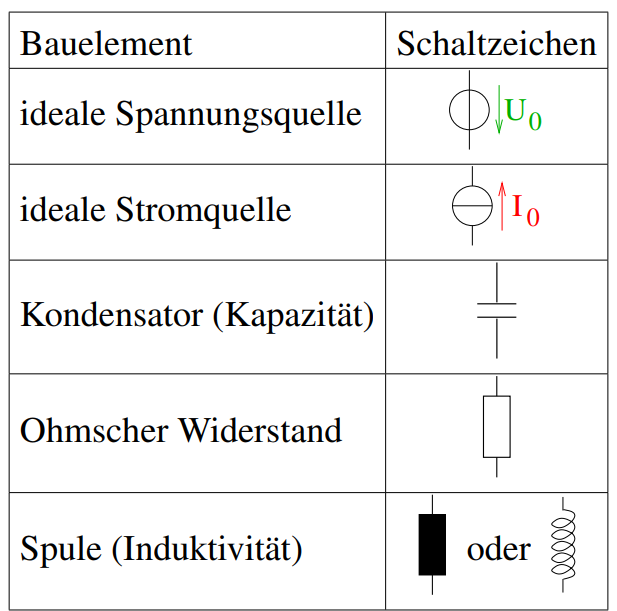
\includegraphics{Uebersicht_Ersatzschaltbilder.png} \\
		%ideale Spannungsquelle
		\begin{tikzpicture}[x=1mm,y=1mm]\draw[draw=none] (-10,-7) rectangle (+10,+7); \node[draw=none,align=center] {ideale Spannungsquelle};\end{tikzpicture} & {\begin{tikzpicture} \draw(0,1.5) to[european voltage source, name=V] (0,0); \draw[white] (-1.3,1.5) to[] (-1.35,1.59); \varrmore{V}{$U_0$}; \end{tikzpicture}} \\
		\hline
		\begin{tikzpicture}[x=1mm,y=1mm]\draw[draw=none] (-10,-7) rectangle (+10,+7); \node[draw=none,align=center] {ideale Stromquelle};\end{tikzpicture} & {\begin{tikzpicture} \draw(0,0) to[european current source, name=A] (0,1.5); \iarrmore{A}{$I_0$}; \end{tikzpicture}} \\
		\hline
		\begin{tikzpicture}[x=1mm,y=1mm]\draw[draw=none] (-10,-2) rectangle (+10,+2); \node[draw=none,align=center] {Kondensator (Kapazität)};\end{tikzpicture} & {\begin{tikzpicture} \draw(0,0) to[C] (1.5,0); \draw[white] (-0.1,-.10) to[] (0,0.5);\end{tikzpicture}} \\
		\hline
		\begin{tikzpicture}[x=1mm,y=1mm]\draw[draw=none] (-10,-2) rectangle (+10,+2); \node[draw=none,align=center] {Ohmscher Widerstand};\end{tikzpicture}& {\begin{tikzpicture} \draw(0,0) to[R] (1.5,0);  \draw[white] (-0.1,-.10) to[] (0,0.35); \end{tikzpicture}} \\
		\hline
		\begin{tikzpicture}[x=1mm,y=1mm]\draw[draw=none] (-10,-1) rectangle (+10,+4); \node[draw=none,align=center] {Spule (Induktivität)};\end{tikzpicture}& {\begin{tikzpicture} \draw(0,0) to[L] (1.5,0); \draw[white] (-0.1,-.10) to[] (0,0.35); \end{tikzpicture}}  \\
		\hline
	\end{tabular}
	\end{center}
	\end{columns}


\speech{folie4}{1}{Auf den folgenden Folien dieses Kapitel steigen wir in die grundlegenden Berechnungen von elektrischen Gleichstromnetzwerken ein.
Doch was ist das eigentliche Ziel der abstrakten, mathematischen Betrachtungsweise realer Netzwerke?
Wir wollen herausfinden, welche Spannungen und Ströme an den einzelnen Bauteilen im Netzwerk auftreten.
Um diese Berechnungen überhaupt durchführen zu können, vereinfachen wir reale Bauteile.
Diese werden als Kombination aus idealen Zweipolen dargestellt, Beispiele dafür findet ihr in der nebenstehenden Tabelle.
Durch diese Vereinfachung entsteht ein Modell der Schaltung, das sich gut berechnen lässt, aber trotzdem das grundlegende Verhalten des echten Netzwerks abbildet.
Dieses Modell bildet dann die Basis für unsere mathematischen Berechnungen.
In diesem Kapitel verwenden wir ausschließlich lineare Bauteile, wie Widerstände und ideale Gleichspannungsquellen.
Das hat einen großen Vorteil:
Die Schaltungen lassen sich analytisch, also mathematisch exakt, berechnen.}


	}
\end{frame}

\newpage

\section{Zweipole und Zählpfeilsysteme}



\begin{frame}{}
	\ftx{Lernziele: Zweipole und Zählpfeilsysteme}

	\begin{Lernziele}{Zweipole und Zählpfeilsysteme}
        Die Studierenden können
        \begin{itemize}
            \item den Begriff des Zweipols erläutern sowie gängige Zweipole nennen und deren Schaltsymbole verwenden
            \item das Erzeuger- sowie Verbraucherzählpfeilsystem erläutern und entsprechend der Konventionen anwenden
			\item die zentralen Elemente des Grundstromkreises erläutern und die Zusammenhänge zwischen diesen erkennen
        \end{itemize}
    \end{Lernziele}

	\speech{folie5}{1}{Hier also nochmal zusammengefasst die Lernziele dieser Einheit:
Nach dieser Lektion könnt ihr,
den Begriff des Zweipols erklären, typische Zweipole benennen und ihre Schaltsymbole sicher verwenden,
das Erzeuger- und Verbraucherzählpfeilsystem erläutern und korrekt nach den Konventionen anwenden,
und ihr könnt die zentralen Elemente eines Grundstromkreises beschreiben und die Zusammenhänge zwischen ihnen verstehen.}


	
\end{frame}




\begin{frame}
	\ftb{Zweipole}


	\s{Als Zweipol (Abb. \ref{fig:zweipol}) wird ein Bauelement mit zwei äußeren Anschlussklemmen bezeichnet. Der innere Aufbau dieser
	Zweipole kann dabei von gänzlich unterschiedlicher Art und Komplexität sein. Beispielsweise ist ein einfacher
	elektrischer Widerstand, aber auch eine Spannungsquelle (beispielsweise eine Autobatterie) oder ein Haartrockner
	 (sofern dieser nur zwei Anschlussleitungen besitzt) als Zweipol zu sehen.
	Bauteile mit mehr Anschlussleitungen werden entsprechend als Dreipol (z.B. Kühlschrank mit Schutzleiter), 
	Vierpol (z.B. Transformator) oder gar Fünfpol (elektrischer Herd mit Drehstromanschluss, Schutzleiter und Neutralleiter) bezeichnet.

	Unabhängig von der inneren Komplexität kann ein Zweipol im elektrischen Netzwerk vollständig durch die Beziehung von Strom
	und Spannung an seinen Anschlusspunkten, dem sogenannten \textbf{Klemmenverhalten}, charakterisiert werden. 
	Zu beachten ist dabei, dass der in Abbildung \ref{fig:zweipol} eingezeichnete Strom $I_1$ eines Zweipols stets genauso groß wie der Strom $I_2$ ist.

	Die praktische Realisierung der Bauteile wie reale Baumaße, Materialeigenschaften, parasitäre Effekte oder interne
	inhomogene Feldstärkeverteilungen
	werden in der Netzwerkberechnung mit Zweipolen vernachlässigt.

	\begin{figure}[h!]
		\begin{center}
			\begin{tikzpicture}
    
				\draw (0,0) rectangle (1.5,1.5);
			
				\draw (1.5, 1.25) to[short,i<, name=in, -o] (2.3, 1.25) node[right] {};
				\draw (1.5, 0.25) to[short,i, name=out, -o] (2.3, 0.25) node[right] {};
			
				\draw[white] (2.6, 1.5) to[short,v>, name=volti] (2.6, 0.0) node[right] {};

				\varrmore{volti}{$U$};			
				\iarrmore{in}{$I_1$};
				\iarrmore{out}{$I_2$};
				
			\end{tikzpicture}
			
		\end{center}
		\caption{Allgemeine Darstellung eines Zweipols mit den gleich großen Stromstärken $I_1$ und $I_2$ sowie der anliegender Spannung $U$}
		\label{fig:zweipol}
	\end{figure}


	Einige der bereits aus vorherigen Kapiteln bekannte Zweipole sind in Tabelle \ref{tab:schaltzeichen} beispielhaft aufgeführt.







\begin{center}
	\begin{table}[h!]
		\centering
		\begin{tabular}{|c|c|}
			\hline
			Zweipol & Schaltzeichen \\
			\hline
			%Spannungsquelle &  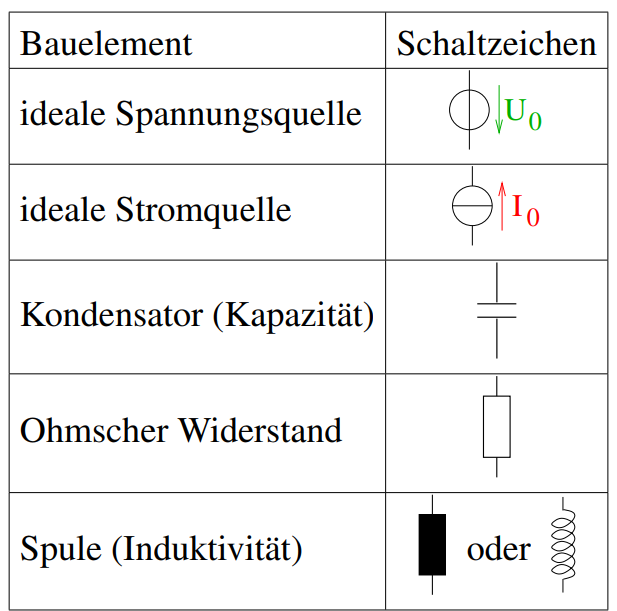
\includegraphics{Uebersicht_Ersatzschaltbilder.png} \\
			%ideale Spannungsquelle
			\begin{tikzpicture}[x=1mm,y=1mm]\draw[draw=none] (-10,-7) rectangle (+10,+7); \node[draw=none,align=center] {ideale Spannungsquelle};\end{tikzpicture} & {\begin{tikzpicture} \draw(0,1.5) to[european voltage source, name=V] (0,0); \draw[white] (-1.3,1.5) to[] (-1.35,1.59); \varrmore{V}{$U_0$}; \end{tikzpicture}} \\
			\hline
			\begin{tikzpicture}[x=1mm,y=1mm]\draw[draw=none] (-10,-7) rectangle (+10,+7); \node[draw=none,align=center] {ideale Stromquelle};\end{tikzpicture} & {\begin{tikzpicture} \draw(0,0) to[european current source, name=A] (0,1.5); \iarrmore{A}{$I_0$}; \end{tikzpicture}} \\
			\hline
			\begin{tikzpicture}[x=1mm,y=1mm]\draw[draw=none] (-10,-2) rectangle (+10,+2); \node[draw=none,align=center] {Kondensator (Kapazität)};\end{tikzpicture} & {\begin{tikzpicture} \draw(0,0) to[C] (1.5,0); \draw[white] (-0.1,-.10) to[] (0,0.5);\end{tikzpicture}} \\
			\hline
			\begin{tikzpicture}[x=1mm,y=1mm]\draw[draw=none] (-10,-2) rectangle (+10,+2); \node[draw=none,align=center] {Ohmscher Widerstand};\end{tikzpicture}& {\begin{tikzpicture} \draw(0,0) to[R] (1.5,0);  \draw[white] (-0.1,-.10) to[] (0,0.35); \end{tikzpicture}} \\
			\hline
			\begin{tikzpicture}[x=1mm,y=1mm]\draw[draw=none] (-10,-1) rectangle (+10,+4); \node[draw=none,align=center] {Spule (Induktivität)};\end{tikzpicture}& {\begin{tikzpicture} \draw(0,0) to[L] (1.5,0); \draw[white] (-0.1,-.10) to[] (0,0.35); \end{tikzpicture}}  \\
			\hline
		\end{tabular}
		\caption{Beispiele verschiedener Zweipole sowie ihrer Schaltzeichen}
		\label{tab:schaltzeichen}
	\end{table}
\end{center}










	}



	\b{

	\begin{columns}
		\column[t]{0.7\textwidth}

Allgemein:\\
\phantom{.}\\
\begin{itemize}
	\item Zwei äußere Anschlüsse
	\item Klemmströme $I_1$ und $I_2$ sind gleich groß ($I_1=I_2 = I$)
	\item Klemmverhalten (Verhältnis von $I$ und $U$)
	\item Reale Baumaße, Materialeigenschaften, Feldstärkenverteilung im Bauteil werden vernachlässigt
\end{itemize}

 




\column[t]{0.3\textwidth}

\vspace{10pt}







\begin{tikzpicture}
    
    \draw (0,0) rectangle (1.5,1.5);



    \draw (1.5, 1.25) to[short,i<, name=in, -o] (2.3, 1.25) node[right] {};
    \draw (1.5, 0.25) to[short,i, name=out, -o] (2.3, 0.25) node[right] {};

	\draw[white] (2.6, 1.5) to[short,v>, name=volti] (2.6, 0.0) node[right] {};
	\varrmore{volti}{$U$};

	
	\iarrmore{in}{$I_1$};
	\iarrmore{out}{$I_2$};


    
\end{tikzpicture}

\end{columns}

\phantom{text}\\



	\textbf{Aktiver Zweiphl}: enthält Strom/Spannungsquelle(n) und ggfs. Widerstände, Kondensatoren, Spulen...\\


	\textbf{Passiver Zweipol}: Enthält keine Quellen, sondern ausschließlich Widerstände, Kondensatoren, Spulen...

\begin{columns}
	\column[t]{0.6\textwidth}



	\column[t]{0.4\textwidth}
\end{columns}

\speech{folie6}{1}{Schauen wir uns jetzt genauer an, was ein Zweipol eigentlich ist.
Ein Zweipol, wie rechts dargestellt, ist ein Bauelement mit genau zwei äußeren Anschlussklemmen.
Wie komplex der innere Aufbau dieses Bauteils ist, spielt dabei erstmal keine Rolle.
Ein einfacher Widerstand kann ein Zweipol sein, genau wie eine Spannungsquelle, etwa eine Autobatterie, oder sogar ein Haartrockner, solange er nur zwei Anschlussleitungen hat.
Wichtig ist:
Unabhängig von der inneren Komplexität reicht es in der Netzwerkanalyse aus, das sogenannte Klemmenverhalten zu betrachten, also die Beziehung zwischen Strom und Spannung an den Anschlussklemmen.
Ein Punkt, den ihr euch unbedingt merken solltet:
Der Strom, der in einen Zweipol hingeht, ist immer genauso groß wie der Strom, der auf der anderen Seite wieder herauskommt. Als Analogie könnt ihr euch hier einen Gartenschlauch vorstellen, das gesamte Wasser, das auf der einen Seite in den Schlauch geht, verlässt diesen auch wieder auf der anderen Seite.
Zusätzlich unterscheiden wir zwischen aktiven und passiven Zweipolen:
Ein aktiver Zweipol enthält mindestens eine Strom- oder Spannungsquelle, eventuell auch Widerstände, Kondensatoren oder Spulen.
Ein passiver Zweipol dagegen enthält keine Quellen, sondern ausschließlich passive Bauelemente wie Widerstände, Kondensatoren oder Spulen.
Und noch etwas:
In unseren Berechnungen vernachlässigen wir praktische Details wie die genauen Baumaße, Materialeigenschaften oder parasitäre Effekte innerhalb des Bauteils.
Das macht die Analyse deutlich einfacher, und trotzdem ausreichend genau für unsere Zwecke.}

}
\end{frame}


\subsection{Zählpfeilsysteme}




\begin{frame}
	\ftx{Zählpfeilsysteme}

	\s{
 
	Die Wahl der Zählrichtungen von Strom und Spannung ist grundsätzlich beliebig. Bei der Berechnung
	elektrischer Netzwerke wird häufig versucht, die Zählrichtungen so einzuführen, dass die
	Ströme und Spannungen positiv sind. Das ist für von vornherein bekannte Größen durchaus
	sinnvoll. Für unbekannte Größen muss die Zählrichtung hingegen willkürlich festgelegt werden. Es wird
	dadurch nicht ausgedrückt, dass der Strom tatsächlich in der Pfeilrichtung fließt bzw. eine
	positive Spannung in Pfeilrichtung anliegt. Die tatsächliche Richtung wird dann durch das
	Vorzeichen der Spannung ausgedrückt.
	Für eine vorzeichengerechte Beschreibung von Strömen und Spannungen ist also eine
	Bemaßung mit Zählpfeilen zwingend notwendig.

	Bei Zweipolen wird zwischen den in Tabelle \ref{tab:zps} vorgestellten zwei unterschiedlichen Zählpfeilsystemen unterschieden:


	\begin{Merksatz}{Verbraucher- und Erzeugerzählpfeilsysteme}
	
		\textbf{Verbraucher-Zählpfeilsytem (VPS)}: Strom und Spannung werden am Zweipol gleichsinnig gezählt. Anzuwenden bei passiven Zweipolen (z.B. Widerständen)\\
		
		\textbf{Erzeuger-Zählpfeilsystem (EPS)}: Strom und Spannung werden am Zweipol entgegengesetzt gezählt. Anzuwendn bei aktiven Zweipolen (z.B. Spannungsquellen)

	\end{Merksatz}


	\begin{table}[h!]
		\centering
		\begin{tabular}{|c|c|c|c|}
			\hline
			Zählpfeilsystem & Erzeugte Leistung & Verbrauchte Leistung & Zählpfeile am Verbraucher \\ \hline
			\begin{tikzpicture}[x=1mm,y=1mm]\draw[draw=none] (-10,-10) rectangle (+10,+10); \node[draw=none,align=center] {VPS}; \end{tikzpicture} & \begin{tikzpicture}[x=1mm,y=1mm]\draw[draw=none] (-10,-10) rectangle (+10,+10); \node[draw=none,align=center] {\( P = -UI \) }; \end{tikzpicture} & \begin{tikzpicture}[x=1mm,y=1mm]\draw[draw=none] (-10,-10) rectangle (+10,+10); \node[draw=none,align=center] {\( P = UI > 0 \)}; \end{tikzpicture}  &
				\begin{tikzpicture}	
					\draw[white] (-0.5, 1.6) to[short,v>] (2, 1.6) node[right] {};		
					\draw[white] (-0.8, 0.05) to[short,v>, name=volti] (2.3, 0.05) node[right] {};		
					\draw (0,0) rectangle (1.5,1.5);
				
					\draw (-0.8, 0.75) to[short,i, name=in, o-] (0, 0.75) node[right] {};
					\draw (1.5, 0.75) to[short,i, name=out, -o] (2.3, 0.75) node[right] {};
					
					\varrmore{volti}{$U$};			
					\iarrmore{in}{$I$};
				
				\end{tikzpicture} \\ \hline
	%		\begin{tikzpicture}		
	%				\draw (0,0) rectangle (1.5,1.5);
	%			
	%				\draw (1.5, 1.25) to[short,i<, name=in, -o] (2.3, 1.25) node[right] {};
	%				\draw (1.5, 0.25) to[short,i, name=out, -o] (2.3, 0.25) node[right] {};
	%			
	%				\draw[white] (2.6, 1.5) to[short,v>, name=volti] (2.6, 0.0) node[right] {};
	%
	%				\varrmore{volti}{$U$};			
	%				\iarrmore{in}{$I_1$};
					%\iarrmore{out}{$I_1$};
				
	%		\end{tikzpicture} \\ \hline
	\begin{tikzpicture}[x=1mm,y=1mm]\draw[draw=none] (-10,-10) rectangle (+10,+10); \node[draw=none,align=center] {EPS}; \end{tikzpicture} & \begin{tikzpicture}[x=1mm,y=1mm]\draw[draw=none] (-10,-10) rectangle (+10,+10); \node[draw=none,align=center] {\( P = UI > 0 \)}; \end{tikzpicture}  & \begin{tikzpicture}[x=1mm,y=1mm]\draw[draw=none] (-10,-10) rectangle (+10,+10); \node[draw=none,align=center] {\( P = -UI \)}; \end{tikzpicture} &



			\begin{tikzpicture}	
				\draw[white] (-0.5, 1.6) to[short,v>] (2, 1.6) node[right] {};		
				\draw[white] (-0.8, 0.05) to[short,v>, name=volti] (2.3, 0.05) node[right] {};		
				\draw (0,0) rectangle (1.5,1.5);
			
				\draw (-0.8, 0.75) to[short,i<, name=in, o-] (0, 0.75) node[right] {};
				\draw (1.5, 0.75) to[short,i, name=out, -o] (2.3, 0.75) node[right] {};
				
				\varrmore{volti}{$U$};			
				\iarrmore{in}{$I$};
			
			\end{tikzpicture} \\ \hline


			%\begin{tikzpicture}
	%			\draw (0,0) rectangle (1.5,1.5);
	%			
	%			\draw (1.5, 1.25) to[short,i, name=in, -o] (2.3, 1.25) node[right] {};
	%			\draw (1.5, 0.25) to[short,i<, name=out, -o] (2.3, 0.25) node[right] {};
	%		
	%			\draw[white] (2.6, 1.5) to[short,v>, name=volti] (2.6, 0.0) node[right] {};
%
%				\varrmore{volti}{$U$};			
%				\iarrmore{in}{$I$};
				%\iarrmore{out}{$I_1$};
%			\end{tikzpicture} \\ \hline
		\end{tabular}
		\caption{Vergleich zwischen Verbraucherzählpfeilsystem (VPS) und Erzeugerzählpfeilsystem (EPS)}
		\label{tab:zps}
	\end{table}





	\begin{Merksatz}{Zählpfeile}
		Zählpfeile dienen der Zählweise und sind nicht mit Vektoren zu verwechseln!
	\end{Merksatz}

	}

	

	\b{
	Zählpfeilrichtung theoretisch beliebig, jedoch Konventionen: 
	\begin{itemize}
		\item Verbraucher-Zählpfeilsytem (VPS): Strom und Spannung \textbf{gleichsinnig}\\
		 (passive Zweipole, z.B. Widerständen)
		\item Erzeuger-Zählpfeilsystem (EPS): Strom und Spannung \textbf{entgegengesetzt}\\
		 (aktive Zweipole, z.B. Spannungsquellen)
	\end{itemize}



	\begin{table}[h!]
		\centering
		\begin{tabular}{|c|c|c|c|}
			\hline
			Zählpfeilsystem & Erzeugte Leistung & Verbrauchte Leistung & Zählpfeile am Verbraucher \\ \hline
			\begin{tikzpicture}[x=1mm,y=1mm]\draw[draw=none] (-10,-10) rectangle (+10,+10); \node[draw=none,align=center] {VPS};\end{tikzpicture} &
			\begin{tikzpicture}[x=1mm,y=1mm]\draw[draw=none] (-10,-10) rectangle (+10,+10); \node[draw=none,align=center] {\( P = -UI < 0 \)};\end{tikzpicture} &  
			\begin{tikzpicture}[x=1mm,y=1mm]\draw[draw=none] (-10,-10) rectangle (+10,+10); \node[draw=none,align=center] {\( P = UI > 0 \)};\end{tikzpicture} &
			\begin{tikzpicture}	
				\draw[white] (-0.5, 1.6) to[short,v>] (2, 1.6) node[right] {};		
				\draw[white] (-0.8, 0.05) to[short,v>, name=volti] (2.3, 0.05) node[right] {};		
				\draw (0,0) rectangle (1.5,1.5);
			
				\draw (-0.8, 0.75) to[short,i, name=in, o-] (0, 0.75) node[right] {};
				\draw (1.5, 0.75) to[short,i, name=out, -o] (2.3, 0.75) node[right] {};
				
				\varrmore{volti}{$U$};			
				\iarrmore{in}{$I$};
			
			\end{tikzpicture} \\ \hline
	
	%		\begin{tikzpicture}		
	%				\draw (0,0) rectangle (1.5,1.5);
	%			
	%				\draw (1.5, 1.25) to[short,i<, name=in, -o] (2.3, 1.25) node[right] {};
	%				\draw (1.5, 0.25) to[short,i, name=out, -o] (2.3, 0.25) node[right] {};
	%			
	%				\draw[white] (2.6, 1.5) to[short,v>, name=volti] (2.6, 0.0) node[right] {};
	%
	%				\varrmore{volti}{$U$};			
	%				\iarrmore{in}{$I$};
	%				%\iarrmore{out}{$I_1$};
	%			
	%		\end{tikzpicture} \\ \hline
			\begin{tikzpicture}[x=1mm,y=1mm]\draw[draw=none] (-10,-10) rectangle (+10,+10); \node[draw=none,align=center] {EPS};\end{tikzpicture} &  
			\begin{tikzpicture}[x=1mm,y=1mm]\draw[draw=none] (-10,-10) rectangle (+10,+10); \node[draw=none,align=center] {\( P = UI > 0 \)};\end{tikzpicture} & 
			\begin{tikzpicture}[x=1mm,y=1mm]\draw[draw=none] (-10,-10) rectangle (+10,+10); \node[draw=none,align=center] {\( P = -UI < 0 \)};\end{tikzpicture} &
			\begin{tikzpicture}	
				\draw[white] (-0.5, 1.6) to[short,v>] (2, 1.6) node[right] {};		
				\draw[white] (-0.8, 0.05) to[short,v>, name=volti] (2.3, 0.05) node[right] {};		
				\draw (0,0) rectangle (1.5,1.5);
			
				\draw (-0.8, 0.75) to[short,i<, name=in, o-] (0, 0.75) node[right] {};
				\draw (1.5, 0.75) to[short,i, name=out, -o] (2.3, 0.75) node[right] {};
				
				\varrmore{volti}{$U$};			
				\iarrmore{in}{$I$};
			
			\end{tikzpicture} \\ \hline
	
	
			%		\begin{tikzpicture}
	%			\draw (0,0) rectangle (1.5,1.5);
				
	%			\draw (1.5, 1.25) to[short,i, name=in, -o] (2.3, 1.25) node[right] {};
	%			\draw (1.5, 0.25) to[short,i<, name=out, -o] (2.3, 0.25) node[right] {};
			
	%			\draw[white] (2.6, 1.5) to[short,v>, name=volti] (2.6, 0.0) node[right] {};

	%			\varrmore{volti}{$U$};			
	%			\iarrmore{in}{$I$};
				%\iarrmore{out}{$I_1$};
	%		\end{tikzpicture} \\ \hline
		\end{tabular}
		
	\end{table}

	\speech{folie7}{1}{ Mit diesen Grundlagen können wir jetzt die Wahl der Zählrichtungen für Strom und Spannung betrachten. Als Zählpfeil werden die in Pfeile bezeichnet, die dem Strom beziehungsweise der Spannung zugeordnet werden. Wir brauchen Zählpfeile, damit unsere Berechnungen eindeutig sind.

Grundsätzlich ist es erstmal beliebig, in welche Richtung wir Ströme und Spannungen ansetzen.
In der Praxis wählen wir die Zählrichtungen aber oft so, dass die Ergebnisse möglichst positive Werte liefern – wenn wir die Richtung schon kennen.
Kennen wir sie noch nicht, müssen wir die Richtung willkürlich festlegen.
Ob unsere Annahme stimmt, zeigt sich später:,
Ein positives Ergebnis bestätigt die Richtung,
ein negatives Ergebnis bedeutet, dass der Strom oder die Spannung entgegen unserer Vorgabe fließt.
Bei Zweipolen gibt es dafür zwei wichtige Zählpfeilsystem (formal in der untenstehenden Tabelle zu sehen):
Das Verbraucher-Zählpfeilsystem, oft VPS abgekürzt: Strom und Spannung zeigen in dieselbe Richtung, dies wird typischerweise für Widerstände und andere passive Bauteile.
Beim Erzeuger-Zählpfeilsystem oder auch EPS zeigen Strom und Spannung in dei entgegengesetzte Richtung, dieses wird oft typi bei Spannungsquellen und andere aktive Bauteile verwendet.
Anzumerken ist jedoch folgendes:
Zählpfeile sind keine Vektoren! Sie legen nur die Zählrichtung fest, nicht eine physikalische Richtung im Raum.
}


	}

\end{frame}





%\begin{frame}
%	\fta{Elektrische Netzwerke}
%
%	\begin{columns}
%		\column[c]{0.5\textwidth}
%		Die wichtigsten Begriffe sind in der Abbildung dargestellt:
%		\begin{itemize}
%			\item idealsierte Zweipole bilden \textbf{Zweige} des Netzwerks
%			\item Verbindung der einzelnen Zweige über \textbf{Konten}
%			\item geschlossene Kette von Zweigen bildet \textbf{Masche}
%		\end{itemize}
%		Wie teilen sich Strom und Spannung in einem Netzwerk auf?
%		\column[c]{0.5\textwidth}
%		\begin{circuitikz}
%           \draw(0,0) to[R=$R_\mathrm{1}$] (0,2)
%			to[R=$R_{\mathrm{2}}$] (3,2)
%           to[V=$U_{\mathrm{0}}$,-*] (3,0)
%            to[short,-*](0,0);
%			\draw(3,0) to[R=$R_\mathrm{3}$] (3,-2)
%			to[short](0,-2)
%			to[R=$R_{\mathrm{4}}$] (0,0);
%			\draw[dashed](-0.9,-0.25) to[short] (-0.9,-2.5)
%			to[short] (3.9,-2.5)
%			to[short] (3.9,-0.25)
%			to[short] (2.5,-0.25)
%			to[short] (2.5,-1.5)
%			to[short] (0.5,-1.5)
%			to[short] (0.5,-0.25)
%			to[short] (-0.9,-0.25);
%			\draw
%			(1.5,-4.2)
%			node[label={above:$Zweig$}] {};
%			\draw
%			(4.0,0)
%			node[label={right:$Knoten$}] {};
%			\draw[->,shift={(1.5,0.6)}] (180:.8cm) arc (180:0:.8cm) node at(0,0){$Masche$};
%			\draw[->] (4,0) -- (3.2,0);
%			\draw[->] (1.5,-3.5) -- (1.5,-2.6);
%       \end{circuitikz}
%	 \end{columns}
%\end{frame}

\begin{frame}
	\ftx{Der Grundstromkreis}

	\subsection{Der Grundstromkreis}
	\s{

	Die zuvor eingeführten Zweipole (oder auch Mehrpole) lassen sich zu einem 
	elektrischen Netzwerk zusammenschließen.\\


	\begin{figure}[h!]
		\begin{center}

     	\begin{tikzpicture}
		\only<1-3>{\draw(0,0) to[R=$R_1$] (0,2)
		to[R=$R_2$] (3,2)
		to[V,v,name=V,-*] (3,0)
		to[short,-*](0,0);}
		\draw(3,0) to[R=$R_3$] (3,-2)
		to[short](0,-2)
		to[R=$R_4$] (0,0);
		\only<2->{\draw[dashed, draw = teal](-0.9,-0.25) to[short] (-0.9,-2.5)
		to[short] (3.9,-2.5)
		to[short] (3.9,-0.25)
		to[short] (2.5,-0.25)
		to[short] (2.5,-1.5)
		to[short] (0.5,-1.5)
		to[short] (0.5,-0.25)
		to[short] (-0.9,-0.25);
		\draw(1.5,-4.2)node[label={above:{\textcolor{teal}{Zweig}}}] {};}
		\only<3->{\draw(3.9,0)node[label={right:{\textcolor{red}{$K_2$}}}] {};}
		\only<4>{\draw[->,draw = blue, shift={(2.9,1.05)}] (180:.8cm) arc (15:345:.7cm) node at(5,2){};}
		%\only<4->{\draw[->,draw = blue, shift={(1.5,0.6)}] (180:.8cm) arc (180:0:.8cm) node at(0,0){\textcolor{blue}{Masche}};}
		\only<3->{\draw[->, draw = red] (4,0) -- (3.2,0);}
		\only<3->{\draw[->, draw = red] (-1,0) -- (-0.2,0);}	
		\only<3->{\draw(-1.2,0.3)node[label={right:{\textcolor{red}{$K_1$}}}] {};}
		\only<2->{\draw[->, draw = teal] (1.5,-3.5) -- (1.5,-2.6);}
		\draw(1.45,0.45) node[label={above:{\textcolor{blue}{$M_1$}}}] {};
		\draw[blue](0,0) to[R=\color{black}$R_1$] (0,2)
			to[R=\color{black}$R_2$] (3,2)
            to[V,v,name=V,-*] (3,0)
            to[short,-*](0,0);

		\varrmore{V}{$U_0$};
	\end{tikzpicture}

\end{center}
\caption{Der elektrische Grundstromkreis mit eingezeichneten Zweigen, Knoten und Maschen}
\label{fig:grundstromkreis}
\end{figure}
	Dabei bilden die idealisierten Zweipole \textbf{Zweige}, die wie in Abb. \ref{fig:grundstromkreis}
	auch aus mehreren direkt hintereinandergeschalteten Zweipolen bestehen können. Durch alle Elemente eines Zweiges fließt
	der gleiche Strom. Neben dem in Abbildung \ref{fig:grundstromkreis} grün markierten Zweig bilden auch die Zweipolgruppe 
	$R_1$, $R_2$ und $U_0$ sowie der Kurzschluss in der der Zeichnung jeweils einen weiteren Zweig.\\

	Die Verbindungspunkte, an denen sich jeweils mindestens drei Zweige treffen, werden als \textbf{Knoten} oder Knotenpunkte
	bezeichnet. Ein fließender elektrischer Strom kann sich hier auf die verschiedenen Zweige aufteilen.
	Das elektrische Potential ist jedoch für alle verbundenen Anschlüsse identisch.
	Ein Knoten wird im Schaltplan durch einen ausgefüllten Kreis gekennzeichnet und mit $K_n$ genannt. 
	Geschlossene Pfade von mindestens zwei sich aneinanderreihenden Zweigen innerhalb 
	eines Netzwerkes werden \textbf{Maschen} genannt und mit $M_n$ abgekürzt. Im Schaltplan wird neben der Bezeichnung der Masche
	häufig auch eine Umlaufrichtung mit einem Pfeil angedeutet, der die Umlaufrichtung der Masche angibt. 
	 Im hier gezeichneten Grundstromkreis lassen sich neben der eingezeichneten Masche $M_1$ bestehend aus $R_1$, $R_2$, $U_0$ und 
	 dem Kurzschluss zwischen den Knoten $K_1$ und $K_2$
	zwei weitere Maschen finden: Der grün eingezeichnete Zweig zusammen mit dem Kurzschluss zwischen $K_1$ und $K_2$ bilden 
	eine Masche $M_2$. Eine weitere Masche $M_3$ außen herum führt außen um die Schaltung herum und enthält alle eingezeichneten
	Zweipole, nicht jedoch den Kurzschluss zwischen $K_1$ und $K_2$.
	




	}
	\b{

	\begin{columns}
		\column[c]{0.5\textwidth}
		Die wichtigsten Begriffe sind in der Abbildung dargestellt:
		\only<2->{\begin{itemize}
			
			\item idealsierte Zweipole bilden \textbf{Zweige} des Netzwerks
			
			\only<3->{\item Verbindung der einzelnen Zweige über \textbf{Knoten} $K_n$ }
			\only<4->{\item geschlossene Kette von Zweigen bildet \textbf{Masche} $M_n$ }
		\end{itemize}
		}
		\only<7->{Wie teilen sich Strom und Spannung in einem Netzwerk auf?}
		\column[c]{0.5\textwidth}
		\begin{tikzpicture}
			\draw(0,0) to[R=$R_1$] (0,2)
			to[R=$R_2$] (3,2)
            to[V,v,name=V,-*] (3,0)
            to[short,-*](0,0);
			\draw(3,0) to[R=$R_3$] (3,-2)
			to[short](0,-2)
			to[R=$R_4$] (0,0);
			\only<2->{\draw[dashed, draw = teal](-0.9,-0.25) to[short] (-0.9,-2.5)
			to[short] (3.9,-2.5)
			to[short] (3.9,-0.25)
			to[short] (2.5,-0.25)
			to[short] (2.5,-1.5)
			to[short] (0.5,-1.5)
			to[short] (0.5,-0.25)
			to[short] (-0.9,-0.25);
			\draw
			(1.5,-4.2)
			node[label={above:{\textcolor{teal}{Zweig}}}] {};}
			\only<3->{\draw
			(4.0,0)
			node[label={right:{\textcolor{red}{Knoten}}}] {};}
			\only<4>{\draw[->,draw = blue, shift={(2.9,1.05)}] (180:.8cm) arc (15:345:.7cm) node at(5,2){};
			\draw(1.45,0.45) node[label={above:{\textcolor{blue}{$M_1$}}}] {};}
			\only<3->{\draw[->, draw = red] (4,0) -- (3.2,0);}
			\only<2->{\draw[->, draw = teal] (1.5,-3.5) -- (1.5,-2.6);}

			\varrmore{V}{$U_0$};

			\only<4>{ \draw[blue](0,0) to[R=\color{black}$R_1$] (0,2)
			to[R=\color{black}$R_2$] (3,2)
            to[V,v,name=V,-*] (3,0)
            to[short,-*](0,0);}

			\only<5>{\draw[->,draw = blue, shift={(2.95,-0.85)}] (180:.8cm) arc (15:345:.7cm) node at(5,2){};
			\draw(1.45,-1.45) node[label={above:{\textcolor{blue}{$M_2$}}}] {};
			\draw[blue](3,0)
            to[short,-*](0,0);
			\draw[blue](3,0) to[R=$R_3$] (3,-2)
			to[short](0,-2)
			to[R=$R_4$] (0,0);}

			\only<6->{\draw[->,draw = blue, shift={(2.95,0.3)}] (180:.8cm) arc (15:345:.8cm) node at(5,2){};
			\draw(1.45,-0.1) node[label={above:{\textcolor{blue}{$M_3$}}}] {};
			\draw[blue](3,0) to[R=\color{black}$R_3$] (3,-2)
			to[short](0,-2)
			to[R=\color{black}$R_4$] (0,0);
			\draw[blue](0,0) to[R=\color{black}$R_1$] (0,2)
			to[R=\color{black}$R_2$] (3,2)
            to[V,v,name=V,-*] (3,0);}



        \end{tikzpicture}
	 \end{columns}
	 \speech{folie8}{1}{ Mit den nun eingeführten Zweipolen können wir jetzt ein elektrisches Netzwerk aufbauen. Beispielhaft ist hier ein Netzwerk aus vier Widerständen und einer Spannungsquelle zu sehen.}
\speech{folie8}{2}{ In so einem Netzwerk bilden die idealisierten Zweipole sogenannte Zweige. Ein Zweig kann auch aus mehreren hintereinandergeschalteten Zweipolen bestehen, wie hier zum Beispiel durch R3 und R4 dargestellt.
Wichtig: Durch alle Elemente eines Zweiges fließt derselbe Strom.
}
\speech{folie8}{3}{ Treffen mindestens drei Zweige zusammen, entsteht ein Knoten.
Hier kann sich der Strom aufteilen, aber das elektrische Potential ist überall gleich.
Im Schaltplan werden Knoten mit ausgefüllten Kreisen markiert.}
\speech{folie8}{4}{ Verbindet man mehrere Zweige zu einem geschlossenen Pfad, spricht man von einer Masche. Eine Masche wird mit einem Pfeil versehen, der die Umlaufrichtung zeigt. Hier zu sehen in blau, die Masche M1, deren Umlauf gegen den Uhrzeigersinn ist. }
\speech{folie8}{5}{Weiter kann für den unteren geschlossenen Pfad die Masche M2 gebildet werden, bestehend aus den Widerständen R3 und R4 sowie dem Kurzschluss. Ebenfalls mit der Umlaufrichtung gegen den Uhrzeigersinn}
\speech{folie8}{6}{Auch kann eine größere äußere Masche M3 betrachtet werden, die alle Elemente umfasst, außer den Kurzschluss. Somit ergeben sich für dieses einfache Netzwerk drei Maschen}
\speech{folie8}{7}{ Diese Maschen können wir nun dazu verwenden, um die Frage zu beantworten, wie sich der Strom und sie Spannung in dem Netzwerk aufteilt. Dies werden wir im Folgenden mit den Kirchhoffschen Regeln machen.}

	}
\end{frame}

\newvideofile{Kirchhoff}{Die Kirchhoffschen Regeln}

\section{Kirchhoffsche Sätze}




\begin{frame}{}
	\s{

	Die im vorherigen Modul eingeführten Bauteilgleichungen, welche den Zusammenhang zwischen Spannung 
und Strom an den einzelnen Bauteilen aufzeigen, reichen nicht aus, um sämtliche Spannungen und Ströme 
innerhalb eines Netzwerkens zu berechnen. Die Kirchhoffschen Regeln, auch Maschen- bzw. Knotenregel genannt, 
liefern die hierzu benötigten Gleichungen. 
	}
	\ftx{Lernziele: Kirchhoffsche Regeln}

	\begin{Lernziele}{Kirchhoffsche Regeln}
        Die Studierenden können
        \begin{itemize}
            \item die Kernaussagen der Kirchhoffschen Regeln wiedergeben
            \item die Kirchhoffschen Regeln auf einfache Widerstandsnetzwerke anwenden
        \end{itemize}
    \end{Lernziele}

	\speech{folie9}{1}{Im vorangegangenen Video wurde der Grundstromkreis mit seinen Maschen, Knoten und Zweigen eingeführt.
	Jetzt stellt sich die Frage, wie genau sich Strom und Spannung im Netzwerk aufteilen.
Dafür reichen die Bauteilgleichungen allein nicht aus. 
Genau hier kommen die Kirchhoffschen Regeln ins Spiel.
Diese liefern uns die nötigen Gleichungen, um alle Spannungen und Ströme im Netzwerk berechnen zu können.
Man unterscheidet dabei zwei zentrale Gesetze, nämlich die Knotenregel zur Beschreibung von Stromverzweigungen, und die Maschenregel zur Beschreibung von Spannungen
 in geschlossenen Pfaden.
Nach dem Durcharbeiten dieses Kapitels solltet ihr in der Lage sein, 
die Kernaussagen der Kirchhoffschen Regeln wiederzugeben, sowie
sie auf einfache Widerstandsnetzwerke anzuwenden.}

\end{frame}	



\begin{frame}
	\ftx{Knotenregel I (1. Kirchhoffsche Regel)}

	\s{
	


	\subsection{Knotenregel (1. Kirchhoffsche Regel)}

	Die Knotenregel sagt aus, dass die Summe aller in einen Knoten hereinfließenden Ströme identisch zu Summe aller herausfließenden Ströme ist:


	\begin{Merksatz}{}

		\begin{center}
			Summe der zufließenden Ströme\\
			=\\
			Summe der abfließenden Ströme\\
		\end{center}
	
	\end{Merksatz}
	
	Mathematisch ausgedrückt resultiert dies in folgendem Zusammenhang:
	\begin{equation}
		\sum I_\mathrm{zu} = \sum I_\mathrm{ab}
	\end{equation}

	Dabei ist zu beachten, dass die Ströme entsprechend ihrer Zählpfeilrichtung gewertet werden.
	In den Knoten hereinfließende Ströme werden positiv, aus dem Knoten herausfließende Ströme
	werden negativ gezählt. Falls die tatsächliche Richtung eines Stromes im Vorfeld nicht bekannt ist,
	kann die Zählpfeilrichtung willkürlich festgelegt werden. Die tatsächliche Stromrichtung ergibt sich
	aus dem Zahlenwert als Rechenergebnis. Ist dieses für einen Strom negativ, sprich $I < 0$, 
	fließt der reale Strom in die entgegengesetzte Richtung.\\

	Alternativ lässt sich dieser Zusammenhang auch dadurch ausdrücken, dass die Summe aller Ströme in einem Knoten gleich 0 ist:


	\begin{equation}
		\sum_{i=1}^{n} = 0
	\end{equation}

	Auf den beispielhaften Knoten in Abbildung \ref{fig:knoten} angewendet ergeben sich folgende Gleichungen:


	\begin{figure}[h!]
		\centering
		{\includesvg[width=0.25\textwidth]{knotenregel1.svg}}
		
		{\caption{Einfacher Beispielknoten}}
		\label{fig:knoten}
	\end{figure}

	
		
		
	
		\begin{equation*}
			I_1 = I_2 + I_3
		\end{equation*}
		\begin{equation*}
			I_1 - I_2 - I_3 = 0
		\end{equation*}

		Der Knoten, auf den sich die Regel bezieht, muss jedoch nicht nur aus einem Punkt bestehen. 
		Vielmehr ist möglich, sogenannte \textbf{Hüllknoten} zu definieren, die einen Bereich 
		innerhalb einer Schaltung vollständig umschließen.
		Angewendet auf den in Abbildung 3.2
		%\ref{fig:knoten2} 
		gezeigten Hüllknoten ergibt sich die Gleichung

		\begin{equation*}
			I_1 + I_2 - I_3 - I_4 = 0
		\end{equation*}


\begin{figure}[h!]
	\begin{center}
		

		\begin{tikzpicture}
			\draw(0,0)
			to[short](3,0) 
			to[R] (3,2)
			to[R]  (3,4)
			to[short](0,4) 
			to[R] (0,2)
			to[R] (0,0);

			\draw(0,5.5) to [short,i,name=i1,o-*]  (0,4);
			\draw(3,5.5) to [short,i,name=i2,o-*]  (3,4);
			\draw(0,-1.5) to [short,i<,name=i3,o-*]  (0,0);
			\draw(3,-1.5) to [short,i<,name=i4,o-*]  (3,0);

			
	
			\draw[teal] (1.5, 2) circle (2.8);
		 \node[teal] at (5.2,2) {Hüllknoten};
	 %   node[midway, right] {Masche};		

	 \iarrmore{i1}{$I_1$};
	 \iarrmore{i2}{$I_2$};
	 \iarrmore{i3}{$I_3$};
	 \iarrmore{i4}{$I_4$};
		\end{tikzpicture}
	\end{center}
\label{fig:knoten2}
	\caption{Hüllknoten einer elektrischen Schaltung}
\end{figure}

Die Knotenregel ist durch die Verallgemeinerung des Ladungserhaltungssatzes für quellenfreie
Strömungsfelder nicht nur auf diskrete Bauelemente anwendbar. Vielmehr kann sie auf jede reale
Struktur angewendet werden. In Abbildung \ref{fig:huell} ist die in den Draht hereinfließende Stromstärke
$I$ folglich genauso hoch wie die gesamte Stromstärke, welche aus der Hüllfläche des Blechausschnitts heraustritt.



\begin{figure}[h!]
	\centering
	\s{\includesvg[width=0.6\textwidth]{blechausschnitt.svg}}
	
	\s{\caption{An einen Blechausschnitt angeschlossener Draht. Die Stromstärke $I$ fließt in den Draht hinein, während eine
	Stromdichte $\vec{J}$ aus dem Blechausschnitt herausfließt.}}
	\label{fig:huell}
\end{figure}

Allgemein lässt sich dieser Zusammenhang über das geschlossene Flächenintegral über die Hüllfläche $\vec{A}$ beschreiben:

\begin{equation}
	\iint_A \vec{J} \cdot d\vec{A} = 0 
\end{equation}


	%\begin{equation*}
	%	I_1 = I_2 + I_3

	
	%\end{equation*}

	

	
	}
	
	\b{
	
	\begin{columns}
		\column[t]{0.58\textwidth}

		\vspace{-20pt}
			\begin{Merksatz}{}
				\begin{center}
					Summe zufließender Ströme\\

			        =\\

					Summe abfließender Ströme\\
				\end{center}
	
			\end{Merksatz}

		%	\vspace{5pt}

			

		

			\begin{equation*}
					\sum I_\mathrm{zu} = \sum I_\mathrm{ab}
			\end{equation*}

		\phantom{.}\\

		


		\only<2->{

   Alternativ: zufließende Ströme positiv, abfließende Ströme negativ zählen:\\


   \begin{equation*}
	 	\sum_{k=1}^{n}I_k = 0
   \end{equation*}
		}
		\column[t]{0.42\textwidth}
			\begin{figure}[h!]
			\centering
			\includesvg[width=0.7\textwidth]{knotenregel1.svg}
			\end{figure}

			
			$I_1 = I_2 + I_3$\\

			\phantom{text}\\
		\pause
			$I_1-I_2-I_3=0$
	\end{columns}	
	\speech{folie10}{1}{Starten wir mit der ersten Kirchhoffschen Regel, der Knotenregel.
Sie besagt,
Der gesamte elektrische Strom, der in einen Knoten reinfließt, muss auch wieder rausfließen.
Oder mathematisch ausgedrückt, 
Die Summe der zufließenden Ströme ist gleich der Summe der abfließenden Ströme.
Verdeutlicht wird dies im nebenstehenden Beispiel. Der Strom I eins fließt in den Knoten hinein und befindet sich dementsprechend auf der linken Seite der Gleichung, 
während die Ströme I zwei und I drei aus dem Knoten herausfließen und somit auf der rechten Seite der Gleichung stehen.}
\speech{folie10}{2}{ Alternativ kann man diesen Zusammenhang auch so ausdrücken,
Die Summe aller Ströme am Knoten ist null, wenn man das Vorzeichen der Ströme beachtet.
Dabei gilt,
In den Knoten hineingehende Ströme werden positiv gezählt,
aus dem Knoten herausfließende Ströme hingegen negativ.
Sollte man die tatsächliche Richtung des Stromes nicht kennen,so setzt man den Zählpfeil willkürlich.
Falls man dieses Vorzeichen entgegen der tatsächlichen Stromflussrichtung gesetzt hat, resultiert dies rechnerisch in einem negativen Wert des Stromes, was für uns allerdings auch kein Problem darstellt.}
	}
	
\end{frame}

\begin{frame}
	\b{
	\ftx{Knotenregel II}

	\begin{columns}
		\column[t]{0.5\textwidth}
		Anwendung auf Hüllknoten:
	
		\vspace{-5pt}

		\begin{figure}[h!]
			\begin{center}
				
		
				\begin{tikzpicture}
					\draw(0,0)
					to[short](3,0) 
					to[R] (3,2)
					to[R]  (3,4)
					to[short](0,4) 
					to[R] (0,2)
					to[R] (0,0);
		
					\draw(0,5) to [short,i,name=i1,o-]  (0,4.5);
					\draw(3,5) to [short,i,name=i2,o-]  (3,4.5);
					\draw(0,-1) to [short,i<,name=i3,o-]  (0,-0.5);
					\draw(3,-1) to [short,i<,name=i4,o-]  (3,-0.5);
					\draw(0,4.5) to [short,-*]  (0,4);
					\draw(3,4.5) to [short,-*]  (3,4);
					\draw(0,-0.5) to [short,-*]  (0,-0);
					\draw(3,-0.5) to [short,-*]  (3,-0);
		
					
			
					\draw[green] (1.5, 2) circle (2.7);
				 \node[green] at (1.55,2) {Hüllknoten};
			 %   node[midway, right] {Masche};		
		
			 \iarrmore{i1}{$I_1$};
			 \iarrmore{i2}{$I_2$};
			 \iarrmore{i3}{$I_3$};
			 \iarrmore{i4}{$I_4$};
				\end{tikzpicture}
		\end{center}

		\end{figure}
		\vspace{-12pt}

		\begin{equation*}
			I_1 + I_2 - I_3 - I_4 = 0
		\end{equation*}



		\column[t]{0.5\textwidth}
		\pause

		Anwendung auf geometrische Strukturen:

		\begin{figure}[h!]
			\centering
			\includesvg[width=0.9\textwidth]{blechausschnitt.svg}
			\end{figure}

			\begin{equation*}
				\iint_A \vec{J} \cdot d\vec{A} = 0 
			\end{equation*}
	
	
	
	\end{columns}
\speech{folie11}{1}{
Ein solcher Knoten muss nicht nur ein einzelner Punkt sein. Auch ein Bereich der Schaltung, welcher von einer Linie vollständig umschlossen wird, kann als ein sogenannter 
Hüllknoten betrachtet werden. Auch hier gilt die Regel, dass der Strom, der irgendwo in diesen Hüllknoten hereinfließt, irgendwo wieder herausfließen muss.
In diesem Beispiel stellt der grüne Kreis den Hüllknoten dar. Dieser enthält eine Schaltung aus vier Widerständen. In diese Schaltung fließen die Ströme I eins sowie I zwei.
Hingegen verlassen die Ströme I drei und I vier den Bereich. 
Folglich werden die Ströme eins und Zwei mit positivem Vorzeichen gezählt, während I drei und I vier ein negatives Vorzeichen haben. Die Summe dieser Ströme ist null.}
\speech{folie11}{2}{
Diese Regel gilt jedoch nicht nur in abstrakten Ersatzschaltbildern, sondern ist auch auf reale, geometrische Formen anwendbar.
Das rechts dargestellte Beispiel verdeutlicht dies. Fließt ein Strom I in einen Draht hinein, verteilt sich dieser als Stromdichte J im Material. Die Gesamtbilanz über die Fläche ist somit null.
Mathematisch sagt man, dass das Flächenintegral der Stromdichte über eine geschlossene Fläche immer gleich Null ist.}
}
\end{frame}





\begin{frame}
	\ftx{Beispiel: Parallelschaltung von Widerständen}

	\subsection{Anwendungsfall Knotenregel: Parallelschaltung von Widerständen}

	\s{

	Ein grundlegender Anwendungsfall für die Knotenregel ist die Parallelschaltung von Widerständen. 
	Dabei teilt sich der Strom in einem gemeinsamen Knoten und jeweils ein Teilstrom durchfließt die einzelnen Widerstände.
	Nach dem Passieren der jeweiligen Wiederstände vereinigen sich die Teilströme wieder, und fließen als Gesamtstrom weiter.
	Dargestellt ist dies in Beispiel \ref{bsp:knoten}.

	\begin{bsp}{Parallelschaltung von Widerständen}{knoten}

		Bei der Parallelschaltung teilen sich die Ströme an den gemeinsamen
		Knoten auf. Wie groß ist die Stromstärke $I_3$ im Verhältnis zu den Stromstärken $I_0$ bzw. $I_1$ und $I_2$?\\

	%	\begin{figure}
			\begin{center}
				
			
			
	

			\begin{tikzpicture}
				\draw(0,2)
				to [short,i,name=in,o-]  (2,2)
				to [R ,i>^ ,v , name =R1 ,*-* , l =$R_1$] (2 ,0)
				to[short,i, name=out,-o](0,0);
				\draw(2,2)
				to [short,i]  (4,2)
				to [R ,i>_ ,v , name =R2 ,*-* , l =$R_2$] (4 ,0)
				to[short,i](2,0);



	
				\iarrmore{in}{$I_0$};
				\iarrmore{R1}{$I_1$};
				\iarrmore{R2}{$I_2$};
				\iarrmore{out}{$I_3$};
				\varrmore{R1}{$U_1$};
				\varrmore{R2}{$U_2$};
			\end{tikzpicture}

			\end{center}
	%\end{figure}
			\begin{equation*}
				I_0-I_1-I_2 = 0
			\end{equation*}
			\begin{equation*}
			\rightarrow	I_0 = I_1 + I_2
			\end{equation*}
			\begin{equation*}
				-I_3+I_1+I_2 = 0
			\end{equation*}
			\begin{equation*}
				\rightarrow I_1+I_2 = I_3
			\end{equation*}
			\begin{equation*}
				\rightarrow I_3 = I_0
			\end{equation*}



		
	\end{bsp}

	Wird einer der Widerstände durch eine ideal leitende Verbindung ersetzt (Leitwert geht gegen
	 unendlich, Widerstand folglich gegen 0), verändert sich der Stromfluss im Bereich
	  zwischen den beiden Knoten (Beispiel \ref{bsp:knoten2}). 



	  \begin{bsp}{Parallelschaltung mit Leiter}{knoten2}

		Ein Widerstand wird durch eine leitende Verbindung ersetzt.
		Wie groß sind die Stromstärken  $I_1$ bzw. $I_2$?\\

		\begin{center}
			
		\begin{tikzpicture}
			\draw(0,2)
			to [short,i,name=in,o-]  (2,2)
			to [R ,i>^ ,v , name =R1 ,*-* , l =$R_1$] (2 ,0)
			to[short,i, name=out,-o](0,0);
			\draw(2,2)
			to [short,i]  (4,2)
			to [short,i,v ,name=shorty] (4 ,0)
			to[short,i](2,0);

			\iarrmore{in}{$I_0$};
			\iarrmore{R1}{$I_1$};
			\iarrmore{shorty}{$I_2$};
			\iarrmore{out}{$I_3$};
			\varrmore{R1}{$U_1$};
			\varrmore{shorty}{$U_2$};
		 \end{tikzpicture}	

		\end{center}

		\begin{equation*}
			I_0=I_1+I_2
		\end{equation*}
		\begin{equation*}
			\mathrm{mit} \, U_1 = R_1 \cdot I_1
		\end{equation*}
		\begin{equation*}
			U_2 = R_2 \cdot I_2 =0 \stackrel{!}{=} U_1
		\end{equation*}
		\begin{equation*}
			\rightarrow I_1 = 0
		\end{equation*}
		\begin{equation*}
			\rightarrow I_0 = I_2 = I_3
		\end{equation*}



		


	  \end{bsp}	
	}
	  \b{

	\begin{columns}
		\column[t]{0.6\textwidth}

		

	
			%\vspace{-20pt}

			Bei der Parallelschaltung teilen sich die Ströme an den gemeinsamen
			Knoten auf. Wie groß ist der Strom $I_3$?\\


			\column[t]{0.4\textwidth}

			\begin{tikzpicture}
				\draw(0,2)
				to [short,i,name=in,o-]  (2,2)
				to [R ,i>^ ,v , name =R1 ,*-* , l =$R_1$] (2 ,0)
				to[short,i, name=out,-o](0,0);
				\draw(2,2)
				to [short,i]  (4,2)
				to [R ,i>_ ,v , name =R2 , l =$R_2$] (4 ,0)
				to[short,i](2,0);

			%	\draw (0,0.5) to [open, v, name=foo] (0,1); 
			%	\varronly{foo}; % ohne label








	
				\iarrmore{in}{$I_0$};
				\iarrmore{R1}{$I_1$};
				\iarrmore{R2}{$I_2$};
				\iarrmore{out}{$I_3$};
			\end{tikzpicture}
			
		\end{columns}
		\begin{columns}
			\column[t]{0.6\textwidth}
			\vspace{-50pt}




			\pause


			$I_0-I_1-I_2 = 0$\\
			$I_0 = I_1 + I_2$\\
			$I_1+I_2 = I_3$\\
			$\rightarrow I_3 = I_0$

			\pause

			\column[t]{0.4\textwidth}
			
			\phantom{.}

		\end{columns}

		\phantom{.}\\
		\begin{columns}
			\column[t]{0.6\textwidth}
			\vspace{-10pt}


			Ein Widerstand wird durch eine leitende Verbindung ersetzt.
			Wie groß ist der Strom $I_2$?\\

			\column[t]{0.4\textwidth}

			

			\begin{tikzpicture}
				\draw(0,2)
				to [short,i,name=in,o-]  (2,2)
				to [R ,i>^ ,v , name =R1 ,*-* , l =$R_1$] (2 ,0)
				to[short,i, name=out,-o](0,0);
				\draw(2,2)
				to [short,i]  (4,2)
				to [short,i,name=shorty] (4 ,0)
				to[short,i](2,0);
	
				\iarrmore{in}{$I_0$};
				\iarrmore{R1}{$I_1$};
				\iarrmore{shorty}{$I_2$};
				\iarrmore{out}{$I_3$};
			 \end{tikzpicture}	

			\end{columns}
			\begin{columns}
				\column[t]{0.6\textwidth}
				

			\pause
			\vspace{-55pt}
			$I_0 = I_1 + I_2$\\
			
			$U_2 = R_2 \cdot I_2 = 0 \cdot I_2$\\
			$U_1 = R_1 \cdot I_1  \stackrel{!}{=} U_2 =0 $\\
			$\rightarrow I_1 =0$\\
			$\rightarrow I_2 = I_0 = I_3$

		\column[t]{0.4\textwidth}
		\phantom{.}\\

		
	 \end{columns}
	  
	 \speech{folie12}{1}{Ein klassischer Fall für die Anwendung der Knotenregel ist die Parallelschaltung von Widerständen. Hierbei stellt sich zum Beispiel die Frage wie groß 
	 der Strom I drei ist.}
	\speech{folie12}{2}{Zur Beantwortung dieser Frage müssen die Knotengleichungen aufgestellt werden. Der Gesamtstrom I null teilt sich am Knoten auf, 
	ein Teilstrom fließt durch den Widerstand R eins, der andere durch R zwei.  
	Im Knoten unterhalb der Widerstände fließen die Ströme I eins und Zwei in den Knoten hinein, während I drei aus ihm herausfließt. 
	Aus der Anwendung Knotenregel auf beide Knoten ergibt sich somit I null ist gleich I eins plus I zwei, was wiederum gleich I3 ist. 
	}
	\speech{folie12}{3}{Jetzt wollen wir uns anschauen, was passiert, wenn einer der Widerstände durch einen idealen Leiter ersetzt wird.}
	\speech{folie12}{4}{Da der Widerstands R eins durch diese leitende Verbindung kurzgeschlossen ist, fließt der gesamte Strom durch die neue Verbindung. 
	Somit ist der Strom Ih eins durch den Widerstand null.
	Eingesetzt in die Knotengleichung ergibt sich also, 
	Ih null gleich Ih zwei gleich Ih drei.
	}

	  }
 \end{frame}




\begin{frame}
	\subsection{Maschenregel (2. Kirchhoffscher Satz)}
	\s{
	
	Der 2. Kirchhoffsche Satz (Maschenregel) besagt, dass die \textbf{Summe aller Spannungen} in einer Masche \textbf{Null} ergibt. 
	Analog zur Richtung der Ströme muss auch hier zwingend die Richtung der einzelnen Teilspannungen berücksichtigt
	 werden. Zeigt der Richtungspfeil einer Teilspannung entgegen der Umlaufrichtung der Masche, so muss
	 diese Teilspannung mit einem negativen Vorzeichen versehen werden. Ist die Richtung einer anliegenden Spannung
	 nicht bekannt, so kann auch hier eine willkürliche Zählpfeilrichtung angenommen werden. Eine gegensätzlich 
	 anliegende Spannung äußert sich in Rechnungen auch hier mit einem negativen Vorzeichen. 

	 \begin{Merksatz}{Maschenregel}

		\begin{equation}
			\sum_{k=1}^{n} U_k = 0
		\end{equation}
		

		\end{Merksatz}

	Gleichbedeutend mit der obigen Definition lässt sich feststellen, dass die Summe 
	aller gleichsinnig geschalteten Spannungen an Spannungsquellen der Spannung entspricht, welche
	an den Verbrauchern abfällt. 

	\begin{Merksatz}{Maschenregel 2}
		Spannungssumme an Spannungsquellen = Spannungssumme an Verbrauchern
	\end{Merksatz}

	Angewendet auf das in Abbildung \ref{fig:masche} gezeigte Beispielnetzwerk ergeben sich folgende Maschengleichungen:

	\begin{equation*}
		U_1+U_2-U_3-U_4 =0
	\end{equation*}
	beziehungsweise



	\begin{equation*}
		U_1+U_2 = U_3+U_4
	\end{equation*}
	%$U_1+U_2 = U_3+U_4$\\
	%$U_1+U_2-U_3-U_4 =0$\\


	

	

	



	 \begin{figure}[h!]
		\begin{center}
			
		
		\begin{tikzpicture}
			\draw(0,0)
			to[short](4,0) 
			to[R ,i ,v< , name =R1  , l =$R_1$] (4,2)
			to[R ,i ,v< , name =R2  , l =$R_2$]  (4,4)
			to[short](0,4) 
			to[V, v>, i, name=V1] (0,2)
			to[V, v>, i, name=V2] (0,0);
			
		 \varrmore{R1}{$U_3$};
		 \varrmore{R2}{$U_4$};
		 \varrmore{V1}{$U_1$};		
		 \varrmore{V2}{$U_2$};	
		 \draw[->, thick] (1.9,3) arc[start angle=110, end angle=430, radius=1];
		 \node at (2.1,2) {Masche};
	 %   node[midway, right] {Masche};		
		\end{tikzpicture}
	

		\end{center}
		\caption{Beispielnetzwerk bestehend aus zwei Spannungsquellen und zwei Widerständen}
		\label{fig:masche}
	 \end{figure}

	 Die Maschengleichung gilt auch, falls in die Masche zusätzliche Ströme eingespeist werden,
	  oder einzelne Zweipole während des Umlaufs um eine geschlossene Masche mehrfach durchlaufen werden.

	Der allgemeine Zusammenhang, jegliche aufintegrierte Spannung entlang einer geschlossene Kontur 0 ergibt, kann
	 nach den Maxwell Gleichungen folgendermaßen beschrieben werden: 

	\begin{equation}
		\oint_{s} \vec{E} d\vec{s} = 0
	\end{equation}



	}


	 \b{
	\ftx{Maschenregel (2. Kirchhoffscher Satz)}
    \begin{columns}
        \column[t]{0.65\textwidth}
 
        \vspace{-70pt}

		Bei geschlossenem Maschenumlauf:
		\vspace{-5pt}
		%\hspace{-40pt}
		\begin{Merksatz}{}
		
			\begin{center}

			
			Summe der Spannungsquellen\\
			\quad \quad\ \quad =\\
			Spannungssumme an Verbrauchern

			\end{center}
		\end{Merksatz}

		\column[c]{0.35\textwidth}
	
		\vspace{10pt}
    %    \vspace{60pt}
    %    \hspace{30pt}
 
	\begin{tikzpicture}
		\draw(0,0)
		to[short](4,0) 
		to[R ,i ,v< , name =R1  , l =$R_1$] (4,2)
		to[R ,i ,v< , name =R2  , l =$R_2$]  (4,4)
		to[short](0,4) 
		to[V, v>, i, name=V1] (0,2)
		to[V, v>, i, name=V2] (0,0);
		
	 \varrmore{R1}{$U_3$};
	 \varrmore{R2}{$U_4$};
	 \varrmore{V1}{$U_1$};		
	 \varrmore{V2}{$U_2$};	
	 \draw[->, thick] (1.9,3) arc[start angle=110, end angle=430, radius=1];
	 \node at (2.1,2) {Masche};
 %   node[midway, right] {Masche};		
	\end{tikzpicture}

	\vspace{10pt}


	$U_1+U_2 = U_3+U_4$\\

\end{columns}

\pause
\begin{columns}

	\column[t]{0.65\textwidth}

	\vspace{-25pt}


		Oder:\\
		Bei geschlossenem Maschenumlauf Teilspannung vorzeichenrichtig aufsummieren.\\

		\vspace*{-20pt}

		\begin{Merksatz}{}
		$\sum_{k=1}^{n} U_k = 0$
		\end{Merksatz}

		\column[t]{0.35\textwidth}


	

 
 
      
	$U_1+U_2-U_3-U_4 =0$\\


	\phantom{.}\\

	\pause

	Allgemeine Beschreibung nach den Maxwell Gleichungen:

	\vspace{10pt}

	$\oint_{s} \vec{E} d\vec{s} = 0$


    \end{columns}
	\speech{folie13}{1}{Die zweite Kirchhoffsche Regel ist die Maschenregel. Sie besagt
dass die Summe aller Spannungsquellen in einer geschlossenen Masche gleich der Summe an Spannungen über die Verbraucher ist.
Jede Spannung, die irgendwo abfällt, muss also von einer Spannungsquelle bereitgestellt werden.
Im Beispielnetzwerk ergibt sich somit U eins Plus U zwei gleich U drei Plus U vier.}
\speech{folie13}{2}{
Alternativ kann man bei einem geschlossenem Maschenumlauf die Teilspannungen auch vorzeichenrichtig aufsummieren.
Also alle Spannungen in Umlaufrichtung der Masche, in unserem Beispiel hier gegen den Uhrzeigersinn, positiv zählen,
die Spannungen entgegen der Umlaufrichtung negativ hingegen negativ.
Generell kann die Umlaufrichtung sowie die Richtung der Spannung dabei frei gewählt werden.
Auch hier gilt wie beim Knotensatz, dass eine in der realität andersherum anliegende Spannung beim Berechnen lediglich ein negatives Vorzeichen erhält.}

\speech{folie13}{3}{Die Maschenregel lässt sich auch physikalisch durch Maxwells Gleichungen ausdrücken.
Die aufintegrierte elektrische Feldstärke entlang eines geschlossenen Weges ergibt null, wobei die genaue Herleitung dieses Zusammenhanges über den Umfang dieser Einführung hinaus geht.}
	 }
 
\end{frame}

%\begin{frame}
%	\fta{Testbild}
%	\begin{circuitikz}
%		% Zeichne die Spannungsquellen in Reihe
%		\draw (0,0) to[battery1, l_=$V_1$] (0,3)
%				   to[battery1, l_=$V_2$] (0,6);
%	
%		% Verbinde die Spannungsquellen mit den Widerständen durch Leitungen
%		\draw (0,6) -- (4,6);
%		\draw (0,0) -- (4,0);
%	
%		% Zeichne die Widerstände in Reihe
%		\draw (4,0) to[R, l_=$R_1$] (4,3)
%				   to[R, l_=$R_2$] (4,6);
%	
%		% Zeichne den kreisförmigen Pfeil in der Mitte
%		\draw[->, thick] (2,5) arc[start angle=90, end angle=-270, radius=1]
%		\node at (2,2) {Masche};
%	\end{circuitikz}
%\end{frame}	





\begin{frame}

	\subsection{Anwendungsfall Maschenregel: Reihenschaltung von Widerständen}

	\s{

	Während die Knotenpunkte in elektrischen Netzwerken vor allem für den Strom von Bedeutung sind, sind die Zweige und somit auch Maschen vor allem für
	die Berechnung der Spannungen von Interesse.
	Bei einer Reihenschaltung von Widerständen in einem Zweig addieren sich alle Teilspannungen vorzeichenrichtig zu einer Gesamtspannung auf.
	Ein Anwendungsfall zur Ermittlung einer Teilspannung ist in Beispiel \ref{bsp:reihe} dargestellt.



	\begin{bsp}{Reihenschaltungen in Netzwerken}{reihe}


		Bei der Reihenschaltung addieren sich die Spannungen zu einer
		Gesamtspannung auf.\\
		Wie groß ist die Spannung $U_0$?

		\begin{center}

			\begin{tikzpicture}
				\draw(0,0)
				to[short](4,0)
				to[short, -*](3,0) 
				to[V, v<, i, name=V1] (3,1.75)
				to[R ,i ,v< , name =R3  , l =$R_3$]  (3,3.5)
				to[short, *-](4,3.5)
				to[short](0,3.5)
				to[short, -*](1,3.5)  
				to[R ,i ,v> , name =R2  , l =$R_2$] (1,1.75)
				to[short, -*] (1,0);
	
				\varrmore{R3}{$U_3$};
				\varrmore{R2}{$U_2$};
				\varrmore{V1}{$U_0$};	
	
			
			\end{tikzpicture}
			
		\end{center}

		Masche entgegen dem Uhrzeigersinn aufstellen:

		\begin{equation*}
			U_2-U_0-U_3 =0
		\end{equation*}

		\begin{equation*}
			\rightarrow U_0 = U_2- U_3
		\end{equation*}
		

		
		
	\end{bsp}
	

	Die Maschenregel lässt sich auch anwenden, wenn die Masche, auf die sie angewendet wird, eine Unterbrechungsstelle hat (siehe Beispiel \ref{bsp:reihe2}). 

	\begin{bsp}{Reihenschaltungen mit Unterbrechungsstelle}{reihe2}


		Eine Verbindung wird unterbrochen. Wie groß ist die Spannung $U_1$ an der Unterbrechungsstelle?

		\begin{center}
			
		

		\begin{tikzpicture}
			\draw(0,0)
			to[short](4,0)
			to[short, -*](3,0) 
			to[V, v<, i, name=V1] (3,1.75)
			to[R ,i ,v< , name =R3  , l =$R_3$]  (3,3.5)
			to[short, *-](4,3.5)
			to[short](0,3.5)
			to[short, -*](1,3.5)  
			to[R ,i ,v> , name =R2  , l =$R_2$] (1,1.75)
			to[R, color=white, i ,v> , name =R5] (1,0)
			to[short, *-](0,0);  

			\varrmore{R3}{$U_3$};
			\varrmore{R2}{$U_2$};
			\varrmore{V1}{$U_0$};
			\varrmore{R5}{$U_1$};			
		
        \end{tikzpicture}

\end{center}

Masche entgegen dem Uhrzeigersinn aufstellen:

%\begin{equation*}
%U_2+U_1-U_0-U_3 = 0
%\end{equation*}

\begin{equation*}
	U_2+U_1-U_0-U_3 = 0
\end{equation*}

Ermitteln der Spannung $U_2$ mit Hilfes des Ohmschen Gesetzes:


\begin{equation*}
	U_2=I_2 \cdot R_2
\end{equation*}

\begin{equation*}
	\rightarrow I_2 = 0
\end{equation*}

\begin{equation*}
	\rightarrow U_2 = 0
\end{equation*}

Einsetzen in Ausgangsgleichung und nach $U_1$ auflösen:


	
\begin{equation*}
	U_1 = U_0 + U_3
\end{equation*}

	
	


	


	\end{bsp}	

	}

	\newpage

	\b{

	

    \ftx{Beispiel: Reihenschaltung von Widerständen}
    \begin{columns}
        \column[t]{0.6\textwidth}
 
        \vspace{-50pt}
		Bei der Reihenschaltung addieren sich die Spannungen zu einer
		Gesamtspannung auf.\\
		Wie groß ist die Spannung $U_0$?
 
 
        \column[c]{0.4\textwidth}
 
    

		\begin{tikzpicture}
			\draw(0,0)
			to[short](4,0)
			to[short, -*](3,0) 
			to[V, v<, i, name=V1] (3,1.75)
			to[R ,i ,v< , name =R3  , l =$R_3$]  (3,3.5)
			to[short, *-](4,3.5)
			to[short](0,3.5)
			to[short, -*](1,3.5)  
			to[R ,i ,v> , name =R2  , l =$R_2$] (1,1.75)
			to[short, -*] (1,0);

			\varrmore{R3}{$U_3$};
			\varrmore{R2}{$U_2$};
			\varrmore{V1}{$U_0$};	

		
        \end{tikzpicture}
    \end{columns}

	\begin{columns}
        \column[t]{0.6\textwidth}

		\pause

		\vspace{-30pt}
		$U_2-U_0-U_3 =0$\\
		$\rightarrow U_0 = U_2- U_3$

		\column[t]{0.4\textwidth}

		\phantom{.}\\

	\end{columns}

	\begin{columns}
        \column[t]{0.6\textwidth}
		\pause

		Eine Verbindung wird unterbrochen. Wie groß ist die Spannung $U_1$ an
		der Unterbrechungsstelle?

		\column[t]{0.4\textwidth}

		\begin{tikzpicture}
			\draw(0,0)
			to[short](4,0)
			to[short, -*](3,0) 
			to[V, v<, i, name=V1] (3,1.75)
			to[R ,i ,v< , name =R3  , l =$R_3$]  (3,3.5)
			to[short, *-](4,3.5)
			to[short](0,3.5)
			to[short, -*](1,3.5)  
			to[R ,i ,v> , name =R2  , l =$R_2$] (1,1.75)
			to[R, color=white, i ,v> , name =R5] (1,0)
			to[short, *-](0,0);  

			\varrmore{R3}{$U_3$};
			\varrmore{R2}{$U_2$};
			\varrmore{V1}{$U_0$};
			\varrmore{R5}{$U_1$};			
		
        \end{tikzpicture}
    \end{columns}

	\pause 
	
	\begin{columns}
        \column[t]{0.6\textwidth}

		\vspace{-55pt}

		$U_2+U_1-U_0-U_3 = 0$\\
		$U_2=I_2 \cdot R_2$\\
		$\rightarrow I_2 = 0$\\
		$\rightarrow U_2 = 0$\\
		$U_1 = U_0 + U_3$

		\column[t]{0.4\textwidth}

	\end{columns}	

\speech{folie14}{1}{Ein typischer Anwendungsfall der Maschenregel ist die Reihenschaltung von Widerständen. Hier kann beispielsweise eine Teilspannung gesucht sein.
 In diesem Beispiel wird die Größe der Spannung U null bestimmt.}
\speech{folie14}{2}{Angenommen wir stellen die Masche entgegen dem Uhrzeigersinn auf, so folgt, U zwei minus U null minus U drei gleich null.
 Das bedeutet, U null ist gleich U zwei minus U drei.}
\speech{folie14}{3}{Nun wird eine Verbindung unterbrochen. Gesucht ist infolgedessen die Spannung U1 an der Unterbrechungsstelle. , , }
\speech{folie14}{4}{Auch hier bilden wir die Masche entgegen dem Uhrzeigersinn. So ergibt sich, U zwei Plus U eins minus U null minus U drei gleich 0. ,
Da durch die geöffnete Leitung kein Strom mehr fließt, gilt an dieser Stelle,
I gleich 0. 
Dem Ohmschen Gesetz U gleich R mal I zu Folge ist U zwei gleich 0, weil I zwei gleich 0 ist. Durch Einsetzen in die Ausgleichsgleichung erhalten wir das Ergebnis, 
dass U eins gleich U null Plus U drei ist.
Als Fazit können wir festhalten, , 
Die Maschenregel funktioniert also auch bei Stromunterbrechungen beziehungsweise offenen Leitungen.
}
	}
 
   
\end{frame}


\newvideofile{Netzwerke}{Einfache Widerstandsnetzwerke}

\section{Einfache Widerstandsnetzwerke}




\begin{frame}{}
\s{

Elektrische Netzwerke setzen sich häufig aus einfacheren Teilschaltungen zusammen. Oft ist es hilfreich, diese Teilschaltungen 
zu identifizieren, zu vereinfachen und anschließend zur Gesamtschaltung zusammenzufassen. Solche Zusammenfassungen von Bauelementen
 sind grundsätzlich zulässig, sofern sich das \textbf{Klemmverhalten}, also das Verhalten zwischen Strom und Spannung 
 zwischen den Anschlusspunkten, nicht ändert. 
}



	\ftx{Lernziele: Einfache Gleichstromsnetzwerke}

	\begin{Lernziele}{Einfache Widerstandsnetzwerke}
        Die Studierenden können
        \begin{itemize}
            \item Teilschaltungen in gleichstromnetzwerken identifizieren
            \item Widerstandsnetzwerke vereinfachen und zusammenfassen
            \item Kurzschluss- sowie Leerlaufdaten bestimmen
            \item Überlagerungsverfahren anwenden
        \end{itemize}
    \end{Lernziele}

	\speech{folie15}{1}{Im vorangegangenen Video wurden die Kirchhoffschen Regeln eingeführt. 
	Jetzt jetzt wollen wir sie auf einfache Gleichstromnetzwerke anwenden, und uns diese Netzwerke dabei ein wenig genauer ansehen.
	Oft lassen sich diese Netzwerke in einfachere Teilschaltungen zerlegen und einzeln analysieren, was den Prozess vereinfacht. 
	Nach diesem Kapitel solltet ihr also in der Lage sein, diese Teilschaltungen in Gleichstromnetzwerken zu identifizieren, die Netzwerke daraufhin zu vereinfachen, und anschließend wieder zusammenzufassen.
	Außerdem werden wir uns mit Kurzschluss- sowie Leerlaufversuchen beschäftigen, und Methoden zur Netzwerkberechnung wie das Überlagerungsverfahren kennen lernen, welches ihr lernt anzuwenden. 
	}

\end{frame}	







\begin{frame}
	\ftx{Reihenschaltung von Widerständen}

	\s{

	\subsection{Reihenschaltung von Widerständen}

	In einer Reihenschaltung werden alle Bauelemente vom gleichen Strom $I$ durchflossen 
	(siehe Abbildung \ref{fig:reihenschaltung}). 


	\begin{figure}[h!]
		\begin{center}
			\begin{tikzpicture}
				\draw(0,0)
				to[short](3,0) 
				to[short](3,0.5) 
	
				to[R ,i ,v< , name =R1  , l =$R_1$] (3,2.5)
				to[short](3,3) 
				to[short](2.5,3) 
				to[R ,i ,v< , name =R2  , l =$R_2$]  (0.5,3)
				to[short](0,3)
				to[short, i<_ , name = i_0](0,2.5)  
				to[V, v, i, name=V1] (0,0.5)
				to[short](0,0); 
	
			 \varrmore{R1}{$U_1$};
			 \varrmore{R2}{$U_2$};
			 \varrmore{V1}{$U_0$};		
			 \iarrmore{V1}{$I$};			
			\end{tikzpicture}
			\caption{Reihenschaltung von zwei Widerständen und einer Spannungsquelle}

			\label{fig:reihenschaltung}
		\end{center}
	\end{figure}

	Das Anwenden der Maschenregel (hier: Umlaufrichtung gegen den Uhrzeigersinn) führt zu folgender Maschengleichnung:

	\begin{equation*}
		U_0 - U_1 - U_2 =0 
	\end{equation*}

	Mit Hilfe des Ohmschen Gesetzes können die Teilspannungen $U_1$ und $U_2$ als Produkt aus Stromstärke und Widerstand dargestellt werden:


	\begin{equation*}
		U_0 - R_1 \cdot I - R_2 \cdot I = 0
	\end{equation*}
	\begin{equation*}
		U_0 - (R_1+R_2) \cdot I = 0
	\end{equation*}

	Die Widerstände $R_1$ und $R_2$ lassen sich in diesem Beispiel durch Addition ihrer Widerstandswerte
	zu $R_1 + R_2 = R_\mathrm{ges}$ zusammenfassen (Abbildung \ref{fig:rges}).


	\begin{figure}[h!]
		\begin{center}

			\begin{tikzpicture}
				\draw(0,0)
				to[short](3,0) 
				to[short](3,0.5) 
	
				to[R ,i ,v< , name =R1  , l =$R_\mathrm{ges}$] (3,2.5)
				to[short](3,3) 
		%		to[short](2.5,3) 
		%		to[R ,i ,v< , name =R2  , l =$R_2$]  (0.5,3)
				to[short](0,3)
				to[short, i<_ , name = i_0](0,2.5)  
				to[V, v, i, name=V1] (0,0.5)
				to[short](0,0); 
	
			 \varrmore{R1}{$U_\mathrm{ges}$};
		%	 \varrmore{R2}{$U_2$};
			 \varrmore{V1}{$U_0$};		
			 \iarrmore{V1}{$I$};			
			\end{tikzpicture}
			



			\caption{Zusammenfassen von $R_1$ und $R_2$ zu $R_\mathrm{ges}$}

			\label{fig:rges}
		\end{center}
	\end{figure}

	Allgemein lässt sich die Gesamtspannung $U_\mathrm{ges}$ nach diesem Prinzip folgendermaßen zusammenfassen:

	\begin{equation}
		U_\mathrm{ges} = \sum_{k=1}^{n} U_k = \sum_{k=1}^{n} R_k \cdot I = R_\mathrm{ges} \cdot I
	\label{eq:gesamtwiderstand}	
	\end{equation}

	Ein Koeffizientenvergleich der letzten beiden Terme von Gleichung \ref{eq:gesamtwiderstand} liefert das allgemeingültige 
	Ergebnis, um Widerstände in einer Reihenschaltung zusammenzufassen:

	\begin{Merksatz}{Gesamtwiderstand einer Reihenschaltung}{}
		\begin{equation}
			R_\mathrm{ges} = \sum_{k=1}^{n} R_k
		\end{equation}
	\end{Merksatz}

	Betrachtet man statt der Widerstandswerte $R$ die Leitwerte $G = 1/R$ der Widerstände, ergibt sich für den Gesamtleitwert
	einer Reihenschaltung: 


	\begin{Merksatz}{Gesamtleitwert einer Reihenschaltung}{}
	

		\begin{equation}
			\frac{1}{G_\mathrm{ges}} = \sum_{k=1}^{n} \frac{1}{G_k}
		\end{equation}
	%	\begin{equation}

	%		\frac{1}{G_\mathrm{ges}} = \sum_{k=1}^{n} \frac{1}{G_k}
		
	%	\end{equation}


	\end{Merksatz}


	
	


%	\begin{equation*}


%		U_1 = R_1 \cdot I \quad \quad  U_2 = R_2 \cdot I

%	\end{equation*}



	}

	\b{

	\begin{columns}

		
		\column[c]{0.4\textwidth}

		\vspace*{-60pt}

		Maschenregel:

		$U_0 - U_1 - U_2 =0 $\\

		\phantom{.}\\


		


		Ohmsches Gesetz:

		$U_1 = R_1 \cdot I \quad \quad  U_2 = R_2 \cdot I$\\

		\phantom{.}\\


		Der Strom $I$ fließt durch alle Bauelemente:

		$U_0 - R_1 \cdot I - R_2 \cdot I = 0$\\

		$U_0 - (R_1+R_2) \cdot I = 0$\\


		

		\column[t]{0.3\textwidth}
		\begin{tikzpicture}
			\draw(0,0)
			to[short](3,0) 
			to[short](3,0.5) 

			to[R ,i ,v< , name =R1  , l =$R_1$] (3,2.5)
			to[short](3,3) 
			to[short](2.5,3) 
			to[R ,i ,v< , name =R2  , l =$R_2$]  (0.5,3)
			to[short](0,3)
			to[short, i<_ , name = i_0](0,2.5)  
			to[V, v, i, name=V1] (0,0.5)
			to[short](0,0); 

		 \varrmore{R1}{$U_1$};
		 \varrmore{R2}{$U_2$};
		 \varrmore{V1}{$U_0$};		
		 \iarrmore{V1}{$I$};			
		\end{tikzpicture}

		   \column[t]{0.3\textwidth}
		   \begin{tikzpicture}
			\draw(0,0)
			to[short](3,0) 
			to[short](3,0.5) 

			to[R ,i ,v< , name =R1  , l =$R_\mathrm{ges}$] (3,2.5)
			to[short](3,3) 
	%		to[short](2.5,3) 
	%		to[R ,i ,v< , name =R2  , l =$R_2$]  (0.5,3)
			to[short](0,3)
			to[short, i<_ , name = i_0](0,2.5)  
			to[V, v, i, name=V1] (0,0.5)
			to[short](0,0); 

		 \varrmore{R1}{$U_\mathrm{ges}$};
	%	 \varrmore{R2}{$U_2$};
		 \varrmore{V1}{$U_0$};		
		 \iarrmore{V1}{$I$};			
		\end{tikzpicture}


		$U_0 - R_\mathrm{ges} \cdot I = 0$\\

		$R_\mathrm{ges} = R_1 + R_2$


\end{columns}

\begin{columns}
	\column[c]{0.5\textwidth}

		Gesamtwiderstand einer Reihenschaltung von Widerständen:
		\vspace{-15pt}
		\begin{Merksatz}{}
			$R_\mathrm{ges} = \sum_{k=1}^{n} R_k$
		\end{Merksatz}

	\column[c]{0.5\textwidth}

	\visible<2->{

	Gesamtleitwert einer Reihenschaltung von Widerständen:
	\vspace{-15pt}
	\begin{Merksatz}{}
		$\frac{1}{G_\mathrm{ges}} = \sum_{k=1}^{n} \frac{1}{G_k}$
	\end{Merksatz}

	}
\end{columns}
\speech{folie16}{1}{Wie bereits gelernt wird der Strom in den Bauelemente nicht verbraucht. Vielmehr kann man sich vorstellen, dass er wie Wasser durch einen Schlauch fließt.
In den nebenstehenden Abbildungen ist somit zu erkennen, dass in einer Reihenschaltung alle Bauteile vom Gleichen Strom I durchflossen werden. 
Unter Verwendung der Maschenregel möchten wir nun das linke Netzwerk so vereinfachen, dass dieses ein äquivalentes Verhalten zum rechts dargestellten Netzwerk zeigt.
Das Anwenden der Maschenregel führt zu folgender Maschengleichnung, 
U null minus U eins minus U zwei gleich 0.
Unter Anwendung des Ohmschen Gesetzes können wir die Teilspannungen U eins und U zwei als Produkt aus Stromstärke und Widerstand darstellen. Das bedeutet, 
U null minus R eins mal I minus R zwei mal I gleich  0.
Klammern wir nun den Strom aus, so ergibt sich:
U null minus R eins plus R zweo mal I = 0. 
Durch Addition können wir die Widerstände R1 und R2 zu einem gesamten widerstand zusammenfassen. 
Auf diese Weise haben wir das linke in das rechte Netzwerk überführt, da der Widerstand R gesamt äquivalent zu der Reihenschaltung aus R eins und R zwei ist.
 Verallgemeinert gilt somit, dass der Gesamtwiderstand einer Reihenschaltung durch die Summe der Einzelwiderstände abgebildet werden kann.}

 \speech{folie16}{2}{
 
 Der Leitwert einer Schaltung wird mit G bezeichnet und ist der Kehrwert des Widerstands. Das bedeutet für eine Reihenschaltung kann der Leitwert auch über die Summe
der Kehrwerte der Einzelleitwerte bestimmt werden.}
}

\end{frame}




\begin{frame}
	\ftx{Parallelschaltung von Widerständen}


	\s{

	\subsection{Parallelschaltung von Widerständen}

	In einer Parallelschaltung von Widerständen liegt an allen Bauelementen die selbe Spannung an (siehe Abbildung \ref{fig:parallelschaltung}):
	
	





	\begin{figure}[h!]
		\begin{center}
			
		
		\begin{tikzpicture}
			\draw(0,3) to[short] (3,3)
			to[short, -*] (3,2.5)
			to[short] (2,2.5)
			to[R=$R_1$, i>^,v, name=R1] (2,0.5)
			to[short, -*](3,0.5)
			to[short] (3,0)
			to[short] (0,0);
			\draw(0,3) to[V, v, i, name=U0] (0,0);
			\draw(2.5,2.5) to [short] (4,2.5)
			to[R=$R_2$,i>^,v, name=R2] (4,0.5)
			to[short] (3,0.5);


			%to[short](0,0)
			 % to[V, v, i>, name=U0] (0,2)
			%to[short](3,2);

			\iarrmore{R1}{$I_{1}$};
			\iarrmore{R2}{$I_{2}$};
			\iarrmore{U0}{$I_0$};
			\varrmore{U0}{$U_0$};
			\varrmore{R1}{$U_1$};
			\varrmore{R2}{$U_2$};
		\end{tikzpicture}

	\end{center}
	\caption{Parallelschaltung von zwei Widerständen und einer Spannungsquelle}
	\label{fig:parallelschaltung}

		
	\end{figure}

	
	\begin{equation*}
		U_\mathrm{1} = U_\mathrm{2} = U_0
   \end{equation*}

   Durch das Anwenden der Knotenregel lässt sich zeigen, dass sich der Gesamtrom $I_0$ vor den Widerständen in die Teilströme 
   $I_1$ und $I_2$ aufteilt:


   %\begin{equation}
	%I_0 - I_1 - I_2 = 0
	%\label{eq:knotenparallel}	

   %\end{equation}

   \begin{equation}
	I_0 - I_1 - I_2 = 0
\label{eq:gesamtwiderstand2}	
\end{equation}


   Wie bei der Reihenschaltung im Kapitel 4.1 ist es auch bei der Parallelschaltung von Widerständen 
   häufig von Vorteil, diese zu einem Gesamtwiderstand $R_\mathrm{ges}$ zusammenzufassen (siehe Abbildung \ref{fig:parallelzusammen}): 

   \begin{figure}[h!]
	\begin{center}

		\begin{tikzpicture}
			\draw(0,3) to[short] (2.5,3)
			to[R=$R_\mathrm{ges}$, i>^, v, name=Rges] (2.5,0)
			to[short] (0,0);
			\draw(0,3) to[V, v, i, name=U0] (0,0);



			%to[short](0,0)
			 % to[V, v, i>, name=U0] (0,2)
			%to[short](3,2);

			\iarrmore{Rges}{$I_{0}$};
			\varrmore{Rges}{$U_0$};

			\iarrmore{U0}{$I_0$};
			\varrmore{U0}{$U_0$};
		\end{tikzpicture}


   \end{center}
   \caption{Zusammenfassung der parallel geschalteten Widerstände $R_1$ und $R_2$ aus Abbildung \ref{fig:parallelschaltung} zu $R_\mathrm{ges}$}
   \label{fig:parallelzusammen}
   \end{figure}

   Mit Hilfe des Ohmschen Gesetzes können die unbekannten Teilströme $I_1$ und $I_2$ aus der Knotenregel (Gleichung \ref{eq:gesamtwiderstand2}) quantifiziert werden:

   \begin{equation*}
	I_1 = \frac{U_0}{R_1}, \quad I_2 = \frac{U_0}{R_2}
   \end{equation*}

   Eingesetzt in Gleichung \ref{eq:gesamtwiderstand2} ergibt sich:



   \begin{equation*}
	I_0 - \frac{U_0}{R_1} - \frac{U_0}{R_2} = 0
   \end{equation*}

   	
		\begin{equation*}
			I_0 - \bigg( \frac{1}{R_1}+\frac{1}{R_2} \bigg) \cdot U_0 = 0
		\end{equation*}

		\begin{equation*}
			 \rightarrow I_0 = U_0 \cdot  \bigg( \frac{1}{R_1}+\frac{1}{R_2} \bigg)
		\end{equation*}


	Ein Koeffizientenvergleich mit dem auf Abbildung \ref{fig:parallelzusammen} angewandten Ohmschen Gesetz 
	( $I_0 = U_0 \cdot \frac{1}{R_\mathrm{ges}}$)

	liefert für $R_\mathrm{ges}$ im gezeigten Fall von zwei parallel geschalteten WIderständen:

	\begin{equation*}
		\frac{1}{R_\mathrm{ges}} =  \frac{1}{R_1}+\frac{1}{R_2}
	\end{equation*}

	Das Ausmultiplizieren dieses Ausdrucks ergibt die in Rechnungen häufig genutzte Form:

	\begin{equation}
		R_\mathrm{ges} = \frac{R_1\cdot R_2}{R_1 + R_2}
		\label{eq:r2parallel}	
	\end{equation}


	Der Gesamtwiderstand einer Parallelschaltung aus beliebig vielen Widerständen lässt sich mit Hilfe der allgemeinen Formel
	für Parallelschaltungen ermitteln:

	\begin{Merksatz}{Gesamtwiederstand einer Parallelschaltung}

		\begin{equation}
			\frac{1}{R_\mathrm{ges}} = \sum_{k=1}^{n} \frac{1}{R_k} 
			\label{eq:rparallel}
		\end{equation}
	%	\begin{equation}
	%		\frac{1}{R_ges} = \sum_{k=1}^{n} \frac{1}{R_k} 
	%	\end{equation}
	\end{Merksatz}


	Da der elektrische Leitwert durch den Kehrwert des Widerstandes $G=1/R$ beschrieben wird, ist der Gesamtleitwert einer 
	Parallelschaltung von Widerständen oft leichter zu berechnen:



	\begin{Merksatz}{Gesamtleitwert einer Parallelschaltung}

		\begin{equation}
			G_\mathrm{ges} = \sum_{k=1}^{n} G_k 
		\end{equation}
	%	\begin{equation}
	%		\frac{1}{R_ges} = \sum_{k=1}^{n} \frac{1}{R_k} 
	%	\end{equation}
	\end{Merksatz}

	\begin{bsp}{Parallelschaltung von Widerständen}{parallelschaltung}

		Die drei Widerstände $R_1 = 1 \, \mathrm{k}\Omega$, $R_2 = 10 \, \mathrm{k}\Omega$, $R_3 = 100 \, \mathrm{k}\Omega$
		werden wie in folgender Abbildung gezeigt parallel geschaltet. Wie groß ist der Gesamtwiderstand $R_\mathrm{ges}$ dieser 
		Parallelschaltung?


		\begin{center}
				
			
			
	

			\begin{tikzpicture}
				\draw[white] (0.2, 2.5) to[short,v>, name=volti] (0.2, -0.5) node[right] {};
				\draw(0,2)
				to [short,i,name=in,o-]  (1,2)
				to [R ,i>^ ,v , name =R1 ,*-* , l =$R_1$] (1 ,0)
				to[short,i, name=out,-o](0,0);
				\draw(1,2)
				to [short,i]  (2,2)
				to [R ,i>_ ,v , name =R2 ,*-* , l =$R_2$] (2 ,0)
				to[short,i](1,0);
				\draw(2,2)
				to [short,i]  (3,2)
				to [R ,i>_ ,v , name =R3  , l =$R_3$] (3 ,0)
				to[short,i](2,0);

				
	
				\varrmore{volti}{$U$};			



	
				\iarrmore{in}{$I_0$};
				\iarrmore{R1}{$I_1$};
				\iarrmore{R2}{$I_2$};
				\iarrmore{R3}{$I_3$};
			
			%	\varrmore{R1}{$U_1$};
			%	\varrmore{R2}{$U_2$};
			\end{tikzpicture}

			\end{center}

			Aufstellen der Gleichung für $R_\mathrm{ges}$ nach Gleichung \ref{eq:rparallel}:



			\begin{equation*}
				R_\mathrm{ges} = \frac{1}{\sum_{n} \frac{1}{R_n}} = \frac{1}{\frac{1}{R_1} + \frac{1}{R_2}+ \frac{1}{R_3}}
			\end{equation*}

			Einsetzen der Zahlenwerte und Lösung mittels Taschenrechner:

			\begin{equation*}
				R_\mathrm{ges} = \frac{1}{\frac{1}{1\cdot 10^3 \, \Omega} + \frac{1}{10\cdot 10^3 \, \Omega} + \frac{1}{100 \cdot 10^3 \, \Omega}}
			\end{equation*}

			\begin{equation*}
				\rightarrow R_\mathrm{ges} = 900,9 \, \Omega
			\end{equation*}




	\end{bsp}	


	









	}

	\b{
	\begin{columns}
		\column[t]{0.42\textwidth}

		%\phantom{.}\\
		Maschenregel: $U_\mathrm{R1} = U_\mathrm{R2} = U_0$\\
 
		Knotenregel: $I_0 - I_1 - I_2 = 0$\\
		
		Ohmsches Gesetz: $I_1 = \frac{U_0}{R_1}$ % $I_2 = \frac{U_0}{R_2}$ 
 
 
		\begin{equation*}
			I_0 - \frac{U_0}{R_1} - \frac{U_0}{R_2} = 0
		\end{equation*}


	
 
 
 
		\column[t]{0.32\textwidth}
 
		
 %       \begin{circuitikz}
 %            \draw(0,0) to[short] (3,0)
 %            to[R=$R_1$,  i<=\red{$I_R1$}] (3,2)
 %			to[short](5,2)
 %            to[R=$R_2$,  i=\red{$I_R2$}] (5,0)
 %            to[short](0,0)
 %          	to[I=$I_{0}$, i>=\red{$I_o$}] (0,2)
 %			to[short](3,2);
 %        \end{circuitikz}
 
 % Hier nicht eindeutig, ob der Strom I_o oder I_0 heißen soll
 
		 \begin{tikzpicture}
			 \draw(0,3) to[short] (2.5,3)
			 to[short, -*] (2.5,2.5)
			 to[short] (1.5,2.5)
			 to[R=$R_1$, i>^, name=R1] (1.5,0.5)
			 to[short, -*](2.5,0.5)
			 to[short] (2.5,0)
			 to[short] (0,0);
			 \draw(0,3) to[V, v, i, name=U0] (0,0);
			 \draw(2.5,2.5) to [short] (3.5,2.5)
			 to[R=$R_2$,i>^, name=R2] (3.5,0.5)
			 to[short] (2.5,0.5);


			 %to[short](0,0)
			  % to[V, v, i>, name=U0] (0,2)
			 %to[short](3,2);
 
			 \iarrmore{R1}{$I_{1}$};
			 \iarrmore{R2}{$I_{2}$};
			 \iarrmore{U0}{$I_0$};
			 \varrmore{U0}{$U_0$};
		 \end{tikzpicture}

		 \column[t]{0.28\textwidth}

		 \begin{tikzpicture}
			\draw(0,3) to[short] (2.5,3)
			to[R=$R_\mathrm{ges}$, i>^, v, name=Rges] (2.5,0)
			to[short] (0,0);
			\draw(0,3) to[V, v, i, name=U0] (0,0);



			%to[short](0,0)
			 % to[V, v, i>, name=U0] (0,2)
			%to[short](3,2);

			\iarrmore{Rges}{$I_{0}$};
			\varrmore{Rges}{$U_0$};

			\iarrmore{U0}{$I_0$};
			\varrmore{U0}{$U_0$};
		\end{tikzpicture}
	 \end{columns}


	 \begin{columns}
		\column[t]{0.42\textwidth}

		\vspace{-20pt}

		\begin{equation*}
			I_0 - \bigg( \frac{1}{R_1}+\frac{1}{R_2} \bigg) \cdot U_0 = 0
		\end{equation*}




		\column[t]{0.58\textwidth}

		\vspace{20pt}

		%Gesamtleitwerk Parallelschaltung:
	\end{columns}

	\begin{columns}
		\column[t]{0.5\textwidth}
		\visible<2->{
		\begin{Merksatz}{}{}
		%	\vspace*{-10pt}
\vspace*{-5pt}
\begin{equation*}
	\frac{1}{R_\mathrm{ges}} = \sum_{k=1}^{n} \frac{1}{R_k}
\end{equation*}

		%	\begin{equation*}
		%		\frac{1}{R_\mathrm{ges}} = \sum_{k=1}^{n} \frac{1}{R_k}
		%	\end{equation*}
		\end{Merksatz}

		}
		\column[t]{0.5\textwidth}

		\begin{Merksatz}{}{}
			\begin{equation*}
				G_\mathrm{ges} = \sum_{k=1}^{n} G_k
			\end{equation*}
		\end{Merksatz}
	\end{columns}
	\speech{folie17}{1}{Nachdem wir gerade die Reihenschaltung betrachtet haben, betrachten wir nun die Parallelschaltung. Eine Parallelschaltung zeichnet sich dadurch aus, 
	dass sich der Strom zwischen den Zweigen des Netzwerks aufteilen kann. Mit der Knotenregel lässt sich diese Aufteilung bestimmen.
Ein Knoten stellt dabei eine Äquipotenzialfläche dar. Das bedeutet an jedem Bauelemente liegt dieselbe Spannung an. 
Für das nebenstehende Beispiel bedeutet das, das U0 sowohl an R1 als auch an R2 anliegt.
Durch das Anwenden der Knotenregel können wir also zeigen, dass sich der Gesamtrom I null vor den Widerständen in die Teilströme I eins und I zwei aufteilt.
Das bedeutet, I null minus I eins minus I zwei ist gleich null.
Wie bei Reihenschaltung, ist es auch bei Parallelschaltung häufig sinnvoll, diese zu einem Gesamtwiderstand R zusammenzufassen. 
Auch hier verwenden wir das Ohmsche Gesetzes. Das bedeutet, 
 I eins gleich U null geteilt durch R eins und I zwei gleich U null durch R zwei.
Eingesetzt in die Knotenregel ergibt sich:
I null minus  U null durch R eins minus  U null durch R zwei gleich 0.
Analog kann hier die Spannung ausgeklammert werden.
Daraus folgt, I null gleich U null mal die Summe der Kehrwerte der Widerstände. Also hier eins durch R eins plus 1 durch R zwei.
Das bedeutet der Gesamtwiderstand einer Parallelschaltung berechnet sich wie folgt,
1 geteilt durch R gesamt ist gleich der Summe von 1 geteilt durch die Einzelwiderstände der Schaltung.}

\speech{folie17}{2}{


Bei der Parallelschaltung von Widerständen bietet es sich oft an, statt mit den Widerstandswerten mit den Leitwerten zu rechnen. Auf diese Art und Weise lassen sich lästige Doppelbrüche vermeiden,
denn der Gesamtleitwerk ist hier einfach die Summe der einzelnen Leitwerte.}


	}
	



	%Hinweis Tonspur: Rges für zwei WIderstände  ist R1R2/(R1+R2)
 \end{frame}

\begin{frame}

	\subsection{Spannungsteiler an Widerständen}

	\s{

	Ein Anwendungsfall der Reihenschaltung von zwei Widerständen ist der Spannungsteiler. Er wird genutzt, um eine 
	Eingangsspannung $U_0$ in zwei kleinere Teilspannungen aufzuteilen, und so eine genau definierte Ausgangsspannung $U_2$ bereitzustellen.



	\subsubsection{Der unbelastete Spannungsteiler}

	Zunächst sei der in Abbildung \ref{fig:spannungsteiler} dargestellte Spannungsteiler unbelastet,
	 d.h. es ist kein Lastwiderstand an den offenen Klemmen angeschlossen.
	Alle Bauelemente werden vom gleichen Strom $I$ durchflossen:
\begin{figure}[h!]
		\begin{center}

			\begin{tikzpicture}
				\draw(0,0)
				to[short, -*](2.5,0) 
				to[short](2.5,0.5) 
	
				to[R ,i ,v< , name =R2  , l =$R_2$] (2.5,2.5)
				to[short, -*](2.5,3) 
				to[short](2.25,3) 
				to[R ,i ,v< , name =R1  , l =$R_1$]  (0.25,3)
				to[short](0,3)
				to[short, i<_ , name = i_0](0,2.5)  
				to[V, v, i, name=V1] (0,0.5)
				to[short](0,0); 
	
			 \varrmore{R1}{$U_1$};
			 \onslide<1>{\varrmore{R2}{$U_2$};}
			 \varrmore{V1}{$U_0$};		
			 \iarrmore{V1}{$I$};
			 \draw(2.5,3) to[short, -o] (3.5,3);
			 \draw(3.5,0) to[short, o-] (2.5,0);
		%	 \pause
			 
		
		%	 \draw[dashed] (3.6,3) -- (4.5,3);
		%	 \draw[dashed] (4.5,3) -- (4.5,2.5);
		%	 \draw(4.5,2.5) to[R ,i ,v< , name =RL  , l =$R_\mathrm{L}$] (4.5,0.5);
		%	 \draw[dashed] (4.5,0.5) -- (4.5,0);
		%	 \draw[dashed] (4.5,0) -- (3.6,0);
		%	
		%	 \draw[->, thick, voltage] (3.5,2.8) -- (3.5,0.2) node[midway,left] {$U_2$};
	
			\end{tikzpicture}
			\caption{Unbelasteter Spannungsteiler}
			\label{fig:spannungsteiler}
		\end{center}
	\end{figure}
\begin{equation*}
	I = \frac{U_1}{R_1} = \frac{U_2}{R_2}
\end{equation*}

Durch Zusammenfassen der Reihenschaltung aus Widerständen ergibt sich:

\begin{equation*}
	I = \frac{U_0}{R_1+R_2}
\end{equation*}

Durch Gleichsetzen der beiden Spannungsterme ergibt sich die Verhältnisgleichung: 



\begin{equation*}
	\frac{U_2}{R_2} = \frac{U_0}{R_1+R_2}
\end{equation*}

Isolieren der Ausgangsspannung auf der linken Seite des Gleichheitsszeichens führt letztendlich 
zur allgemeine Gleichung für den unbelasteten Spannungsteiler:

\begin{Merksatz}{Unbelasteter Spannungsteiler}
	\begin{equation}
		U_2 = U_0 \cdot \frac{R_2}{R_1+R_2}
	\end{equation}
\end{Merksatz}


\begin{bsp}{Unbelasteter Spannungsteiler}{Spannungsteiler}

Eine Eingangsspannung von $U_0 = 24$ V soll mit einem Spannungsteiler auf $U_2 = 6$ V reduziert werden.
Wie ist das Verhältnis der Widerstände von $R_2$ zu $R_1$ zu wählen?
Wie groß sind die Widerstände $R_1$ und $R_2$ zu wählen, wenn der Gesamtstrom $I = 10$ mA betragen soll?

\begin{equation*}
	\frac{U_2}{U_0} = \frac{6 \, \mathrm{V}}{24 \, \mathrm{V}} = 0,25 = \frac{R_2}{R_1+R_2}
\end{equation*}

\begin{equation*}
	\rightarrow R_2 = 0.25 (R_1+R_2)  
\end{equation*}

\begin{equation*}
	0.75 \, R_2 = 0.25 \, R_1
\end{equation*}

\begin{equation*}
	R_1 = 3 \, R_2
\end{equation*}


Der Widerstand $R_1$ muss also drei mal so groß wie der Widerstand $R_2$ gewählt werden.\\



\begin{equation*}
	I = \frac{U_2}{R_2} \rightarrow R_2 = \frac{U_2}{I} = \frac{5 \, \mathrm{V}}{0.01 \mathrm{A}} = 500 \, \Omega
\end{equation*}

\begin{equation*}
	R_1 = 3 \cdot R_2 = 3 \cdot 500 \, \Omega = 1500 \, \Omega
\end{equation*}




	
\end{bsp}

\subsubsection{Der belastete Spannungsteiler}

Wird die Ausgangsseite des Spannungsteilers wie in Abbildung \ref{fig:belspannungsteiler} belastet, also beispielsweise ein Lastwiderstand $R_\mathrm{L}$ hinzugefügt,
so ergibt sich - von der Spannungsquelle aus gesehen - eine Parallelschaltung der Widerstände $R_2$ und $R_\mathrm{L}$.

Wird der Ersatzwiderstand $R_\mathrm{neu}$ dieser Parallelschaltung über 
$\frac{1}{R_\mathrm{neu}} = \frac{1}{R_2} + \frac{1}{R_\mathrm{L}}$ ermittelt, ändert sich das Verhältnis der Widerstände des Spannungsteilers, 
und folglich auch die Ausgangsspannung. Diese Änderung muss bei der Auslegung eines belasteten Spannungsteilers mit beachtet werden.




\begin{figure}[h!]
	\begin{center}

		\begin{tikzpicture}
			\draw(0,0)
			to[short](2.5,0) 
			to[short](2.5,0.5) 

			to[R ,i ,v< , name =R2  , l =$R_2$] (2.5,2.5)
			to[short](2.5,3) 
			to[short](2.25,3) 
			to[R ,i ,v< , name =R1  , l =$R_1$]  (0.25,3)
			to[short](0,3)
			to[short, i<_ , name = i_0](0,2.5)  
			to[V, v, i, name=V1] (0,0.5)
			to[short](0,0); 

		 \varrmore{R1}{$U_1$};
		% \onslide<1>{\varrmore{R2}{$U_2$};}
		 \varrmore{V1}{$U_0$};		
		 \iarrmore{V1}{$I$};
		 \draw(2.5,3) to[short, -o] (3.5,3);
		 \draw(3.5,0) to[short, o-] (2.5,0);
	%	 \pause
		 
	
		 \draw[dashed] (3.6,3) -- (4.5,3);
		 \draw[dashed] (4.5,3) -- (4.5,2.5);
		 \draw(4.5,2.5) to[R ,i ,v< , name =RL  , l =$R_\mathrm{L}$] (4.5,0.5);
		 \draw[dashed] (4.5,0.5) -- (4.5,0);
		 \draw[dashed] (4.5,0) -- (3.6,0);
		
		 \draw[->, thick, voltage] (3.5,2.8) -- (3.5,0.2) node[midway,left] {$U_2$};

		\end{tikzpicture}
		\caption{Mit dem Widerstand $R_\mathrm{L}$ belasteter Spannungsteiler}
		\label{fig:belspannungsteiler}
	\end{center}
\end{figure}





\begin{bsp}{Belasteter Spannungsteiler}{Spannungsteiler}

	Ein Spannungsteiler soll eine Eingangsspannung von $U_0 = 20$ V auf die Ausgangsspannung von $U_2 = 5$ V reduzieren. 
	Der Spannungsteiler wird mit $R_\mathrm{L} = 200 \, \Omega$ belastet.
	Vorgegeben ist der Widerstand $R_1 = 300 \, \Omega$.
	
	Wie groß muss $R_2$ dimensioniert werden, um die gewünschte Ausgangsspannung zu erreichen?\\

	\phantom{.}\\


	Zunächst muss der benötigte Gesamtwert $R_\mathrm{neu}$ der Parallelschaltung aus $R_\mathrm{L}$ und $R_2$ berechnet werden:

	\begin{equation*}
		U_2 = U_0 \cdot \frac{R_\mathrm{neu}}{R_1+R_\mathrm{neu}}
	\end{equation*}

	\begin{equation*}
		R_\mathrm{neu} = \frac{5 \, \mathrm{V}}{20 \, \mathrm{V}} \cdot (R_1 + R_\mathrm{neu})
	\end{equation*}

	\begin{equation*}
		0.75 \cdot R_\mathrm{neu} = 0.25 \cdot R_1 = 75 \, \Omega
	\end{equation*}

	\begin{equation*}
		\rightarrow R_\mathrm{neu} = 100 \, \Omega
	\end{equation*}

	Der Widerstand $R_1$ ist mit Hilfe der Formel für Parallelschaltungen zu berechnen:

	\begin{equation*}
		100 \, \Omega = \frac{R_\mathrm{L} \cdot R_2}{R_\mathrm{L} + R_2} = \frac{200 \, \Omega \cdot R_2}{200 \, \Omega + R_2}
	\end{equation*}

	\begin{equation}
		R_2 \cdot \frac{200 \, \Omega}{100 \, \Omega} = 2 \cdot R_2 = 200 \, \Omega + R_2
	\end{equation}

	\begin{equation*}
		\rightarrow R_2 = 200 \, \Omega
	\end{equation*}



\end{bsp}	
	

	
	}
	
	

	\b{
	\ftx{Spannungsteiler in Widerstandsnetzwerken}

	\begin{columns}
		\column[c]{0.47\textwidth}

		%\vspace*{-5pt}

		Reihenschaltung teilt Spannung $U_0$ auf,\\
		Strom in allen Bauteilen identisch

		\begin{equation*}
					I = \frac{U_1}{R_1} = \frac{U_2}{R_2}
		\end{equation*}
		
		%\color{red} oder: $I = \frac{U_0}{R_\mathrm{ges}} =\frac{U_1}{R_1} = \frac{U_2}{R_2}$ \\

		%\color{black}

		

		Reihenschaltung von Widerständen:

		\begin{equation*}
			I = \frac{U_0}{R_1+R_2}
		\end{equation*}

	
	 Beziehung zwischen Gesamtspannung $U_0$ und Teilspannung $U_2$:


	 \begin{equation*}
		\frac{U_2}{R_2} = \frac{U_0}{R_1+R_2}
	 \end{equation*}
		

	

		\column[t]{0.53\textwidth}
		\begin{tikzpicture}
			\draw(0,0)
			to[short](2.5,0) 
			to[short](2.5,0.5) 

			to[R ,i ,v< , name =R2  , l =$R_2$] (2.5,2.5)
			to[short](2.5,3) 
			to[short](2.25,3) 
			to[R ,i ,v< , name =R1  , l =$R_1$]  (0.25,3)
			to[short](0,3)
			to[short, i<_ , name = i_0](0,2.5)  
			to[V, v, i, name=V1] (0,0.5)
			to[short](0,0); 

		 \varrmore{R1}{$U_1$};
		 \onslide<1>{\varrmore{R2}{$U_2$};}
		 \varrmore{V1}{$U_0$};		
		 \iarrmore{V1}{$I$};
		 \draw(2.5,3) to[short, -o] (3.5,3);
		 \draw(3.5,0) to[short, o-] (2.5,0);
		 \visible<2->{
		 
	
		 \draw[dashed] (3.6,3) -- (4.5,3);
		 \draw[dashed] (4.5,3) -- (4.5,2.5);
		 \draw(4.5,2.5) to[R ,i ,v< , name =RL  , l =$R_\mathrm{L}$] (4.5,0.5);
		 \draw[dashed] (4.5,0.5) -- (4.5,0);
		 \draw[dashed] (4.5,0) -- (3.6,0);
		
		 \draw[->, thick, voltage] (3.5,2.8) -- (3.5,0.2) node[midway,left] {$U_2$};

		 }


		\end{tikzpicture}

	

		

		\begin{Merksatz}{}
			$U_2 = U_0 \cdot \frac{R_2}{R_1+R_2}$
		\end{Merksatz}

		

		\visible<2->{

		\vspace*{-15pt}
		gilt nur für \textbf{unbelasteten Spannungsteiler}
		(Belastungsstrom=0)!

		Belastungsfall: $R_2$ und $R_\mathrm{L}$ zusammenfassen!

		}




		 


	


\end{columns}

\speech{folie18}{1}{Für die Bereitstellung einer definierten Ausgangsspannung U zwei kann der sogenannte Spannungsteiler verwendet werden. 
Das bedeutet, dass sich eine Eingangsspannung U null in zwei kleinere Teilspannungen aufteilt.
Zunächst sei der dargestellte Spannungsteiler unbelastet, das heißt es ist kein Lastwiderstand an den offenen Klemmen angeschlossen. Alle Bauelemente werden vom gleichen Strom I durchflossen. 
Deshalb gilt, 
I ist gleich U eins durch  R eins, was auch gleich gleich U zwei durch R zwei ist.
Fassen wir wie vorhin die Widerstände einer Reihenschaltung zusammen, so ergibt sich der Strom aus
U null durch R eins plus R zwei. 
Aus dieser Beziehung kann nun die Spannungsteilerregel hergeleitet werden. Durch Gleichsetzen der beiden Spannungsterme ergibt sich, 
U zwei durch R zwei gleich U null durch R eins plus R zwei. Isolieren wird die Ausgangsspannung auf der linken Seite des Gleichheitszeichens führt dies zur allgemeinen Gleichung für den
 unbelasteten Spannungsteiler
U2 gleich U0 mal R2 durch R1 plus R2. Analog für U1 mit R1 auf dem Bruchstrich. }
* zwei Mal gleiche Folie \speech{folie18}{2}{Platzhalter}
\speech{folie18}{2}{
Wird die Ausgangsseite des Spannungsteilers belastet, also beispielsweise ein Lastwiderstand R Ell hinzugefugt, so spricht man vom belasteten Spannungsteiler.
Es ergibt sich von der Spannungsquelle aus gesehen eine Parallelschaltung der Widerstände R zwei und R Ell.  Somit ändert sich das Verhältnis der Widerstände des Spannungsteilers.
 Zuerst muss der Gesamtwiderstand der Parallelschaltung über eins durch R neu gleich eins durch R2 plus eins durch RL ermittelt werden. 
Folglich ändert sich die Ausgangsspannung. Diese Änderung muss bei der Auslegung eines belasteten Spannungsteilers mit beachtet werden.}

	}


\end{frame}


\begin{frame}



	\s{

	\subsection{Stromteiler in Widerstandsnetzwerken}

	Eine wie in Abbildung \ref{fig:stromteiler} dargestellte Parallelschaltung von zwei Widerständen teilt einen in eine
	 Schaltung fließenden Strom $I_0$ in zwei Teilströme $I_1$ sowie $I_2$. Eine solche Schaltung wird als Stromteiler bezeichnet.

	\begin{figure}[h!]
	
		\begin{center}
				
	
			\begin{tikzpicture}
			   \draw(0,3) to[short] (3.5,3)
			   to[short, -*] (3.5,2.5)
			   to[short] (2.5,2.5)
			   to[R=$R_1$, i>^,v, name=R1] (2.5,0.5)
			   to[short, -*](3.5,0.5)
			   to[short] (3.5,0)
			   to[short] (0,0);
			   \draw(0,3) to[V, v, i, name=U0] (0,0);
			   \draw(3,2.5) to [short] (4.5,2.5)
			   to[R=$R_2$,i>^,v, name=R2] (4.5,0.5)
			   to[short] (3.5,0.5);
	   
	   
			   \iarrmore{R1}{$I_{1}$};
			   \iarrmore{R2}{$I_{2}$};
			   \iarrmore{U0}{$I_0$};
			   \varrmore{U0}{$U_0$};
			   \varrmore{R1}{$U_0$};
			   \varrmore{R2}{$U_0$};
		   \end{tikzpicture}
	   \end{center}
	   \label{fig:stromteiler}
	   \caption{Stromteiler der Stromstärke $I_0$ in die Teilstromstärken $I_1$ und $I_2$, bestehend aus den parallel geschalteten Widerständen $R_1$ und $R_2$}
	   
	\end{figure}

	An allen Bauelementen dieser Schaltung liegt die identische Ausgangsspannung $U_0$ an. Mit Hilfe des Ohmschen Gesetzes
	lässt sich diese Spannung über den Widerständen $R_1$ und $R_2$ auch als Produkt von Widerstandswert und der Stromstärke umschreiben:

	\begin{equation*}
		U_0 = I_1 \cdot R_1 =  I_2 \cdot R_2 
	\end{equation*}

	Durch das wie in Abbildung \ref{fig:parallelzusammen} beschriebene Zusammenfassen der Widerstände $R_1$ und $R_2$ zu $R_\mathrm{ges}$
	lässt sich der Gesamtstrom $I_0$ in Abhängigkeit der Ausgangsspannung $U_0$ ermitteln:

	\begin{equation*}
		U_0 = I_0 \cdot R_\mathrm{ges}
	\end{equation*}

	Durch Gleichsetzen der beiden Stromterme ergibt sich folgendes Verhältnis zwischen $I_0$ und $I_2$

	\begin{equation*}
		I_2 \cdot R_2 = I_0 \cdot R_\mathrm{ges}
	\end{equation*}

	Die Parallelschaltung $R_\mathrm{ges}$ lässt sich wie in Gleichung \ref{eq:r2parallel} gezeigt direkt aus den beiden Widerstandswerten
	$R_1$ und $R_2$ errechnen:

	\begin{equation*}
		I_2 \cdot R_2 = I_0 \cdot \frac{R_1 \cdot R_2}{R_1 + R_2}
	\end{equation*}

	Das Kürzen von $R_2$ resultiert im Teilungsverhältnis der elektrischen Stromstärke am Stromteiler:

	\begin{Merksatz}{Stromteiler einer Parallelschaltung}

		\begin{equation}
			I_2 = I_0 \cdot \frac{R_1}{R1 + R_2}
		\end{equation}
	%	\begin{equation}
	%		I_2 = I_0 \cdot \frac{R_1}{R1 + R_2}
	%	\end{equation}
	\end{Merksatz}

	














	}
	\ftx{Stromteiler in Widerstandsnetzwerken}
	

	\b{
		\begin{columns}
			\column[t]{0.5\textwidth}

			Parallelschaltung teilt Strom $I_0$ auf,
			Spannung an allen Bauteilen identisch
		%	\vspace*{-5pt}

			\begin{equation*}
				U_0 = I_1 \cdot R_1 = I_2 \cdot R_2
			\end{equation*}

			Parallelschaltung von Widerständen: 
			%\vspace*{-10pt}

			\begin{equation*}
				U_0 = I_0 \cdot R_\mathrm{ges}
			\end{equation*}
			\vspace*{-10pt}

			\begin{equation*}
				I_2 \cdot R_2 = I_0 \cdot R_\mathrm{ges}
			\end{equation*}

		%	\vspace*{-10pt}
			\begin{equation*}
				I_2 \cdot R_2  = I_0 \cdot \frac{R_1 \cdot R_2}{R_1 + R_2}
			\end{equation*}
			%\phantom{.}\\

	
		
	 
	 
	 
			\column[t]{0.5\textwidth}
	 
			
			\begin{center}
				
		

	 \begin{tikzpicture}
		\draw(0,3) to[short] (3.5,3)
		to[short, -*] (3.5,2.5)
		to[short] (2.5,2.5)
		to[R=$R_1$, i>^,v, name=R1] (2.5,0.5)
		to[short, -*](3.5,0.5)
		to[short] (3.5,0)
		to[short] (0,0);
		\draw(0,3) to[V, v, i, name=U0] (0,0);
		\draw(3,2.5) to [short] (4.5,2.5)
		to[R=$R_2$,i>^,v, name=R2] (4.5,0.5)
		to[short] (3.5,0.5);


		\iarrmore{R1}{$I_{1}$};
		\iarrmore{R2}{$I_{2}$};
		\iarrmore{U0}{$I_0$};
		\varrmore{U0}{$U_0$};
		\varrmore{R1}{$U_0$};
		\varrmore{R2}{$U_0$};
	\end{tikzpicture}
\end{center}

\vspace*{-10pt}

	\begin{equation*}
		R_\mathrm{ges} = \frac{R_1 \cdot R_2}{R_1+R_2}
	\end{equation*}

	\vspace*{-20pt}

	\begin{Merksatz}

		\begin{equation*}
			I_2 = I_0 \cdot \frac{R_1}{R_1 + R_2}
		\end{equation*}
		
	\end{Merksatz}
	

	
		 \end{columns}
	
	
	\speech{folie19}{1}{Analog zum Spannungsteiler funktioniert auch die Stromteilerregel.
Eine wie hier dargestellte Parallelschaltung von zwei Widerständen teilt einen Strom I null in zwei Teilströme I eins sowie I zwei auf. An allen Bauelementen dieser Schaltung liegt die 
identische Ausgangsspannung U null an. Unter Verwendung des Ohmschen Gesetzes wissen wir, dass,
U null gleich I eins mal R eins und eben auch gleich I zwei mal R zwei ist
Außerdem gilt nach einer Zusammenfassung der Parallelschaltung,
U null gleich I null mal R gesamt.
Eine andere, ausmultiplizierte Schreibweise für den Gesamtwiderstand einer Parallelschaltung ist R eins mal R zwei geteilt durch R eins plus R zwei, welche wir hier verwenden. 

Eingesetzt in unseren Ausdruck für das Ohmsche Gesetz ergibt sich durch überall identische, anliegende Spannung I zwei mal R zwei ist gleich
 I null mal R eins R zwei geteilt durch R eins plus R zwei. 

Das Kürzen von R zwei resultiert in der Stromteilerregel,  I zwei ist gleich I null mal R eins durch R eins plus R zwei. 

Hier sehen wir den entscheidenden Unterschied zum Spannungsteiler. Während dort der Widerstand, dessen Spannung wir ausrechnen wollen, im Nenner steht, steht dort beim Stromteiler der
 Gegenwiderstand.
}

		}

	\end{frame}	

	




\begin{frame}
	\subsection{Besondere Betriebszustände aktiver Zweipole}

	

    \ftx{Die reale Spannungsquelle}



	\b{

	\begin{columns}
		\column[t]{0.5\textwidth}


		Besitzt Innenwiderstand $R_\mathrm{i}$\\

		\phantom{text}\\

		Unbelastete reale Spannungsquelle: 
		
		\begin{equation*}
			I = 0 \rightarrow U_\mathrm{Ri} = 0
		\end{equation*}

		\vspace*{-10pt}

		\begin{equation*}
			U = U_0
		\end{equation*}

		\only<2->{

		Belastete reale Spannungsquelle:

		\begin{equation*}
			I > 0 \rightarrow U_\mathrm{Ri} > 0
		\end{equation*}

		\vspace*{-10pt}

		\begin{equation*}
			U = U_0 - U_\mathrm{Ri} < U_0
		\end{equation*}

		Innenwiderstand möglichst klein:
		\vspace*{-5pt}

		\begin{equation*}
			U_0 >> I \cdot R_\mathrm{i} 
		\end{equation*}
	
		

		}

		\column[t]{0.5\textwidth}

		\vspace*{-10pt}

		
		\begin{tikzpicture}

			\draw[white] (2.83, 4) to[short,v>, name=volti] (2.83, -1.0) node[right] {};
				\varrmore{volti}{};
			\node[voltage] at (2.3,1.45) {$U$};
			\draw(0,0)
			to[short, -o](2.6,0); 
		
			\draw(2.6,3)
			to [short, i<, name = i1, o-](2,3)
			to[R ,i< ,v< , name =R1  , l =$R_\mathrm{i}$]  (0,3)
			to[short](0,3)
			to[short, i<_ , name = i_0](0,2.5)  
			to[V, v, i, name=V1] (0,0.5)
			to[short](0,0); 

			 \varrmore{R1}{$U_\mathrm{Ri} = R_\mathrm{i} \cdot I$};
		 %\iarrmore{R1}{$I$};

	 		\varrmore{V1}{$U_0$};		
	 		\iarrmore{i1}{$I$};


	\end{tikzpicture}

	\pause 
	\vspace*{-28pt}

	\begin{tikzpicture}

		\draw[white] (2.83, 4) to[short,v>, name=volti] (2.83, -1.0) node[right] {};
		\varrmore{volti}{};
		\node[voltage] at (2.3,1.45) {$U$};
		\draw(0,0)
		to[short, -o](2.6,0) 
		to[short](3.5,0)
		to[short](3.5,0.5)
		to[R ,i ,v< , name =Ra  , l =$R_\mathrm{a}$] (3.5,2.5)
		to[short, i<_ , name = i0](3.5,3)
		to[short, -o](2.6,3)
		to[short](2,3)
		to[R ,i ,v< , name =R1  , l =$R_\mathrm{i}$]  (0,3)
		to[short](0,3)
		to[short, i<_ , name = i_0](0,2.5)  
		to[V, v, i, name=V1] (0,0.5)
		to[short](0,0); 

	 \varrmore{R1}{$U_\mathrm{Ri} = R \cdot I$};

	 \varrmore{V1}{$U_0$};		
	 \iarrmore{i0}{$I$};

	\end{tikzpicture}


	\end{columns}
	\speech{folie20}{1}{Eine reale Spannungsquelle besteht aus einer idealen Spannungsquelle U0 sowie einem Innenwiderstand Ri.
Ist die reale Spannungsquelle unbelastet, also kein Bauteil an den Ausgangsklemmen angeschlossen, fließt kein Strom I.
Weil URi gleich Ri mal I ist folgt, dass URi gleich 0 und damit die Klemmspannung U
gleich U0 ist.}
\speech{folie20}{2}{Wird die reale Spannungsquelle wie abgebildet mit einem Widerstand R A belastet, dann fließt ein Strom I größer 0 durch die Leitung. Folglich fällt an dem Innenwiderstand Ri eine Spannung URi gleich Ri mal I ab.
Daraus folgt das die Klemmspannung U gleich U0 minus U R i beträgt.
Um den Spannungsabfall innerhalb der Spannungsquelle zu reduzieren, sollte der Innenwiderstand R i möglichst klein gehalten werden.}

	
	

	}	

\end{frame}	



\begin{frame}


	




	\s{


	Aktive Zweipole lassen sich zu \textbf{Ersatzspannungsquellen} beziehungsweise \textbf{Ersatzstromquellen} zusammenfassen.
	Dies kann vor allem zur Vereinfachung 
	von elektrischen Netzwerken dienlich sein.

	\subsubsection{Kurzschluss- und Leerlaufversuch an der Ersatzspannungsquelle}

	\paragraph{Die reale Spannungsquelle}\\

	\phantom{text}\\



	
	Eine \textbf{reale Spannungsquelle} besteht wie bereits aus Modul 3 \textit{Elektrische Bauelemente} bekannt aus einer 
	idealen Spannungsquelle $U_0$ sowie einem Innenwiderstand $R_\mathrm{i}$.

	}


	\s{
		\index{asdöäÖä}
		\begin{figure}[h]
			\begin{minipage}[b]{0.45\linewidth}
				\centering
				\begin{tikzpicture}

					\draw[white] (2.83, 4) to[short,v>, name=volti] (2.83, -1.0) node[right] {};
						\varrmore{volti}{};
					\node[voltage] at (2.3,1.45) {$U$};
					\draw(0,0)
					to[short, -o](2.6,0); 
				
					\draw(2.6,3)
					to [short, i<, name = i1, o-](2,3)
					to[R ,i< ,v< , name =R1  , l =$R_\mathrm{i}$]  (0,3)
					to[short](0,3)
					to[short, i<_ , name = i_0](0,2.5)  
					to[V, v, i, name=V1] (0,0.5)
					to[short](0,0); 
		
					 \varrmore{R1}{$U_\mathrm{Ri}$};
				 %\iarrmore{R1}{$I$};
		
					 \varrmore{V1}{$U_0$};		
					 \iarrmore{i1}{$I$};
		
		
			\end{tikzpicture}
				\caption{Aus einer idealen Spannungsquelle $U_0$ und einem Innenwiderstand $R_\mathrm{i}$ bestehende reale Spannungsquelle}
				\label{fig:first}
			\end{minipage}
			\hspace{0.1\linewidth}
			\begin{minipage}[b]{0.45\linewidth}
				\centering
				
				\begin{tikzpicture}

					\draw[white] (2.83, 4) to[short,v>, name=volti] (2.83, -1.0) node[right] {};
					\varrmore{volti}{};
					\node[voltage] at (2.3,1.45) {$U$};
					\draw(0,0)
					to[short, -o](2.6,0) 
					to[short](3.5,0)
					to[short](3.5,0.5)
					to[R ,i ,v< , name =Ra  , l =$R_\mathrm{a}$] (3.5,2.5)
					to[short, i<_ , name = i0](3.5,3)
					to[short, -o](2.6,3)
					to[short](2,3)
					to[R ,i ,v< , name =R1  , l =$R_\mathrm{i}$]  (0,3)
					to[short](0,3)
					to[short, i<_ , name = i_0](0,2.5)  
					to[V, v, i, name=V1] (0,0.5)
					to[short](0,0); 
			
				 \varrmore{R1}{$U_\mathrm{Ri} = R \cdot I$};
			
				 \varrmore{V1}{$U_0$};		
				 \iarrmore{i0}{$I$};
			
				\end{tikzpicture}
				\caption{Mit einem Lastwiderstand $R_\mathrm{a}$ belastete reale Spannungsquelle \color{white}
				..............................}
				\label{fig:second}
			\end{minipage}
		\end{figure}
		
	}

	\s{

	Ist die reale Spannungsquelle unbelastet, also kein Bauteil an den Ausgangsklemmen angeschlossen, fließt kein Strom $I$(siehe Abbildung \ref{fig:first}).
	
	\begin{equation*}
		I = 0 
	\end{equation*}

	\begin{equation*}
		\rightarrow U_\mathrm{Ri} = R_\mathrm{i} \cdot I = 0
	\end{equation*}

	Da die Spannung über dem Innenwiderstand $R_\mathrm{i}$ 0 Volt beträgt, gilt für die Klemmspannung $U$:

	\begin{equation*}
		U = U_0
	\end{equation*}

	Wird die reale Spannungsquelle wie in Abbildung \ref{fig:second} gezeigt mit einem Widerstand $R_\mathrm{a}$ belastet,
	fließt ein Strom $I > 0$ durch die Leitung.

	Folglich fällt an dem Innenwiderstand $R_\mathrm{i}$ eine Spannung $U_\mathrm{Ri} = R_\mathrm{i} \cdot I$ ab, und die Klemmspannung
	beträgt

	\begin{equation*}
		U = U_0 - U_\mathrm{Ri}
	\end{equation*}

	Um den Spannungsabfall innerhalb der Spannungsquelle zu reduzieren, sollte der 
	Innenwiderstand $R_\mathrm{i}$ möglichst klein gehalten werden:

	\begin{equation*}
		U_0 << I \cdot R_\mathrm{i}
	\end{equation*}



\paragraph{Die Ersatzspannungsquelle}\\

\phantom{text}\\



	Jeder aktive Zweipol mit mindestens einer Quelle und beliebig vielen Widerständen kann zu einer
	Ersatzspannungsquelle (Abbildung \ref{fig:testiiiii}) zusammengefasst werden. Wie bei einer realen Spannungsquelle genügt die Bestimmung einer
	idealen Spannungsquelle $U_0$ sowie eines zusammengefassten Innenwiderstandes $R_\mathrm{i}$, um die 
	Ersatzspannungsquelle vollständig zu charakterisieren.
	Sie verfügt nach außen hin über ein vollständig gleichwertiges Klemmverhalten wie die originale Schaltung an
	ihren zwei Anschlussklemmen.


	\begin{figure}[h!]

		\begin{center}
		

			\begin{tikzpicture}
		
				\draw[white] (3.33, 4) to[short,v>, name=volti] (3.33, -1.0) node[right] {};
				\varrmore{volti}{};
				\node[voltage] at (2.8,1.45) {$U$};
				\draw(0,0)
				to[short, -o](3.1,0) 
				to[short](4,0)
				to[short](4,0.5)
				to[R ,i ,v< , name =Ra  , l =$R_\mathrm{a}$] (4,2.5)
				to[short, i<_ , name = i0](4,3)
				to[short, -o](3.1,3)
				to[short](2,3)
				to[R ,i ,v< , name =R1  , l =$R_\mathrm{i}$]  (0,3)
				to[short](0,3)
				to[short, i<_ , name = i_0](0,2.5)  
				to[V, v, i, name=V1] (0,0.5)
				to[short](0,0); 
		
			 \varrmore{R1}{$U_\mathrm{Ri} = R \cdot I$};
		
			 \varrmore{V1}{$U_0$};		
			 \iarrmore{i0}{$I$};
			 \draw[dashed] (-0.8,-0.5) -- (2.4,-0.5);
			 \draw[dashed] (2.4,-0.5) -- (2.4,4);
			 \draw[dashed] (2.4,4) -- (-0.8,4);
			 \draw[dashed] (-0.8,4) -- (-0.8,-0.5);
		
			\end{tikzpicture}
		\end{center}
	\caption{Die Ersatzspannungsquelle (gestrichelter Kasten) verfügt über das gleiche Ersatzschaltbild wie eine reale Spannungsquelle}


	%\caption{Testiii}
	\label{fig:testiiiii}
	%\caption{Die Ersatzspannungsquelle (gestrichelter Kasten) verfügt über das gleiche Ersatzschaltbild wie eine reale Spannungsquelle}

	


		
	\end{figure}

	

	




%	Ein Maschenumlauf offenbart die Spannungsgleichungen für die Ersatzspannungsquelle:

%	\begin{equation*}
%		U_0 = U_\mathrm{Ri} + U = I \cdot R_\mathrm{i} + U
%	\end{equation*}

	Wie bei einer belasteten realen Spannungsquelle ist die resultierende Ausgangsspannung $U$
	 sowohl vom Innenwiderstand $R_\mathrm{i}$ als auch vom Belastungsstrom $I$ abhängig (Abbildung \ref{fig:kennliniespannung}):

	 \begin{equation*}
		U = U_0 - I \cdot R_\mathrm{i}
	 \end{equation*}

	 \begin{figure}[h!]
		\centering
		\s{\includesvg[width=0.6\textwidth]{kennlinie_ersatzspannungsquelleskript.svg}}
		
		\s{\caption{Die an den Klemmen der Ersatzspannungsquelle anliegende Spannung $U$ in Abhängigkeit von der resultierenden Stromstärke $I$}}
		\label{fig:kennliniespannung}
	\end{figure}


	 

	 Die zur Charakterisierung notwendigen Parameter $U_0$ und $R_\mathrm{i}$ können mit Hilfe von zwei
	Versuchen ermittelt werden: dem Kurzschlussversuch sowie dem Leerlaufversuch.

	Beim Leerlaufversuch werden die beiden Klemmen der Ersatzspannungsquelle offen gelassen (Abbildung \ref{fig:leerlauf1}). 

	\begin{figure}[h!]
		\begin{center}

			
\begin{tikzpicture}
    
    \draw (0,0) rectangle (1.5,1.5);
	\node at (0.6,1.2) {Leer-};
	\node at (0.6,0.8) {lauf-};
	\node at (0.75,0.4) {versuch};

    \draw (1.5, 1.25) to[short, -*] (2, 1.25) node[right] {};
	\draw (1.5, 0.25) to[short,i, name=in, -*] (2, 0.25) node[right] {};
   \draw (2, 1.25) to[short,i, name=out, -o] (2.5, 1.25) node[right] {};
	\draw (2, 0.25) to[short, -o] (2.5, 0.25) node[right] {};

	\draw[white] (2.8, 1.5) to[short,v>, name=volti] (2.8, 0.0) node[right] {};
	\varrmore{volti}{};
	\iarrmore{out}{$I = 0$};
	\node[voltage] at (3.5,0.8) {$U = U_\mathrm{L}$};
    
\end{tikzpicture}
		\end{center}
		\caption{Ermittlung der Leerlaufspannung $U_\mathrm{L}$ einer Ersatzspannungsquelle}
		\label{fig:leerlauf1}
		
	
	\end{figure}	


	Da durch die offenen Klemmen der Strom $I$ durch den Widerstand $R_\mathrm{i}$ null Ampere beträgt, fällt auch keine Spannung über ihn ab.
	Die Leerlaufspannung ist also mit der Spannung $U_0$ identisch:
	
	\begin{Merksatz}{Leerlaufspannung einer Ersatzspannungsquelle}{}
		\begin{equation*}
			U_0 = U_\mathrm{L} 
		\end{equation*}
	\end{Merksatz}

	Beim Kurzschlussversuch werden die beiden Klemmen des aktiven Zweipols direkt kurzgeschlossen, sprich eine
	ideal leitende Verbindung zwischen ihnen hergestellt (Abbildung \ref{fig:kurzschluss1}).
	
	
	\begin{figure}[h!]
		\begin{center}
		

			\begin{tikzpicture}
    
				\draw (0,0) rectangle (1.5,1.5);
				\node at (0.6,1.2) {Kurz-};
				\node at (0.7,0.8) {schluss-};
				\node at (0.7,0.4) {versuch};
			 
				\draw (1.5, 1.25) to[short, -*] (2, 1.25) node[right] {};
				\draw (1.5, 0.25) to[short,i, name=in, -*] (2, 0.25) node[right] {};
				\draw (2, 1.25) to[short,i, name=out] (2.5, 1.25) node[right] {};
				\draw (2, 0.25) to[short] (2.5, 0.25) node[right] {};
				\draw (2.5, 0.25) to[short] (2.5, 1.25) node[right] {};
			
				\draw[white] (3, 1.5) to[short,v>, name=volti] (3, 0.0) node[right] {};
				\varrmore{volti}{};
			
				
				\iarrmore{out}{$I = I_\mathrm{K}$};
			
				\node[voltage] at (3.5,0.8) {$U = 0$};
			
				
			\end{tikzpicture}
\end{center}
	\caption{Ermittlung des Kurzschlussstromes $I_\mathrm{K}$ einer Ersatzspannungsquelle}
	\label{fig:kurzschluss1}
	

\end{figure}

Über dem so erzeugten Kurzschluss kann keine Ausgangsspannung $U$ anliegen:

\begin{equation*}
	U = 0
\end{equation*}

Folglich fällt die gesamte von $U_0$ generierte Spannung am Innenwiderstand $R_\mathrm{i}$ ab.
Dem Ohmschen Gesetz folgend bestimmt dieser damit den Kurzschlussstrom $I_\mathrm{K}$. 

\begin{equation*}
	U_\mathrm{Ri} = U_\mathrm{L} =R_\mathrm{Ri} \cdot I_\mathrm{K}
\end{equation*}

Der Kurzschlussstrom $I_\mathrm{K}$ beträgt folglich:


	

\begin{equation*}
	I_\mathrm{K} = \frac{U_\mathrm{L}}{R_\mathrm{i}}
\end{equation*}

Somit kann der Innenwiderstand $R_\mathrm{i}$ folgendermaßen berechnet werden:

\begin{Merksatz}{Innenwiderstand einer Ersatzspannungsquelle}{}

	\begin{equation*}
		R_\mathrm{i} = \frac{U_\mathrm{L}}{I_\mathrm{K}}
	\end{equation*}
	
\end{Merksatz}

\textbf{Achtung:} $U_\mathrm{L}$ und $I_\mathrm{K}$ sind in zwei vollkommen unabhängigen Versuchen bestimmte Größen, 
die nicht gleichzeitig auftreten. Die Formel sieht also nur wie Ohmsches Gesetz am Widerstand $R_\mathrm{i}$ aus,
ist es aber nicht. 











	}



    \ftx{Die Ersatzspannungsquelle}


	\b{

	\begin{columns}
		\column[t]{0.5\textwidth}


	Jeder \textbf{aktive} Zweipol als \textbf{Ersatzspannungsquelle} darstellbar\\

	\phantom{text}\\
	
	\textbf{Ideale Spannungsquelle} $U_0$ und 
	\textbf{Innenwiderstand} $R_i$ 

	\begin{equation*}
		U_0 = U_\mathrm{Ri} + U
	\end{equation*}

	\begin{equation*}
		U_0 =I \cdot R_\mathrm{i} + U
	\end{equation*}

	\visible<2->{

	Verringerung der Spannung am Ausgang: 

	\begin{equation*}
		U = U_0 -I \cdot R_\mathrm{i} 
	\end{equation*}
	}

	





	\column[t]{0.5\textwidth}

	\begin{tikzpicture}

		\draw[white] (3.33, 4) to[short,v>, name=volti] (3.33, -1.0) node[right] {};
		\varrmore{volti}{};
		\node[voltage] at (2.8,1.45) {$U$};
		\draw(0,0)
		to[short, -*](3.1,0) 
		to[short](4,0)
		to[short](4,0.5)
		to[R ,i ,v< , name =Ra  , l =$R_\mathrm{a}$] (4,2.5)
		to[short, i<_ , name = i0](4,3)
		to[short, -*](3.1,3)
		to[short](2,3)
		to[R ,i ,v< , name =R1  , l =$R_\mathrm{i}$]  (0,3)
		to[short](0,3)
		to[short, i<_ , name = i_0](0,2.5)  
		to[V, v, i, name=V1] (0,0.5)
		to[short](0,0); 

	 \varrmore{R1}{$U_\mathrm{Ri}$};

	 \varrmore{V1}{$U_0$};		
	 \iarrmore{i0}{$I$};
	 \draw[dashed] (-0.8,-0.5) -- (2.4,-0.5);
	 \draw[dashed] (2.4,-0.5) -- (2.4,4);
	 \draw[dashed] (2.4,4) -- (-0.8,4);
	 \draw[dashed] (-0.8,4) -- (-0.8,-0.5);



%	
	 

%	 \draw[dashed] (3.6,3) -- (4.5,3);
%	 \draw[dashed] (4.5,3) -- (4.5,2.5);
%	 \draw(4.5,2.5) to[R ,i ,v< , name =RL  , l =$R_\mathrm{L}$] (4.5,0.5);
	% \draw[dashed] (4.5,0.5) -- (4.5,0);
	 %\draw[dashed] (4.5,0) -- (3.6,0);
	
	 %\draw[->, thick, voltage] (3.5,2.8) -- (3.5,0.2) node[midway,left] {$U_2$};




	\end{tikzpicture}
	\visible<2->{

	\includesvg[width=0.7\textwidth]{kennlinie_ersatzspannungsquelle.svg}
	}



\end{columns}

\speech{folie21}{1}{Die Erkenntnisse zur realen Spannungsquelle können wir auch bei der Betrachtung einer sogenannten Ersatzspannungsquelle nutzen. 
Wir können jeden aktiven Zweipol mit mindestens einer Quelle und beliebig vielen Widerständen zu einer solchen
 Ersatzspannungsquelle zusammenfassen, um die Schaltung gedanklich zu vereinfachen. Wie bei einer realen Spannungsquelle genügt dazu die Bestimmung einer idealen Spannungsquelle 
 U null sowie eines zusammengefassten Innenwiderstandes R Ih, um die Ersatzspannungsquelle vollständig zu charakterisieren.
 Sie verfügt nach außen hin über ein vollständig gleichwertiges Klemmverhalten wie die originale Schaltung an ihren zwei Anschlussklemmen.
Wie bei einer belasteten realen Spannungsquelle ist die resultierende Ausgangsspannung U sowohl vom Innenwiderstand R Ih als auch vom Belastungsstrom I abhängig, 
da ein Teil der Spannung am Innenwiderstand abfällt.}
\speech{folie21}{2}{
So sinkt wie im rechts dargestellten Diagramm die Ausgangsspannung mit zunehmendem Strom, bis, wie es bei einem Kurzschluss der Fall wäre, der Strom maximal, 
die Spannung am Ausgang aber gleich null wäre , ,
}



	}

\end{frame}

\begin{frame}
    \ftx{Besondere Betriebszustände der Ersatzspannungsquelle}


	
	\b{

	\begin{columns}
		\column[t]{0.6\textwidth}

		Ermittlung von $U_0$ und $R_\mathrm{i}$ über \textbf{Kurzschluss-} und \textbf{Leerlaufversuch}:
		\vspace*{5pt}

		Kurzschluss: $R_a = 0$, $I = I_\mathrm{K}$ = Kurzschlussstrom\\

		\vspace*{-10pt}
		\begin{equation*}
			U = 0 \rightarrow U_0 = U_\mathrm{Ri}
		\end{equation*}

		\vspace*{-10pt}
		\begin{equation*}
			U_\mathrm{Ri} = R_\mathrm{i} \cdot I_\mathrm{K} \rightarrow I_\mathrm{K} = \frac{U_0}{R_\mathrm{i}} 
		\end{equation*}



		\only<2->{

		Leerlauf: $R_\mathrm{a} \rightarrow \infty$, $U = U_\mathrm{L} = $ Leerlaufspannung

		\vspace*{-10pt}
		\begin{equation*}
			I = 0 \rightarrow U_\mathrm{Ri} = R_\mathrm{i} \cdot 0 = 0
		\end{equation*}

		\vspace*{-20pt}
		\begin{equation*}
			U_\mathrm{L} = U_0
		\end{equation*}

		\vspace*{-25pt}

		\begin{Merksatz}{}
			\begin{equation*}
				U_0 = U_\mathrm{L}, \quad R_\mathrm{i} = \frac{U_\mathrm{L}}{I_\mathrm{K}}
			\end{equation*}
		\end{Merksatz}

		}



		\column[t]{0.4\textwidth}

		\vspace*{-10pt}


		
		\begin{tikzpicture}
			\draw[white] (3.33, 4) to[short,v>, name=volti] (3.33, -1.0) node[right] {};
			\varrmore{volti}{};
			\node[voltage] at (2.8,1.45) {$U$};

			\draw(0,0)
			to[short, -*](3.1,0) 
			to[short](4,0)
			to[short](4,0.5)
			to[R ,i ,v< , name =Ra  , l =$R_\mathrm{a}$] (4,2.5)
			to[short, i<_ , name = i0](4,3)
			to[short, -*](3.1,3)
			to[short](2,3)
			to[R ,i ,v< , name =R1  , l =$R_\mathrm{i}$]  (0,3)
			to[short](0,3)
			to[short, i<_ , name = i_0](0,2.5)  
			to[V, v, i, name=V1] (0,0.5)
			to[short](0,0); 
	
		 \varrmore{R1}{$U_\mathrm{Ri}$};
	
		 \varrmore{V1}{$U_0$};		
		 \iarrmore{i0}{$I$};
		 \draw[dashed] (-0.8,-0.3) -- (2.4,-0.3);
		 \draw[dashed] (2.4,-0.3) -- (2.4,3.8);
		 \draw[dashed] (2.4,3.8) -- (-0.8,3.8);
		 \draw[dashed] (-0.8,3.8) -- (-0.8,-0.3);
	

	
	
	
		\end{tikzpicture}

		\vspace*{-12pt}

		

\begin{tikzpicture}
    
    \draw (0,0) rectangle (1.5,1.5);
	\node at (0.6,1.2) {Kurz-};
	\node at (0.7,0.8) {schluss-};
	\node at (0.7,0.4) {versuch};



 
    \draw (1.5, 1.25) to[short, -*] (2, 1.25) node[right] {};
	\draw (1.5, 0.25) to[short,i, name=in, -*] (2, 0.25) node[right] {};
    \draw (2, 1.25) to[short,i, name=out] (2.5, 1.25) node[right] {};
	\draw (2, 0.25) to[short] (2.5, 0.25) node[right] {};
	\draw (2.5, 0.25) to[short] (2.5, 1.25) node[right] {};

	\draw[white] (3, 1.5) to[short,v>, name=volti] (3, 0.0) node[right] {};
	\varrmore{volti}{};

	
	\iarrmore{out}{$I = I_\mathrm{K}$};

	\node[voltage] at (3.5,0.8) {$U = 0$};


    
\end{tikzpicture}

\pause
		

\begin{tikzpicture}
    
    \draw (0,0) rectangle (1.5,1.5);
	\node at (0.6,1.2) {Leer-};
	\node at (0.6,0.8) {lauf-};
	\node at (0.75,0.4) {versuch};

    \draw (1.5, 1.25) to[short, -*] (2, 1.25) node[right] {};
	\draw (1.5, 0.25) to[short,i, name=in, -*] (2, 0.25) node[right] {};
   \draw (2, 1.25) to[short,i, name=out, -o] (2.5, 1.25) node[right] {};
	\draw (2, 0.25) to[short, -o] (2.5, 0.25) node[right] {};

	\draw[white] (2.8, 1.5) to[short,v>, name=volti] (2.8, 0.0) node[right] {};
	\varrmore{volti}{};
	\iarrmore{out}{$I = 0$};
	\node[voltage] at (3.5,0.8) {$U = U_\mathrm{L}$};
    
\end{tikzpicture}


\end{columns}

\speech{folie22}{1}{Die zur Charakterisierung notwendigen Parameter U null und R Ih können mit Hilfe von zwei Versuchen ermittelt werden, dem Kurzschlussversuch sowie dem Leerlaufversuch. 
Beim Kurzschlussversuch werden die beiden Klemmen des aktiven Zweipols direkt kurzgeschlossen, sprich eine ideal leitende Verbindung zwischen ihnen hergestellt.
Das bedeutet, wir stellen uns vor es existiert eine Verbindung ohne Widerstand zwischen den Klemmen.

Über dem so erzeugten Kurzschluss kann keine Ausgangsspannung anliegen, weshalb U in diesem Fall gleich 0 ist. Folglich fällt die gesamte von U null generierte Spannung am
 Innenwiderstand R Ih ab. Dem Ohmschen Gesetz folgend bestimmt dieser damit den Kurzschlussstrom I K. 
}
\speech{folie22}{2}{ Beim Leerlaufversuch werden die beiden Klemmen der Ersatzspannungsquelle offengelassen, und kein Strom kann fließen. 
Da in diesem Fall also auch kein Strom durch den Innenwiderstand fließt, fällt keine Spannung über ihn ab. 
Die an den offenen Klemmen messbare Leerlaufspannung U Ell ist also mit U null identisch.

Dieses Ergebnis können wir jetzt auch nutzen, um unseren Innenwiderstand der Ersatzspannungsquelle zu Berechnen.
 Dieser beträgt U Ell durch den im Kurzschlussversuch gemessenen Strom I K.

Was wir hierbei unbedingt beachten müssen, ist, dass die Formel nach dem Ohmschen Gesetz am Widerstand Ri aussieht.Der Kurzschlusstrom die die Leerlaufspannung werden jedoch in zwei 
vollkommen unabhängigen Versuchen bestimmt, und treten niemals gleichzeitig auf.}
}




\end{frame}	


\begin{frame}
	




	\ftx{Die reale Stromquelle}
	
	
	
	\b{
	
	\begin{columns}
		\column[t]{0.5\textwidth}
	
		
	
		\textbf{Ideale} Stromquelle: 
	
		Innenwiderstand unendlich: 
		
		\begin{equation*}
			I_\mathrm{Ri} = 0 
		\end{equation*}
	
		\vspace*{-10pt}
	
		\begin{equation*}
			I = I_0
		\end{equation*}
	
		\only<2->{
			
	
		\textbf{Reale} Stromquelle:
		
		Besitzt Innenwiderstand $R_\mathrm{i} < \infty \, \Omega$ \\
		\begin{equation*}
			I_\mathrm{Ri} > 0 
		\end{equation*}
	
		\vspace*{-10pt}
	
		\begin{equation*}
			I = I_0 - I_\mathrm{Ri} < I_0
		\end{equation*}
	
		Innenwiderstand möglichst groß:
	
		\begin{equation*}
			I_0 >> U / R_\mathrm{i}
		\end{equation*}
	
	
	
	
	
	
	
	
		}
	
		\column[t]{0.5\textwidth}
	
		\vspace*{-20pt}
	
		
		\begin{tikzpicture}
	
		\node at (1.6,3.3) {Ideale Stromquelle};
		\draw[white] (3.75, 4) to[short,v>, name=volti] (3.75, -1.0) node[right] {};
		\varrmore{volti}{};
		\node[voltage] at (3.2,1.4) {$U$};
		%\node[current] at (2,-1) {$I_\mathrm{Ri} = U/R_\mathrm{i}$};
		\node at (2.60,1.5) {$= \infty$};
		
		
			\draw(0,0)
			to[short, -o](3.5,0) 
			to[short](4.5,0)
			to[short](4.5,0.5)
			to[R ,i ,v< , name =Ra  , l =$R_\mathrm{a}$] (4.5,2.5)
			to[short, i<_ , name = i0](4.5,3)
			to[short, -o](3.5,3)
			to[short](2,3)
			
			to[short](0,3)
			to[short, i<_ , name = i_0](0,2.5)  
			to[I, v, i<, name=I1] (0,0.5)
			to[short](0,0); 
			\draw(1.5,3) to[R ,i>^ ,v< , name =R1  , l =$R_\mathrm{i}$]  (1.5,0);
		
		 \iarrmore{R1}{$I_\mathrm{Ri}$ = 0};
		
		 \iarrmore{I1}{$I_0$};		
		 \iarrmore{i0}{$I$};
		
		
		
		
		
		\end{tikzpicture}
		
	\pause 
	\vspace*{-32pt}
	
	\begin{tikzpicture}
		\node at (1.6,3.3) {Reale Stromquelle};
		\draw[white] (3.75, 4) to[short,v>, name=volti] (3.75, -1.0) node[right] {};
	\varrmore{volti}{};
	\node[voltage] at (3.2,1.4) {$U$};
	\node[current] at (2,-0.3) {$I_\mathrm{Ri} = U/R_\mathrm{i}$};
	
	
	
		\draw(0,0)
		to[short, -o](3.5,0) 
		to[short](4.5,0)
		to[short](4.5,0.5)
		to[R ,i ,v< , name =Ra  , l =$R_\mathrm{a}$] (4.5,2.5)
		to[short, i<_ , name = i0](4.5,3)
		to[short, -o](3.5,3)
		to[short](2,3)
		
		to[short](0,3)
		to[short, i<_ , name = i_0](0,2.5)  
		to[I, v, i<, name=I1] (0,0.5)
		to[short](0,0); 
		\draw(1.5,3) to[R ,i>^ ,v< , name =R1  , l =$R_\mathrm{i}$]  (1.5,0);
	
	 \iarrmore{R1}{$I_\mathrm{Ri} > 0$};
	
	 \iarrmore{I1}{$I_0$};		
	 \iarrmore{i0}{$I$};
	
	
	
	
	
	\end{tikzpicture}
	
		
	
	
	\end{columns}	
	}	
	

	\speech{folie23}{1}{Ähnlich wie die reale Spannungsquelle besteht auch eine reale Stromquelle aus einer idealen Stromquelle sowie einem Innenwiderstand. 
	In der nebenstehenden Abbildung können wir sehen, dass dieser im Gegensatz zur realen Spannungsquelle jedoch parallel anstatt in Reihe zur Quelle geschaltet ist. 
	Bei einer idealen Stromquelle wäre der Innenwiderstand unendlich groß, sodass der Strom durch diesen gleich 0 ist. Hierdurch folgt, dass der Ausgangsstrom gleich dem Quellenstrom wäre.}

\speech{folie23}{2}{Bei der realen Stromquelle ist der Innenwiderstand nicht unendlich, folglich fließt durch diesen ein Strom.
Dieser ist abhängig von der sich einstellenden Ausgangsspannung U. Diese liegt durch die Parallelschaltung auch am Innenwiderstand an.
Der Strom durch den Innenwiderstand beträgt also U durch R Ih,
der Ausgangsstrom I ergibt sich dann zu I gleich I0 minus IRi.
Ein möglichst großer Innenwiderstand hilft bei der realen Stromquelle also, den Verlust des Ausgangsstromes durch den Innenwiderstand zu reduzieren.}


	\end{frame}


\begin{frame}

	\s{

	\subsubsection{Kurzschluss- und Leerlaufversuch an der Ersatzstromquelle}

	\paragraph{Die reale Stromquelle}\\

	\phantom{text}\\



	
	Auch eine \textbf{reale Stromquelle} besteht aus einer 
	idealen Stromquelle $U_0$ sowie einem Innenwiderstand $R_\mathrm{i}$
	(siehe Abbildung \ref{fig:stromq}). Dieser ist im Gegensatz zur realen Spannungsquelle 
	jedoch parallel anstatt in Reihe zur Quelle geschaltet.


		
		\begin{figure}[h!]
			
			\centering
			\begin{tikzpicture}
			\draw[white] (3.75, 4) to[short,v>, name=volti] (3.75, -1.0) node[right] {};
			\varrmore{volti}{};
			\node[voltage] at (3.2,1.4) {$U$};
		%	\node[current] at (2,-0.3) {$I_\mathrm{Ri} = U/R_\mathrm{i}$};



	\draw(0,0)
	to[short, -o](3.5,0) 
	to[short](4.5,0)
	to[short](4.5,0.5)
	to[R ,i ,v< , name =Ra  , l =$R_\mathrm{a}$] (4.5,2.5)
	to[short, i<_ , name = i0](4.5,3)
	to[short, -o](3.5,3)
	to[short](2,3)
	
	to[short](0,3)
	to[short, i<_ , name = i_0](0,2.5)  
	to[I, v, i<, name=I1] (0,0.5)
	to[short](0,0); 
	\draw(1.5,3) to[R ,i>^ ,v< , name =R1  ,*-*, l =$R_\mathrm{i}$]  (1.5,0);

 \iarrmore{R1}{$I_\mathrm{Ri} > 0$};

 \iarrmore{I1}{$I_0$};		
 \iarrmore{i0}{$I$};

\end{tikzpicture}
				\caption{Aus einer idealen Stromquelle $I_0$ und einem Innenwiderstand $R_\mathrm{i}$ bestehende reale Stromquelle, welche mit einem Widerstand $R_\mathrm{a}$ belastet ist}
				\label{fig:stromq}
		
		\end{figure}


		Abhängig von der sich einstellenden Ausgangsspannung $U$ fließt durch den endlichen Innenwiderstand 
		$R_\mathrm{i}$ der Strom $I_\mathrm{Ri} = U / R_\mathrm{Ri}$, der Ausgangsstrom $I$ ergibt 
		sich also zu

		\begin{Merksatz}{Ausgangsstrom einer realen Stromquelle}

			\begin{equation*}
			I = I_0 - \frac{U}{R_\mathrm{i}}
			\end{equation*}

		\end{Merksatz}

		Um die Reduktion den Ausgangsstroms $I$ durch den Innenwiderstand zu reduzieren, sollte dieser möglichst groß gewählt werden:

		\begin{equation*}
			I_0 >> \frac{U}{R_\mathrm{i}}
		\end{equation*}

		
		
	}




    \ftx{Die Ersatzstromquelle}


	\s{

	\paragraph{Die Ersatzstromquelle}\\
	\phantom{text}\\




	Alternativ zur Ersatzspannungsquelle kann ein aktiver Zweipol auch als Ersatzstromquelle dargestellt werden
	 (Abbildung \ref{fig:ersatzstromquelle2}). Auch sie kann durch eine ideale Stromquelle $I_0$ sowie einen zusammengefassten 
	 Innenwiderstand $R_\mathrm{i}$ vollständig charakterisiert werden.

	\begin{figure}[h!]
		\begin{center}
			
			
	\begin{tikzpicture}

		\draw[white] (3.75, 4) to[short,v>, name=volti] (3.75, -1.0) node[right] {};
	\varrmore{volti}{};
	\node[voltage] at (3.2,1.4) {$U$};
	\node[current] at (2,-1) {$I_\mathrm{Ri} = U/R_\mathrm{i}$};



		\draw(0,0)
		to[short, -*](3.5,0) 
		to[short](4.5,0)
		to[short](4.5,0.5)
		to[R ,i ,v< , name =Ra  , l =$R_\mathrm{a}$] (4.5,2.5)
		to[short, i<_ , name = i0](4.5,3)
		to[short, -*](3.5,3)
		to[short](2,3)
		
		to[short](0,3)
		to[short, i<_ , name = i_0](0,2.5)  
		to[I, v, i<, name=I1] (0,0.5)
		to[short](0,0); 
		\draw(1.5,3) to[R ,i>^ ,v< , name =R1  ,*-*, l =$R_\mathrm{i}$]  (1.5,0);

	 \iarrmore{R1}{$I_\mathrm{Ri}$};

	 \iarrmore{I1}{$I_0$};		
	 \iarrmore{i0}{$I$};



	 \draw[dashed] (-1,-0.5) -- (2.5,-0.5);
	 \draw[dashed] (2.5,-0.5) -- (2.5,3.5);
	 \draw[dashed] (2.5,3.5) -- (-1,3.5);
	 \draw[dashed] (-1,3.5) -- (-1,-0.5);

	\end{tikzpicture}

		\end{center}
		
		\caption{Die Ersatzstromquelle (gestrichelter Kasten) verfügt über das gleiche Ersatzschaltbild wie eine reale Stromquelle}
		\label{fig:ersatzstromquelle2}
	\end{figure}

	Analog zur Ersatzspannungsquelle können auch hier die Parameter $I_0$ sowie $R_\mathrm{i}$ mit Hilfe des 
	Leerlauf- und Kurzschlussversuchs bestimmt werden.  

	Beim \textbf{Leerlaufversuch} fließt der gesamte Strom $I_0$ durch den Innenwiderstand. An den dazu parallel anliegenden
	Klemmen stellt sich die folgende Leerlaufspannung $U_\mathrm{L}$ ein:

	\begin{equation*}
		U_\mathrm{L} = R_\mathrm{i} \cdot I_0
	\end{equation*}


	\begin{figure}[h!]
		\centering
		\includesvg[width=0.6\textwidth]{kennlinie_ersatzstromquelleskript.svg}
		
		\caption{Die aus der Ersatzstromquelle herausfließende Stromstärke $I$ in Abhängigkeit der sich einstellenden Spannung $U$}
		\label{fig:kennliniestrom}
	\end{figure}



	Beim \textbf{Kurzschlussversuch} werden die beiden Klemmen der Ersatzstromquelle kurzgeschlossen. 
	Da die Spannung über dem Kurzschluss und somit
	auch über dem dazu parallelgeschalteten Innenwiderstand null Volt beträgt, fließt durch 
	$R_\mathrm{i}$ kein Strom.
	
	Der gesamte Strom $I_0$ fließt also durch den Kurzschluss:

	

	\begin{Merksatz}{Kurzschlussstrom einer Ersatzstromquelle}{}
		\begin{equation*}
			I_0 = I_\mathrm{K}
		\end{equation*}
	\end{Merksatz}




	Mit $U_\mathrm{L} = R_\mathrm{i} \cdot I_0$ kann nun der Innenwiderstand bestimmt werden:

	\begin{Merksatz}{Innenwiderstand einer Ersatzstromquelle}{}
		\begin{equation*}
			R_\mathrm{i} = \frac{U_\mathrm{L}}{I_\mathrm{K}}
		\end{equation*}
	\end{Merksatz}



	



	}
   \b{

	\begin{columns}
		\column[t]{0.55\textwidth}


	Jeder \textbf{aktive} Zweipol als \textbf{Ersatzstromquelle} darstellbar\\

	\phantom{text}\\
	
	Ideale Stromquelle $I_0$ mit 
	\textbf{Innenwiderstand} $R_i$ 

	\begin{equation*}
		I_0 = I_\mathrm{Ri} + I
	\end{equation*}

	\begin{equation*}
		I_0 =\frac{U}{R_\mathrm{i}} + I
	\end{equation*}

	Verringerung des Ausgangsstrom abh. von $U$:

	\begin{equation*}
		I = I_0 - \frac{U}{R_\mathrm{i}}
	\end{equation*}







	\column[t]{0.45\textwidth}

	\begin{tikzpicture}

		\draw[white] (3.75, 4) to[short,v>, name=volti] (3.75, -1.0) node[right] {};
	\varrmore{volti}{};
	\node[voltage] at (3.2,1.4) {$U$};
	%\node[current] at (2,-1) {$I_\mathrm{Ri} = U/R_\mathrm{i}$};



		\draw(0,0)
		to[short, -*](3.5,0) 
		to[short](4.5,0)
		to[short](4.5,0.5)
		to[R ,i ,v< , name =Ra  , l =$R_\mathrm{a}$] (4.5,2.5)
		to[short, i<_ , name = i0](4.5,3)
		to[short, -*](3.5,3)
		to[short](2,3)
		
		to[short](0,3)
		to[short, i<_ , name = i_0](0,2.5)  
		to[I, v, i<, name=I1] (0,0.5)
		to[short](0,0); 
		\draw(1.5,3) to[R ,i>^ ,v< , name =R1  , l =$R_\mathrm{i}$]  (1.5,0);

	 \iarrmore{R1}{$I_\mathrm{Ri}$};

	 \iarrmore{I1}{$I_0$};		
	 \iarrmore{i0}{$I$};



	 \draw[dashed] (-1,-0.5) -- (2.5,-0.5);
	 \draw[dashed] (2.5,-0.5) -- (2.5,3.5);
	 \draw[dashed] (2.5,3.5) -- (-1,3.5);
	 \draw[dashed] (-1,3.5) -- (-1,-0.5);

	\end{tikzpicture}

	\includesvg[width=0.7\textwidth]{kennlinie_ersatzstromquelle.svg}


\end{columns}

\speech{folie24}{1}{Alternativ zur Ersatzspannungsquelle können wir einen aktiven Zweipol auch als Ersatzstromquelle darstellen. 
Auch sie kann durch eine ideale Stromquelle I null sowie einen zusammengefassten Innenwiderstand R Ih vollständig charakterisiert werden. 
Es gilt nach der Knotenregel  I null gleich I R Ih plus I.
Der Strom durch den Innenwiderstand kann dabei wieder mit U durch R Ih ersetzt werden.

Der von der Ersatzstromquelle lieferbare Ausgangsstrom verringert sich also mit zunehmender Ausgangsspannung, bis er, wie es bei offenen Klemmen beim Leerlaufversuch zu erwarten ist, auf 0 absinkt.
}


	}
	
\end{frame}



\begin{frame}
    \ftx{Besondere Betriebszustände der Ersatzstromquelle}


	
	\b{

	\begin{columns}
		\column[t]{0.6\textwidth}

		Ermittlung von $I_0$ und $R_\mathrm{i}$ über \textbf{Kurzschluss-} und \textbf{Leerlaufversuch}:
		\vspace*{5pt}

		Kurzschluss: $R_a = 0$, $I = I_\mathrm{K}$ = Kurzschlussstrom\\

		\vspace*{-10pt}
		\begin{equation*}
			U = 0 \rightarrow I_\mathrm{Ri} = 0
		\end{equation*}

		\vspace*{-15pt}
		\begin{equation*}
			 I_\mathrm{K} = I_0
		\end{equation*}


		\only<2->{

		Leerlauf: $R_\mathrm{a} \rightarrow \infty$, $U = U_\mathrm{L} = $ Leerlaufspannung

		\vspace*{-10pt}
		\begin{equation*}
			I = 0 \rightarrow I_\mathrm{Ri} = I_0
		\end{equation*}

		\vspace*{-15pt}
		\begin{equation*}
			U_\mathrm{L} = R_\mathrm{i} \cdot I_0
		\end{equation*}

		\vspace*{-20pt}

		\begin{Merksatz}{}
			\begin{equation*}
				I_0 = I_\mathrm{K}, \quad R_\mathrm{i} = \frac{U_\mathrm{L}}{I_\mathrm{K}}
			\end{equation*}
		\end{Merksatz}

		}


		\column[t]{0.4\textwidth}


		
			\vspace*{-15pt}
			\begin{tikzpicture}

				\draw[white] (3.75, 4) to[short,v>, name=volti] (3.75, -1.0) node[right] {};
			\varrmore{volti}{};
			\node[voltage] at (3.2,1.4) {$U$};
		
		
		
				\draw(0,0)
				to[short, -*](3.5,0) 
				to[short](4.5,0)
				to[short](4.5,0.5)
				to[R ,i ,v< , name =Ra  , l =$R_\mathrm{a}$] (4.5,2.5)
				to[short, i<_ , name = i0](4.5,3)
				to[short, -*](3.5,3)
				to[short](2,3)
				
				to[short](0,3)
				to[short, i<_ , name = i_0](0,2.5)  
				to[I, v, i<, name=I1] (0,0.5)
				to[short](0,0); 
				\draw(1.5,3) to[R ,i>^ ,v< , name =R1  , l =$R_\mathrm{i}$]  (1.5,0);
		
			 \iarrmore{R1}{$I_\mathrm{Ri}$};
		
			 \iarrmore{I1}{$I_0$};		
			 \iarrmore{i0}{$I$};
		
	
			 \draw[dashed] (-0.8,-0.3) -- (2.5,-0.3);
			 \draw[dashed] (2.5,-0.3) -- (2.5,3.3);
			 \draw[dashed] (2.5,3.3) -- (-0.8,3.3);
			 \draw[dashed] (-0.8,3.3) -- (-0.8,-0.3);
		
			\end{tikzpicture}

			\vspace*{-15pt}
		

\begin{tikzpicture}
    
    \draw (0,0) rectangle (1.5,1.5);
	\node at (0.6,1.2) {Kurz-};
	\node at (0.7,0.8) {schluss-};
	\node at (0.7,0.4) {versuch};



 
    \draw (1.5, 1.25) to[short, -*] (2, 1.25) node[right] {};
	\draw (1.5, 0.25) to[short,i, name=in, -*] (2, 0.25) node[right] {};
    \draw (2, 1.25) to[short,i, name=out] (2.5, 1.25) node[right] {};
	\draw (2, 0.25) to[short] (2.5, 0.25) node[right] {};
	\draw (2.5, 0.25) to[short] (2.5, 1.25) node[right] {};

	\draw[white] (3, 1.5) to[short,v>, name=volti] (3, 0.0) node[right] {};
	\varrmore{volti}{};

	
	\iarrmore{out}{$I = I_\mathrm{K}$};

	\node[voltage] at (3.5,0.8) {$U = 0$};


    
\end{tikzpicture}

		\pause

\begin{tikzpicture}
    
    \draw (0,0) rectangle (1.5,1.5);
	\node at (0.6,1.2) {Leer-};
	\node at (0.6,0.8) {lauf-};
	\node at (0.75,0.4) {versuch};

    \draw (1.5, 1.25) to[short, -*] (2, 1.25) node[right] {};
	\draw (1.5, 0.25) to[short,i, name=in, -*] (2, 0.25) node[right] {};
   \draw (2, 1.25) to[short,i, name=out, -o] (2.5, 1.25) node[right] {};
	\draw (2, 0.25) to[short, -o] (2.5, 0.25) node[right] {};

	\draw[white] (2.8, 1.5) to[short,v>, name=volti] (2.8, 0.0) node[right] {};
	\varrmore{volti}{};
	\iarrmore{out}{$I = 0$};
	\node[voltage] at (3.5,0.8) {$U = U_\mathrm{L}$};
    
\end{tikzpicture}


\end{columns}

\speech{folie25}{1}{ Analog zur Ersatzspannungsquelle können auch hier die Parameter I null sowie R Ih mit Hilfe des Leerlauf und Kurzschlussversuchs bestimmt werden. 
Beim Kurzschlussversuch werden die beiden Klemmen der Ersatzstromquelle kurzgeschlossen. Die Spannung beträgt somit über den Kurzschluss und damit auch über dem dazu parallelgeschalteten 
Innenwiderstand null Volt. Aus diesem Grund fließt durch Ri kein Strom, und der gesamte Strom I null fließt durch den Kurzschluss. Es ergibt sich I null gleich I K.}
\speech{folie25}{2}{ Beim Leerlaufversuch fließt wieder angenommen, dass die Ausgangsklemmen offen sind, der Ausgangswiderstand also unendlich groß ist.
Somit fließt der gesamte Strom I0 durch den Innenwiderstand. An den dazu parallel anliegenden Klemmen stellt sich die Leerlaufspannung U Ell gleich R Ih mal I null ein.
Mit Hilfe der Leerlaufspanung und des Kurzschlussstroms kann auch hier wieder der Innenwiderstand berechnet werden. 
Wichtig ist also, dass wir uns merken, dass an Ersatzstromquellen I0 gleich dem Kurzschlussstrom ist, während bei Ersatzspannungsquellen U null gleich der Leerlaufspannung ist.}




	}
\end{frame}



\begin{frame}





	\subsubsection{Umwandlung von Spannungs- und Stromquellen}
	\s{
	Bei der Netzwerkanalyse kann es sinnvoll sein, Stromquellen in Spannungsquellen oder
	Spannungsquellen in Stromquellen umzuwandeln. Dies funktioniert sowohl für reale Strom- bzw. Spannungsquellen,
	als auch für Ersatzstrom- bzw. Ersatzspannungsquellen identisch. Dabei bleibt der Wert des Innenwiderstandes 
	$R_\mathrm{i}$ identisch, seine Position im Ersatzschildbild ändert sich jedoch (siehe Abbildung \ref{fig:umwandlung})

	\begin{figure}[h!]

	\begin{center}
		

		\begin{tikzpicture}

			\draw[white] (3.75, 2.5) to[short,v>, name=volti] (3.75, -0.5) node[right] {};
		\varrmore{volti}{};
		\node[voltage] at (3.2,0.9) {$U$};
	
	
	
			\draw(0,0)
			to[short, -o](3.5,0) 
			to[short](4.2,0);
			\draw(4.2,2) to [R ,i>^ ,v< , name =Ra  , l =$R_\mathrm{a}$] (4.2,0);
			\draw(4.2,2) to[short, -o](3.5,2)
			to[short](2,2)
			to[short](0,2)
 
			to[I, v, i<, name=I1] (0,0);
			%to[short](0,0); 
			\draw(1.5,2) to[R ,i>^ ,v< , name =R1  , *-*,l =$R_\mathrm{i}$]  (1.5,0);
	
		 \iarrmore{R1}{$I_\mathrm{Ri}$};
	
		 \iarrmore{I1}{$I_0$};		
		 \iarrmore{Ra}{$I$};
	

		 \draw[dashed] (-0.8,-0.3) -- (2.5,-0.3);
		 \draw[dashed] (2.5,-0.3) -- (2.5,2.3);
		 \draw[dashed] (2.5,2.3) -- (-0.8,2.3);
		 \draw[dashed] (-0.8,2.3) -- (-0.8,-0.3);


		 \draw[thick] (5.6,1.0) -- (5.475,1.125) -- (5.475,1.05) -- (5.225,1.05) -- (5.225,1.125) -- (5.1,1.0) -- (5.225,0.875) -- (5.225,0.95) -- (5.475,0.95) -- (5.475,0.875) -- cycle;

		 \draw(6.6,-0.5)
		 to[short, -o](10.1,-0.5) 
		 to[short](10.6,-0.5)
		 to[short](10.6,0)
		 to[R ,i ,v< , name =Ra  , l =$R_\mathrm{a}$] (10.6,2.0)
		 to[short, i<_ , name = i0](10.6,2.5)
		 to[short, -o](10.1,2.5)
		 to[short](8.6,2.5)
		 to[R ,i ,v< , name =R1  , l =$R_\mathrm{i}$]  (6.6,2.5)
		 to[short](6.6,2.5)
		 to[short, i<_ , name = i_0](6.6,2.0)  
		 to[V, v, i, name=V1] (6.6,0)
		 to[short](6.6,-0.5); 
 
	  \varrmore{R1}{$U_\mathrm{Ri}$};
 
	  \varrmore{V1}{$U_0$};		
	  \iarrmore{i0}{$I$};
	  \draw[dashed] (5.8,-0.8) -- (9.6,-0.8);
	  \draw[dashed] (9.6,-0.8) -- (9.6,3.3);
	  \draw[dashed] (9.6,3.3) -- (5.8,3.3);
	  \draw[dashed] (5.8,3.3) -- (5.8,-0.8);
 
		\end{tikzpicture}

	\end{center}
	\label{fig:umwandlung}
	\caption{Umwandlung einer Ersatzstromquelle (links) in eine Ersatzspannungsquelle (rechts) und umgekehrt}	
	\end{figure}


	Die Leerlaufspannung beziehungsweise der Kurzschlussstrom bleiben bei der Umwandlung der Quelle erhalten
	und werden auf die jeweils andere Quelle umgerechnet.

	\textbf{Achtung}: Die Zählpfeile von ineinader umgewandelten Strom- und Spannungsquellen sind entgegengesetzt gerichtet!


	Beim Umwandeln einer Stromquelle in eine Spannungsquelle beträgt die Spannung $U_0$:

	\begin{Merksatz}{Spannung einer umgewandelten Spannungsquelle}{}
		\begin{equation*}
			U_0 = I_0 \cdot R_\mathrm{i}
		\end{equation*}
		
	\end{Merksatz}

	Die Stromstärke $I_0$ beträgt beim Umwandeln einer Spannungsquelle in eine Stromquelle:

	\begin{Merksatz}{Strom einer umgewandelten Stromquelle}{}
		\begin{equation*}
			I_0 = \frac{U_0}{R_\mathrm{i}} 
		\end{equation*}
		
	\end{Merksatz}






	}




	
	\b{


    \ftx{Umwandlung von Spannungs- und Stromquellen}
	\begin{columns}
		\column[t]{0.6\textwidth}
%Umwandlung teilweise vorteilhaft

\textbf{Innenwiderstand} $R_\mathrm{i}$ bleibt identisch,\\
 Schaltung ändert sich\\

 \phantom{.}\\

 \textbf{Leerlaufspannung} und \textbf{Kurzschlussstrom} auf andere Quelle umrechnen:\\

 \phantom{text}\\

 Stromquelle in Spannungsquelle:

 \begin{equation*}
	U_0 = I_0 \cdot R_\mathrm{i}
 \end{equation*}

 Spannungsquelle in Stromquelle:

 \begin{equation*}
	I_0 = \frac{U_0}{R_\mathrm{i}}
 \end{equation*}

Zählpfeile der Quellen sind entgegengesetzt gerichtet! 
 





		\column[t]{0.4\textwidth}


		
			\vspace*{-15pt}
			\begin{tikzpicture}

				\draw[white] (3.75, 2.5) to[short,v>, name=volti] (3.75, -0.5) node[right] {};
			\varrmore{volti}{};
			\node[voltage] at (3.2,0.9) {$U$};
		
		
		
				\draw(0,0)
				to[short, -*](3.5,0) 
				to[short](4.5,0);
				%to[short](4.5,0.5)
				\draw(4.5,2) to [R ,i>^ ,v< , name =Ra  , l =$R_\mathrm{a}$] (4.5,0);
			%	to[short, i<_ , name = i0](4.5,3)
				\draw(4.5,2) to[short, -*](3.5,2)
				to[short](2,2)
				
				to[short](0,2)
				%to[short, i<_ , name = i_0](0,2.5)  
				to[I, v, i<, name=I1] (0,0);
				%to[short](0,0); 
				\draw(1.5,2) to[R ,i>^ ,v< , name =R1  , l =$R_\mathrm{i}$]  (1.5,0);
		
			 \iarrmore{R1}{$I_\mathrm{Ri}$};
		
			 \iarrmore{I1}{$I_0$};		
			 \iarrmore{Ra}{$I$};
		
	
			 \draw[dashed] (-0.8,-0.3) -- (2.5,-0.3);
			 \draw[dashed] (2.5,-0.3) -- (2.5,2.3);
			 \draw[dashed] (2.5,2.3) -- (-0.8,2.3);
			 \draw[dashed] (-0.8,2.3) -- (-0.8,-0.3);
		
			\end{tikzpicture}

			\vspace*{-15pt}
	\begin{center}
		\begin{tikzpicture}
				% Draw a double-sided unfilled arrow, scaled down to one-quarter size
				\draw[thick] (0,0) -- (-0.125,0.125) -- (-0.05,0.125) -- (-0.05,0.375) -- (-0.125,0.375) -- (0,0.5) -- (0.125,0.375) -- (0.05,0.375) -- (0.05,0.125) -- (0.125,0.125) -- cycle;
			\end{tikzpicture}

	\end{center}
%	\vspace*{-5pt}

	\begin{tikzpicture}
		\draw(0,0)
		to[short, -*](3.5,0) 
		to[short](4,0)
		to[short](4,0.5)
		to[R ,i ,v< , name =Ra  , l =$R_\mathrm{a}$] (4,2.5)
		to[short, i<_ , name = i0](4,3)
		to[short, -*](3.5,3)
		to[short](2,3)
		to[R ,i ,v< , name =R1  , l =$R_\mathrm{i}$]  (0,3)
		to[short](0,3)
		to[short, i<_ , name = i_0](0,2.5)  
		to[V, v, i, name=V1] (0,0.5)
		to[short](0,0); 

	 \varrmore{R1}{$U_\mathrm{Ri}$};

	 \varrmore{V1}{$U_0$};		
	 \iarrmore{i0}{$I$};
	 \draw[dashed] (-0.8,-0.3) -- (3,-0.3);
	 \draw[dashed] (3,-0.3) -- (3,3.8);
	 \draw[dashed] (3,3.8) -- (-0.8,3.8);
	 \draw[dashed] (-0.8,3.8) -- (-0.8,-0.3);





	\end{tikzpicture}
			



\end{columns}

\speech{folie26}{1}{Abhängig vom Ziel der Netzwerkanalyse kann es sinnvoll sein, Stromquellen in Spannungsquellen oder Spannungsquellen in Stromquellen umzuwandeln. 
Dies funktioniert sowohl für reale Strom und Spannungsquellen als auch für Ersatzstrom beziehungsweise Ersatzspannungsquellen identisch. 
Bei der Umwandlung bleibt der Wert des Innenwiderstandes R Ih identisch. 
Es ändert sich jedoch seine Position im Ersatzschaltbild. Die obere Abbildung stellt hierbei eine Ersatzstromquelle mit parallel geschaltetem Innenwiderstand dar, 
die untere eine Ersatzspannungsquelle mit in Reihe geschaltetem Innenwiderstand.  
Die Leerlaufspannung beziehungsweise der Kurzschlussstrom bleiben bei der Umwandlung der Quelle erhalten und werden mit Hilfe des Innenwiderstandes auf die jeweils andere Quelle umgerechnet.

 Als letzter Schritt bei der Quellenumwandlung müssen die Zählpfeile der Quelle noch umgedreht werden. Während der Zählpfeil von I null bei der Stromquelle nach oben zeigt, zeigt der Zählpfeil
 der äquivalenten Spannungsquelle in diesem Beispiel nach unten. 
}


	}
\end{frame}



%\begin{frame}
%	\fta{Einfache Widerstandsnetzwerke}
	 
%	\begin{Merksatz}{}
		
	
%	Bei der Reihenschaltung von Widerständen addieren sich die Werte der einzelnen Widerstände.
%	Der Strom durch alle in Reihe geschalteten Widerstände ist gleich. \\
%	Bei der Parallelschaltung berechnet sich der gesamte Leitwert aus der Summe der einzelnen Leitwerte.
%	Die Spannung an allen parallel gechalteten Widerständen ist gleich.
%	 \end{Merksatz}
%\end{frame}







%\begin{frame}
%    \fta{Kochrezept: Netzwerkanalyse}
%
%
 %   \begin{columns}
  %      \column[t]{0.5\textwidth}
 %
  %      \vspace*{-15pt}
%
%	  Liegt eine \textbf{Reihenschaltung} vor:
%	  \begin{enumerate}
%		\item Reihenschaltung wird von einem gemeinsamen Strom \(I\) durchflossen
%		\item Maschenumlauf aufstellen
%		\item Ohmsches Gesetz anwenden
%		\item Strom ausrechnen
%		\item Teilspannungen ausrechnen
%	\end{enumerate}
%
%	\vspace*{11pt}
%
%
%


%	  \begin{circuitikz}
%        \draw(0,0) to[short] (4,0)
%             to[R=$R_2$] (4,2)
%             to[R=$R_1$] (4,4)
%             to[short](0,4)
%			 to[V=$U_{1}$] (0,2)
%             to[V=$U_{2}$] (0,0);
%             \draw[->, blue] (4.5,3.5) -- (4.5,2.5) node[midway, right] {$U_\mathrm{R1}$};
%             \draw[->, blue] (4.5,1.5) -- (4.5,0.5) node[midway, right] {$U_\mathrm{R2}$};
%       \end{circuitikz}
      
%	   \begin{tikzpicture}
 %       \draw(0,0) to[short] (4,0)
  %           to[R=$R_2$,v<,name=R2] (4,2)
   %          to[R=$R_1$,v<,name=R1] (4,4)
    %         to[short](0,4)
	%		 to[V,v,name=U1] (0,2)
     %        to[V,v,name=U2] (0,0);
%
%			 \varrmore{R1}{$U_\mathrm{R1}$};
%			 \varrmore{R2}{$U_\mathrm{R2}$};
%			 \varrmore{U1}{$U_1$};
%			 \varrmore{U2}{$U_2$};
 %      \end{tikzpicture}       
 %
  %      \column[c]{0.5\textwidth}
%
%		\pause
%
%		Liegt eine \textbf{Parallelschaltung} vor:
 %
%		\begin{enumerate}
%			\item An allen Bauelementen der Parallelschaltung liegt dieselbe Spannung an
%			\item Knotengleichung aufstellen
%			\item Ohmsches Gesetz anwenden
%			\item Spannung ausrechnen%
%			\item Teilströme ausrechnen
%		\end{enumerate}
 %
%


%		\begin{tikzpicture}
 %           \draw(0,2)
%			to [short,i,name=in,o-]  (2,2)
 %           to [R ,i>^ ,v , name =R1 ,*-* , l =$R_1$] (2 ,0)
%			to[short,i, name=out,-o](0,0);
%			\draw(2,2)
%			to [short,i]  (4,2)
 %           to [R ,i>_ ,v , name =R2 ,*-* , l =$R_2$] (4 ,0)
%			to[short,i](2,0);	
%			\iarrmore{in}{$I_0$};
%			\iarrmore{R1}{$I_1$};
%			\iarrmore{R2}{$I_2$};
%			\iarrmore{out}{$I_3$};
%        \end{tikzpicture}


	%	\begin{Merksatz}{}
	%	Dies ist ein Merksatz .
	%	\end{Merksatz}
   
%    \end{columns}
   
%\end{frame}

\newvideofile{kondensator}{Kondensatornetzwerke}
\newpage



\begin{frame}

	\section{Einfache Kondensatornetzwerke}
	\s{

	Wie Widerstände lassen sich auch Kapazitäten zu Netzwerken zusammenschließen. Die einfachen Grundschaltungen, welche 
	wiederum zu beliebig komplexen Netzwerken zusammengeschaltet werden können, werden nachfolgend vorgestellt. 

	\subsection{Parallelschaltung von Kapazitäten}

	Sind in einer Schaltung mehrere Kapazitäten parallel zueinander geschaltet, lassen sie sich zu einer
	 Gesamtkapazität zusammenfasssen (siehe Abbildung \ref{fig:parallelkondensator}).


	\begin{figure}[h!]
		\begin{center}

			
 
			\begin{tikzpicture}
				\draw(0,0) to[short] (2,0)
					to[C, i, v<, name=C1, l =$C_1$] (2,2)
					to[short](4.5,2)
					%to[C, i, v>, name=C2] (5,0)
					to[short](0,2)
					to[short](0,0)
					to[V, v<, i, name=V1] (0,2)
					to[short](2,2);
					\draw(4.5,0)to[C, i, v<, name=C2, l =$C_2$] (4.5,2);
					\draw(4.5,0)to[short] (2,0);
		
		
					\varrmore{V1}{$U_0$};
					\varrmore{C1}{$U_1$};
					\varrmore{C2}{$U_2$};

					\draw[thick] (6.2,1.0) -- (6.075,1.125) -- (6.075,1.05) -- (5.825,1.05) -- (5.825,1.125) -- (5.7,1.0) -- (5.825,0.875) -- (5.825,0.95) -- (6.075,0.95) -- (6.075,0.875) -- cycle;

					\draw(7.5,0) to[short] (9.5,0)
					to[C, i, v<, name=C12, l =$C_\mathrm{ges}$] (9.5,2)
					to[short](9.5,2)
					%to[C, i, v>, name=C2] (12.5,0)
					to[short](7.5,2)
					to[short](7.5,0)
					to[V, v<, i, name=V12] (7.5,2)
					to[short](9.5,2);
				
		
		\varrmore{V12}{$U_0$};
		\varrmore{C12}{$U_0$};
			   \end{tikzpicture}
			


		\end{center}
		\label{fig:parallelkondensator}
		\caption{Zusammenfassen von zwei parallel geschalteten Kapazitäten $C_1$ und $C_2$ zu einer Gesamtkapazität $C_\mathrm{ges}$}	
	\end{figure}

	Dabei liegt an allen Einzelkapazitäten die gleiche Spannung an:

	\begin{equation*}
		U_0 = U_1 = U_2
	\end{equation*}

	Die Ladung, welche auf jedem der Einzelkondensatoren gespeichert ist, kann wie folgt bestimmt werden:

	\begin{equation*}
		Q_k = C_k \cdot U_0
	\end{equation*}

	Die Gesamtladung $C_\mathrm{ges}$ auf dem in Abbildung \ref{fig:parallelkondensator} Ersatzschaltbild entsprechend mit

	\begin{equation*}
		Q_\mathrm{ges} = C_\mathrm{ges} \cdot U_0
	\end{equation*}

	Die Gesamtladung setzt sich aus der Summe der Einzelladungen zusammen:


	\begin{equation*}
		Q_\mathrm{ges} = Q_1 + Q_2 = C_1 \cdot U_0 + C_2 \cdot U_0 
	\end{equation*}

	
	
	\begin{equation*}
		Q_\mathrm{ges} =  (C_1 + C_2) \cdot U_0 
	\end{equation*}

	Ein Quotientenvergleich mit der ursprünglichen Berechnung der Gesamtladung $Q_\mathrm{ges}$ zeigt nun:


	
	\begin{equation*}
		\rightarrow C_1 + C_2 = C_\mathrm{ges}
	\end{equation*}

	Auch für beliebig viele parallelgeschaltete Kapazitäten gilt, dass die Summe der Einzelkapazitäten die Gesamtkapazität ergibt:

	
	\begin{Merksatz}{Gesamtkapazität einer Parallelschaltung}

		\begin{equation*}
			C_\mathrm{ges} = \sum_{k=1}^{n} C_k 
		\end{equation*}
			
		\end{Merksatz}

	}



	\b{
    \ftx{Parallelschaltung von Kapazitäten}
    \begin{columns}
        \column[t]{0.5\textwidth}
        \vspace*{-110pt}
 
        \textbf{Parallelschaltung}: Spannung aller Kapazitäten identisch: \\

		\vspace*{-10pt}
		\begin{equation*}
			U_0 = U_1 = U_2	
		\end{equation*}

		Ladung pro Kondensator:
			\begin{equation*}
				Q_k = C_k \cdot U_k, \quad Q_\mathrm{ges} = C_\mathrm{ges} \cdot U_0
			\end{equation*}
		
		\visible<2->{
		Gesamtladung $Q_\mathrm{ges}$:

		\vspace*{-5pt}
	
		\begin{equation*}
			Q_\mathrm{ges} = Q_1 + Q_2 = C_1 \cdot U_0 + C_2 \cdot U_0 
		\end{equation*}
		\vspace*{-15pt}
		\begin{equation*}
			Q_\mathrm{ges} =  (C_1 + C_2) \cdot U_0 
		\end{equation*}
		\vspace*{-20pt}

		\begin{equation*}
			\rightarrow C_1 + C_2 = C_\mathrm{ges}
		\end{equation*}
		}
       
 
        \column[c]{0.5\textwidth}
 
 
 
       \begin{tikzpicture}
        \draw(0,0) to[short] (2,0)
            to[C, i, v<, name=C1, l =$C_1$] (2,2)
            to[short](4.5,2)
            %to[C, i, v>, name=C2] (5,0)
			to[short](0,2)
            to[short](0,0)
            to[V, v<, i, name=V1] (0,2)
            to[short](2,2);
			\draw(4.5,0)to[C, i, v<, name=C2, l =$C_2$] (4.5,2);
			\draw(4.5,0)to[short] (2,0);


			\varrmore{V1}{$U_0$};
			\varrmore{C1}{$U_1$};
			\varrmore{C2}{$U_2$};

       \end{tikzpicture}

	  % \vspace*{5pt}
	   \begin{center}
		
		
	   \begin{tikzpicture}
		\draw[<->, thick] (0,0) -- (0,0.5);
	   \end{tikzpicture}

	   \vspace*{5pt}

	  
	   \begin{tikzpicture}
        \draw(0,0) to[short] (2,0)
            to[C, i, v<, name=C1, l =$C_\mathrm{ges}$] (2,2)
            to[short](2,2)
            %to[C, i, v>, name=C2] (5,0)
			to[short](0,2)
            to[short](0,0)
            to[V, v<, i, name=V1] (0,2)
            to[short](2,2);
		

			\varrmore{V1}{$U_0$};
			\varrmore{C1}{$U_0$};
		

       \end{tikzpicture}
		
 \end{center}
	   \vspace*{-15pt}


 		\visible<2->{
	   \begin{Merksatz}{}

		\begin{equation*}
			C_\mathrm{ges} = \sum_{k=1}^{n} C_k 
		\end{equation*}
			
		\end{Merksatz}
		}
    \end{columns}

	\speech{folie27}{1}{Die an Widerstandsnetzwerken durchgeführten Betrachtungen können wir analog auch für Kapazitäten durchführen. Wie Widerstände lassen sich auch Kapazitäten zu 
	Netzwerken zusammenschließen.
	Beginnen wir mit der Parallelschaltung von zwei Kapazitäten, welche wir zu einer Gesamtkapazität zusammenfassen wollen. 
	Dabei liegt auch hier an allen Einzelkapazitäten die gleiche Spannung an. Das bedeutet:
	U 0 gleich U 1 gleich U 2.
	Die Ladung, welche auf jedem der Einzelkondensatoren gespeichert ist, kann für jeden einzelnen Kondensator also über Q gleich C mal U bestimmt werden.}
	\speech{folie27}{2}{Entsprechend kann die Gesamtladung C gesamt über Q gesamt gleich C gesamt mal U0 bestimmt werden.
 	Die Gesamtladung setzt sich aus der Summe der Einzelladungen zusammen. Für das Beispiel bedeutet das Q gesamt ist gleich Q1 plus Q2.
	Eingesetzt folgt Q gesamt gleich C1 mal U0 plus C2 mal U0.
	Auch hier können wir die Kapazität ausklammern, wodurch dich Q gesamt gleich C1 plus C2 mal U0 ergibt.
	Ein Quotientenvergleich mit der ursprünglichen Berechnung der Gesamtladung Qges zeigt nun, das C1 plus C2 gleich Cges ist. 
	Also gilt auch für beliebig viele parallelgeschaltete Kapazitäten, dass die Summe der Einzelkapazitäten die Gesamtkapazität ergibt.}

	}

\end{frame}


%	\begin{frame}
%		\fta{Reihenschaltung von Induktivitäten}
%		\begin{columns}
%			\column[t]{0.5\textwidth}
%			\vspace{-60pt}
%			\phantom{.}\\
%
%			Bei der Zusammenschaltung mehrerer Spulen in Reihe
%			werden alle Induktivitäten von dem gleichen Strom durchflossen. \\
%			\phantom{.} \\
%			Aus dem Spannungsumlauf erhält man die Gleichung: \\
%			$u_\mathrm{ges} = \sum_{k=1}^{n} u_k = \sum_{k=1}^{n} L_k \frac{di}{dt} = L_\mathrm{ges} \cdot \frac{di}{dt}$ \\
%		   

%			Die gesamte an den Eingangsklemmen wirksame Induktivität ist durch die Summe der einzelnen Induktivitäten gegeben. \\

	 


%			   \begin{tikzpicture}
%				\draw(0,0) to[short] (4,0)
%					 to[L=$L_2$,v<,name=L2] (4,2)
%					 to[L=$L_1$,v<,name=L1] (4,4)
%					 to[short](0,4)
%					 to[V,v,i,name=U_ges] (0,0);
%
%					 \varrmore{L1}{$U_1$};
%					 \varrmore{L2}{$U_2$};
%					 \varrmore{U_ges}{$U_\mathrm{ges}$};
%					 \iarrmore{U_ges}{$I_\mathrm{ges}$};
%			   \end{tikzpicture} \\
%
%			   \phantom{.} \\
%			   \phantom{.} \\
%	 
%			   \phantom{.} \\
%	 
%			   \begin{Merksatz}{}
%				$L_\mathrm{ges} = \sum_{k=1}^{n} L_k$
%			   \end{Merksatz}
%			   
%			  
%	 
%			\end{columns}
%		   
%	 
%	   
%		\end{frame}


\begin{frame}

	\subsection{Reihenschaltung von Kapazitäten}

	\s{
        Bei der Reihenschaltung von Kapazitäten teilt sich die gesamte an den Eingangsanschlüssen anliegende 
		Spannung $U_\mathrm{0}$ in die Teilspannungen $U_k$ an den einzelnen Kapazitäten auf (Abbildung \ref{fig:kondensatorreihe}). \\
       
		
		
    

		\begin{figure}[h!]
			\begin{center}
				   
				\begin{tikzpicture}
					\draw(0,0) to[short, o-] (0.5,0)
						 to[C, i, v<, name=C2, l =$C_2$] (2.5,0)
						 to[short](3,0)
						 to[short](3,3)
						 to[short](2.5,3)
						 to[C, i, v<, name=C1, l =$C_1$] (0.5,3)
						 to[short, -o](0,3);
	
						 \varrmore{C1}{$U_1$};
						 \varrmore{C2}{$U_2$};
						 \draw[->, thick, voltage] (0,2.8) -- (0,0.2) node[midway,left] {$U_0$};
			
						 \draw[thick] (3.85,1.5) -- (3.725,1.625) -- (3.725,1.55) -- (3.475,1.55) -- (3.475,1.625) -- (3.35,1.5) -- (3.475,1.375) -- (3.475,1.45) -- (3.725,1.45) -- (3.725,1.375) -- cycle;
			
						 \draw(4.8,0) to[short, o-] (6,0)
						 to[short](6,0.5)
						 to[C, i, v<, name=Cges, l_ =$C_\mathrm{ges}$] (6,2.5)
						 to[short](6,3)
						 to[short, -o](4.8,3);

						 \draw[->, thick, voltage] (4.7,2.8) -- (4.7,0.2) node[midway,left] {$U_0$};

						 \node at (0.9,2.7) {$+Q$};
						 \node at (2,2.7) {$-Q$};

						 \node at (0.9,0.3) {$+Q$};
						 \node at (2,0.3) {$-Q$};

						 \node at (5.55,1.9) {$+Q$};
						 \node at (5.55,1.1) {$-Q$};
			
						
				   \end{tikzpicture} \\
			\end{center}
			\label{fig:kondensatorreihe}

			\caption{Zusammenfassen von zwei in Reihe geschalteten Kapazitäten $C_1$ und $C_2$ zu einer Gesamtkapazität $C_\mathrm{ges}$}	

			

			
		\end{figure}

		
		
		Auf den jeweils mit den Anschlussklemmen verbundenen Kondensatorplatten wird eine Ladung $\pm \, Q$ aufgeprägt.
		Beide Platten des selben Kondensators haben stets betragsgleiche Ladungen, was dazu führt, dass beide Kondensatoren an den Anschlussklemmen
		der Reihenschaltung auf beiden Platten die Ladung $\pm \, Q$ haben. Die äußere Platte des jeweils nächsten angeschlossenen Kondensators
		muss betragsmäßig identisch mit umgekehrten Vorzeichen geladen sein, da aus der ursprünglich elektrisch neutralen Verbindung keine 
		Ladungsträger entweichen oder hinzugefügt werden können. Diesem Schema folgend besitzen alle Kondensatoren
		einer Reihenschaltung die gleiche Ladung $Q$.

		Ausgehend von der Kondensator-Grundgleichung $Q = C \cdot U$ ergibt sich für die Teilspannungen, welche an den
		in Abbildung \ref{fig:kondensatorreihe} gezeigten Kondensatoren abfallen:

		\begin{equation*}
			U_1 = \frac{Q}{C_1}, \quad \quad U_2 = \frac{Q}{C_2}		
		\end{equation*}

		Eingesetzt in das Ergebnis des Maschenumlaufs der Ausgangsschaltung ergibt sich:

		\begin{equation*}
			U_0 = U_1 + U_2 = \left( \frac{1}{C_1} + \frac{1}{C_2} \right) \cdot Q
		\end{equation*}

		Die Spannung $U_0$ im Ersatzschaltbild kann wie folgt berechnet werden:

		\begin{equation*}
			U_0 = \frac{1}{C_\mathrm{ges}} \cdot Q
		\end{equation*}

		Ein Quotientenvergleich offenbart:

		\begin{equation*}
			\frac{1}{C_1} + \frac{1}{C_2} = \frac{1}{C_\mathrm{ges}}
		\end{equation*}

		Allgemein gilt für eine Reihenschaltung aus beliebig vielen Kondensatoren:

		\begin{Merksatz}{Gesamtkapazität einer Reihenschaltung:}
			\begin{equation}
				\frac{1}{C_\mathrm{ges}} = \sum_{i = 1}^{n} \frac{1}{C_i}
			\end{equation}
		\end{Merksatz}

		 
		Bei zwei in Reihe geschalteten Kondensatoren kann die Gesamtkapazität $C_\mathrm{ges}$ analog zur 
		Parallelschaltung von Widerständen auch mit folgendem Ausdruck ermittelt werden:\\

		\begin{equation*}
			C_\mathrm{ges} = \frac{C_1 \cdot C_2}{C_1 + C_2}
		\end{equation*}
		
       

	 
 






		}



	\b{
    \ftx{Reihenschaltung von Kapazitäten}
    \begin{columns}
        \column[t]{0.45\textwidth}
        %\vspace*{-80pt}

		\vspace{-110pt}

		\textbf{Reihenschaltung}: alle Kondensatoren besitzen \textbf{gleiche Ladung} $Q$!\\

		\vspace*{5pt}
 
        Kondensator-Grundgleichung:

		\begin{equation*}
			Q= C \cdot U
		\end{equation*}
\vspace*{-10pt}
		\begin{equation*}
			U_1 = \frac{Q}{C_1}, \quad U_2 = \frac{Q}{C_2}
		\end{equation*}

		Reihenschaltung aus Kapazitäten:
		\vspace*{-10pt}

		\begin{equation*}
			U_0 = U_1 + U_2 = \bigg( \frac{1}{C_1} + \frac{1}{C_2} \bigg) \cdot Q
		\end{equation*}

		Ersatzschaltbild:

		\vspace*{-10pt}

		\begin{equation*}
			U_0 = \frac{1}{C_\mathrm{ges}} \cdot Q
		\end{equation*}

        \column[c]{0.55\textwidth}
		\begin{tikzpicture}
			\draw(0,0) to[short, o-] (0.5,0)
				 to[C, i, v<, name=C2, l =$C_2$] (2.5,0)
				 to[short](3,0)
				 to[short](3,3)
				 to[short](2.5,3)
				 to[C, i, v<, name=C1, l =$C_1$] (0.5,3)
				 to[short, -o](0,3);

				 \varrmore{C1}{$U_1$};
				 \varrmore{C2}{$U_2$};
				 \draw[->, thick, voltage] (0,2.8) -- (0,0.2) node[midway,left] {$U_0$};
	
				 \draw[thick] (3.85,1.5) -- (3.725,1.625) -- (3.725,1.55) -- (3.475,1.55) -- (3.475,1.625) -- (3.35,1.5) -- (3.475,1.375) -- (3.475,1.45) -- (3.725,1.45) -- (3.725,1.375) -- cycle;
	
				 \draw(4.8,0) to[short, o-] (6,0)
				 to[short](6,0.5)
				 to[C, i, v<, name=Cges, l_ =$C_\mathrm{ges}$] (6,2.5)
				 to[short](6,3)
				 to[short, -o](4.8,3);

				 \draw[->, thick, voltage] (4.7,2.8) -- (4.7,0.2) node[midway,left] {$U_0$};

				 \node at (0.9,2.7) {$+Q$};
				 \node at (2,2.7) {$-Q$};

				 \node at (0.9,0.3) {$-Q$};
				 \node at (2,0.3) {$+Q$};

				 \node at (5.55,1.9) {$+Q$};
				 \node at (5.55,1.1) {$-Q$};
	
				
		   \end{tikzpicture} \\

		   \vspace*{-10pt}
 \begin{Merksatz}{}

				\begin{equation*}
					\frac{1}{C_\mathrm{ges}} = \sum_{k=1}^{n} \frac{1}{C_k}
				\end{equation*}
				
			   \end{Merksatz}

\end{columns}

\speech{folie29}{1}{Bei der Reihenschaltung von Kapazitäten teilt sich die gesamte an den Eingangsanschlüssen anliegende Spannung U0 in die Teilspannungen Uk an den einzelnen Kapazitäten auf. 
Auf den jeweils mit den Anschlussklemmen verbundenen Kondensatorplatten wird eine Ladung Q aufgeprägt. Hierbei besitzen alle Kondensatoren, die in Reihe geschaltet sind, 
die betragsmäßig gleiche Ladung Q auf ihren Kondensatorplatten.  
Ausgehend von der Kondensatorgrundgleichung Q gleich C mal U ergibt sich für die Teilspannungen: 
U1 gleich Q durch C1 und U2 gleich Q durch C2.
Mit Hilfe der Maschenregel gilt: U0 gleich U1 plus U2. Setzen wir hier die Teilspannungen ein und klammern die Ladung Q aus, so ergibt sich:
U0 gleich 1 durch C1 plus 1 durch C2 mal Q.
Zusammengefasst gilt also U0 gleich 1 durch C gesamt mal Q.
Allgemein lässt sich die Gesamtkapazität einer Reihenschaltung über die Summe der Kehrwerte der Einzelkapazitäten bestimmen: 
1 durch C gesamt ist gleich die Summe der Kehrwerte der Einzelkapazitäten.
Zusammenfassend lässt sich also sagen, dass man eine Reihenschaltung von Kapazitäten ähnlich wie eine Parallelschaltung von Widerständen berechnen kann, und andersherum.}
}
  

			
			  
%       

    
 
   
\end{frame}


\begin{frame}

	\subsection{Spannungsteiler an Kapazitäten}

	\s{

	Ähnlich wie beim Spannungsteiler an in zwei in Reihe geschalteten Widerständen lässt sich auch das Verhältnis
	der Teilspannung an zwei in Reihe geschalteten, identisch geladenen Kondensatoren ermitteln (siehe Abbildung \ref{fig:kondensatorteiler}). 

	
		\begin{figure}[h!]
			\begin{center}
				   
				\begin{tikzpicture}
					\draw(0,0) to[short, o-] (0.5,0)
						 to[C, i, v<, name=C2, l =$C_2$] (2.5,0)
						 to[short](3,0)
						 to[short](3,3)
						 to[short](2.5,3)
						 to[C, i, v<, name=C1, l =$C_1$] (0.5,3)
						 to[short, -o](0,3);
	
						 \varrmore{C1}{$U_1$};
						 \varrmore{C2}{$U_2$};
						 \draw[->, thick, voltage] (0,2.8) -- (0,0.2) node[midway,left] {$U_0$};
			
						 \draw[thick] (3.85,1.5) -- (3.725,1.625) -- (3.725,1.55) -- (3.475,1.55) -- (3.475,1.625) -- (3.35,1.5) -- (3.475,1.375) -- (3.475,1.45) -- (3.725,1.45) -- (3.725,1.375) -- cycle;
			
						 \draw(4.8,0) to[short, o-] (6,0)
						 to[short](6,0.5)
						 to[C, i, v<, name=Cges, l_ =$C_\mathrm{ges}$] (6,2.5)
						 to[short](6,3)
						 to[short, -o](4.8,3);

						 \draw[->, thick, voltage] (4.7,2.8) -- (4.7,0.2) node[midway,left] {$U_0$};

						 \node at (0.9,2.7) {$+Q$};
						 \node at (2,2.7) {$-Q$};

						 \node at (0.9,0.3) {$+Q$};
						 \node at (2,0.3) {$-Q$};

						 \node at (5.55,1.9) {$+Q$};
						 \node at (5.55,1.1) {$-Q$};
			
						
				   \end{tikzpicture} \\
			\end{center}
			\label{fig:kondensatorteiler}
			\caption{Spannungsteiler an einer Reihenschaltung von zwei Kapazitäten (links) sowie Ersatzschaltbild 
			nach Zusammenfassen der Kapazitäten zu $C_\mathrm{ges}$}
		\end{figure}


		Die Spannung $U_1$ kann wie folgt ermittelt werden:

		\begin{equation*}
			U_1 = \frac{Q}{C_1} 
		\end{equation*}

		Die Ladung $Q$ ist unbekannt, jedoch sowohl bei beiden Kondensatoren $C_1$ und $C_2$ als auch in der Ersatzschaltung 
		bei $C_\mathrm{ges}$ identisch: 
		
		\begin{equation*}
			Q = C_\mathrm{ges} \cdot U_0 = \frac{C_1 \cdot C_2}{C_1 + C_2} \cdot U_0
		\end{equation*}

		Eingesetzt ergibt sich für $U_1$:

		\begin{equation*}
			U_1 = \frac{1}{\cancel{C_1}} \cdot \frac{\cancel{C_1} \cdot C_2}{C_1 + C_2} \cdot U_0 = U_0 \cdot \frac{C_2}{C_1 + C_2}
		\end{equation*}


		Der Spannungsteiler für $U_2$ berechnet sich analog:

		\begin{Merksatz}{}
			\begin{equation*}
			U_1 = \frac{C_2}{C_1 + C_2} \cdot U_0, \quad U_2 = \frac{C_1}{C_1 + C_2} \cdot U_0
		\end{equation*}
		\end{Merksatz}


	}

	\b{


    \ftx{Spannungsteiler an Kapazitäten}
    \begin{columns}
        \column[t]{0.45\textwidth}
        \vspace*{-80pt}



		
		\begin{equation*}
			Q_1 = Q_2 = Q_\mathrm{ges} = Q
		\end{equation*}
		
		\vspace*{-5pt}

		\begin{equation*}
			C_\mathrm{ges} = \frac{C_1 \cdot C_2}{C_1 + C_2}
		\end{equation*}

		\vspace*{-10pt}

		\begin{equation*}
			U_0= \frac{1}{C_\mathrm{ges}} \cdot Q \rightarrow Q = C_\mathrm{ges} \cdot U_0
		\end{equation*}

		\vspace*{-5pt}

		\begin{equation*}
			U_1 = \frac{Q}{C_1} \rightarrow U_1 = \frac{C_\mathrm{ges}}{C_1} \cdot U_0
		\end{equation*}

		\vspace*{-5pt}

		\begin{equation*}
			U_2 = \frac{Q}{C_2} \rightarrow U_2 = \frac{C_\mathrm{ges}}{C_2} \cdot U_0
		\end{equation*}


	
		
        \column[c]{0.55\textwidth}
 
		\begin{tikzpicture}
			\draw(0,0) to[short, o-] (0.5,0)
				 to[C, i, v<, name=C2, l =$C_2$] (2.5,0)
				 to[short](3,0)
				 to[short](3,3)
				 to[short](2.5,3)
				 to[C, i, v<, name=C1, l =$C_1$] (0.5,3)
				 to[short, -o](0,3);

				 \varrmore{C1}{$U_1$};
				 \varrmore{C2}{$U_2$};
				 \draw[->, thick, voltage] (0,2.8) -- (0,0.2) node[midway,left] {$U_0$};
	
				 \draw[thick] (3.85,1.5) -- (3.725,1.625) -- (3.725,1.55) -- (3.475,1.55) -- (3.475,1.625) -- (3.35,1.5) -- (3.475,1.375) -- (3.475,1.45) -- (3.725,1.45) -- (3.725,1.375) -- cycle;
	
				 \draw(4.8,0) to[short, o-] (6,0)
				 to[short](6,0.5)
				 to[C, i, v<, name=Cges, l_ =$C_\mathrm{ges}$] (6,2.5)
				 to[short](6,3)
				 to[short, -o](4.8,3);

				 \draw[->, thick, voltage] (4.7,2.8) -- (4.7,0.2) node[midway,left] {$U_0$};

				 \node at (0.9,2.7) {$+Q$};
				 \node at (2,2.7) {$-Q$};

				 \node at (0.9,0.3) {$+Q$};
				 \node at (2,0.3) {$-Q$};

				 \node at (5.55,1.9) {$+Q$};
				 \node at (5.55,1.1) {$-Q$};
	
				
		   \end{tikzpicture} \\

	
 
    \end{columns}

	%Gesamtkapazität $C_\mathrm{ges}$ einsetzen:

	\vspace*{-15pt}

	\begin{Merksatz}{}
		\begin{equation*}
		U_1 = \frac{C_2}{C_1 + C_2} \cdot U_0, \quad U_2 = \frac{C_1}{C_1 + C_2} \cdot U_0
	\end{equation*}
	\end{Merksatz}
	\speech{folie30}{1}{Ähnlich wie beim Spannungsteiler an in zwei in Reihe geschalteten Widerständen lässt sich auch das Verhältnis der Teilspannung an zwei in Reihe geschalteten, 
	identisch geladenen Kondensatoren ermitteln. Wir wissen, dass sich C gesamt in der nebenstehenden Reihenschaltung zu 
C gesamt gleich C1 mal C2 geteilt durch C1 plus C2 ergibt.
Außerdem ist Q gleich C gesamt mal U0.
Das bedeutet die Spannung U1 kann wie folgt ermittelt werden:
U1 gleich Q durch C1.
Eingesetzt ergibt sich U1 gleich 1 durch C1 mal C1 mal C2 geteilt durch C1 plus C2. Durch Kürzen erhalten wir U1 gleich U0 mal C2 durch C1 plus C2.
Der Spannungsteiler für U2 berechnet sich analog.
}



	}
 
\end{frame}

	


%
%	\begin{frame}
%		\fta{Parallelschaltung von Induktivitäten}
%		\begin{columns}
%			\column[t]{0.5\textwidth}
%			\vspace*{-90pt}
%		   
%			Bei der Parallelschaltung teilt sich der Gesamtstrom $I_\mathrm{ges}(t)$ auf die einzelnen Induktivitäten auf. \\
%			\phantom{.} \\
%			An allen Spulen liegt die gleiche Spannung, sodass gilt: \\
%
%			\phantom{.}\\
%			$\frac{d}{dt} I_\mathrm{ges} = \frac{d}{dt} (\sum_{k=1}^{n} i_k) = \sum_{k=1}^{n} \frac{di_k}{dt} = \sum_{k=1}^{n} \frac{1}{L_k} u = \frac{1}{L_\mathrm{ges}} u$ \\
%			\phantom{.} \\ %%Freizeile
%	 
%			\begin{Merksatz}{}
%			$\frac{1}{L_\mathrm{ges}} = \sum_{k=1}^{n} \frac{1}{L_k}$	
%			\end{Merksatz}
%			
%			
%	 
%			\column[c]{0.5\textwidth}
%	 
%			\begin{circuitikz}
%				\draw(0,0) to[short] (3,0)
%				to[L=$L_1$] (3,2)
%				to[short](5,2)
%				to[L=$L_2$] (5,0)
%				to[short](0,0)
%				to[V=$U_{ges}$, i>=\red{$I_\mathrm{ges}$}] (0,2)
%				to[short](3,2);
%			   \end{circuitikz} \\

% ursprünglich gingen Strom- und Spannungspfeil in die gleiche Richtung, habe das geändert

%			   \begin{tikzpicture}
%				\draw(0,0) to[short] (3,0)
%				to[L=$L_1$] (3,2)
%				to[short](5,2)
%				to[L=$L_2$] (5,0)
%				to[short](0,0)
%				to[V,v<,i,name=U_ges] (0,2)
%				to[short](3,2);
%
%				\iarrmore{U_ges}{$I_\mathrm{ges}$};
%				\varrmore{U_ges}{$U_\mathrm{ges}$};
%			   \end{tikzpicture} \\
%
%			   \phantom{.} \\
%			   \phantom{.} \\
%	 
%			   Für den Sonderfall zweier parallel geschalteter Induktivitäten $L_1$ und $L_2$ folgt: \\
%			   \phantom{.}\\
%			   $L_\mathrm{ges} = \frac{L_1 \cdot L_2}{L_1 + L_2}$
%	 
%		   
%			\end{columns}
		   
%	 
%	   
%		\end{frame}

\newvideofile{messen}{Messen von Strom und Spannung}

\section{Messen von Strom und Spannung}



\begin{frame}
	\ftx{Spannungsmessung im Gleichstromkreis}
	\subsection{Spannungsmessung im Gleichstromkreis}

	\s{

	Die elekrische Spannung, die über einem Bauelement über einer Zusammenschaltung mehrerer Bauelementen
	 abfällt, kann mit Hilfe eines Spannungsmessgerätes (auch Voltmeter genannt) ermittelt werden.
	Dazu muss das Voltmeter \textbf{parallel} zu diesem Bauelement angebracht werden. Eine Unterbrechung des 
	Stromkreises ist dazu in der Regel nicht notwendig.

	\begin{figure}[h!]
		\begin{center}			
		\tikzset{component/.style={draw,thick,circle,fill=white,minimum size =0.75cm,inner sep=0pt}}

		\begin{tikzpicture}
			\draw(2.2,0) to[short] (0,0)
			to[V,v<, name=U0] (0,2)
			to[R=$R_\mathrm{i}$,-o] (2.2,2)
			to[short,-*](3,2)
			to[R,v^,i_,name=R, l_=$R_{\mathrm{a}}$] (3,0)
			to[short,](2.2,0);		
			\draw(3,2)[blue] to[short, *-] (5.7,2)
			to[short](5.7,1)
			node[component]{V} to[short](5.7,0)
		%	to[rmeterwa,t=V](5.7,0)
			to[short,-*](3,0);
			\draw(3,0)to[short,-o](2.2,0);
			\draw[dashed](-1.2,-0.5) to[short] (-1.2,2.8)
			to[short] (1.8,2.8)
			to[short] (1.8,-0.5)
			to[short] (-1.2,-0.5);

			\varrmore{U0}{$U_0$};
			\iarrmore{R}{$I$};
			\varrmore{R}{$U_\mathrm{mess}$};
			\node[blue] at (4.2,2.3) {Ideales Voltmeter};
		\end{tikzpicture}
		\end{center}
		\label{fig:voltmeterideal}
		\caption{Eine reale Spannungsquelle (Kasten links) speist einen Lastwiderstand $R_\mathrm{a}$.
		Die darüber abfallende Spannung wird mit einem idealen Voltmeter (blau) gemessen}	
	\end{figure}

	\begin{Merksatz}{Innenwiderstand ideales Voltmeter}
			Ein ideales Voltmeter (siehe Abbildung \ref{fig:voltmeterideal}) besitzt einen unendlich hohen Innenwiderstand.

	\end{Merksatz}

	Folglich fließt kein Strom \glqq am Lastwiderstand vorbei\grqq{} durch das Messgerät, und die Spannungsmessung
	erfolgt vollständig \textbf{rückwirkungsfrei}.

	Ein reales Voltmeter besitzt einen endlichen Innenwiderstand $R_\mathrm{iV}$, welcher parallel
	zum Voltmeter geschaltet ist (siehe Abbildung \ref{fig:voltmeterreal}). Der durch diesen Innenwiderstand 
	fließende Strom verfälscht das
	Messergebnis, weswegen dieser so hoch wie möglich sein sollte. In modernen, elektronischen
	Spannungsmessgeräten ist er üblicherweise in der Größenordnung von $10^6 \, \Omega$ bis $10^9 \, \Omega$ 
	 

		\begin{figure}[h!]
		\begin{center}
			
\tikzset{component/.style={draw,thick,circle,fill=white,minimum size =0.75cm,inner sep=0pt}}


\begin{tikzpicture}
	\draw(2.2,0) to[short] (0,0)
	to[V,v<,name=U0] (0,2)
	to[R=$R_{\mathrm{i}}$,-o] (2.2,2)
	to[short,-*](2.85,2)
	to[R=$R_{\mathrm{a}}$,v,i,name=R] (2.85,0)
	to[short,-o](2.2,0);		
	\draw(2.85,2)[blue] to[short,-*] (4.35,2)
	to[short] (5.7,2)
	to[short](5.7,1)
	node[component]{V} to[short](5.7,0)
	%to[rmeterwa,t=V](5.7,0)
	to[short,-*](2.85,0);
	\draw(4.35,2)[blue] to[R=$R_{\mathrm{iV}}$,i,name=R_iV,-*] (4.35,0);
	\draw[dashed](-1.2,-0.5) to[short] (-1.2,2.8)
	to[short] (1.8,2.8)
	to[short] (1.8,-0.5)
	to[short] (-1.2,-0.5);

	\varrmore{U0}{$U_0$};
	\iarrmore{R}{$I_\mathrm{R}$};
	\varrmore{R}{$U$};
	\iarrmore{R_iV}{$I_\mathrm{R_\mathrm{iV}}$};
	\node[blue] at (4.2,2.3) {Reales Voltmeter};
\end{tikzpicture}

		\end{center}
		\label{fig:voltmeterreal}
		\caption{Messung der Spannung $U$ über einem Lastwiderstand $R_\mathrm{a}$ durch ein reales
		 Voltmeter mit endlichem Innenwiderstand $R_\mathrm{iV}$}
		
	\end{figure}

	Die um den Messfehler durch den Innenwiderstand $R_\mathrm{iV}$ korrigierte
	 Spannung $U_\mathrm{korr}$ lässt sich unter Kenntnis des Innenwiderstandes der Spannungsquelle
	 $R_\mathrm{i}$ wie folgt berechnen:

	 \begin{equation*}
		U_{\mathrm{korr}}= U\cdot\left(1+\frac{R_{\mathrm{i}}||R_{\mathrm{a}}}{R_{\mathrm{iV}}}\right)
	\end{equation*}

	}

	\b{


	\begin{columns}
		\column[c]{0.5\textwidth}
		%Für die Messung der Spannung werden Spannungsmesser bzw. Voltmeter verwendet. Diese werden parallel zu den betreffenden Schaltungsknoten geschaltet. Der Stromkreis muss somit nicht
		%unterbrochen werden. Auch das reale Voltmeter besitzt einen Innenwiderstand, sodass die gemessene Spannung von der eigentlichen Spannung abweicht.
		%Die Korrekturspannung ergibt sich zu:
		 \textbf{Spannungsmessung} im Gleichstromkreis:
		\begin{itemize}
			\item Messung mit \textbf{Voltmeter}
			\item Messgeräts \textbf{parallel} zum Bauteil (keine Unterbrechung des Stromkreises notwendig)
			\only<2->{
			\item reales Voltmeter: \textbf{Innenwiderstand} $R_\mathrm{iV} >> R_\mathrm{mess}$
			\item um Innenwiderstand korrigierte Messspannung $U_\mathrm{korr}$:
			\begin{equation*}
				U_{\mathrm{korr}}= U\cdot\left(1+\frac{R_{\mathrm{i}}||R_{\mathrm{a}}}{R_{\mathrm{iV}}}\right)
			\end{equation*}
			}
		\end{itemize}
		%Für ein genaues Messergebnis muss der Innenwiderstand des Voltmeters somit möglichst groß sein.
		\only<1>{
			\phantom{test}\\
			\phantom{test}\\
			\phantom{test}\\
			\phantom{test}\\
			\phantom{test}\\
			\phantom{test}\\
			\phantom{test}\\
			}
		 \column[c]{0.5\textwidth}
%		 \begin{circuitikz}
%            \draw(2,0) to[short] (0,0)
%			to[V=$U_{\mathrm{0}}$] (0,2)
%            to[R=$R_{\mathrm{i}}$,-*] (2,2)
%            to[short,-*](3,2)
%            to[R=$R$, i=\red{$I$}] (3,0)
%            to[short,-*](2,0);		
%			\draw(3,2) to[short] (5.5,2)
%			to[rmeterwa,t=V](5.5,0)
%			to[short,-*](3,0);
%			\draw[dashed](-1.2,-0.5) to[short] (-1.2,2.8)
%			to[short] (1.8,2.8)
%			to[short] (1.8,-0.5)
%			to[short] (-1.2,-0.5);
%        \end{circuitikz}


\tikzset{component/.style={draw,thick,circle,fill=white,minimum size =0.75cm,inner sep=0pt}}



		\begin{tikzpicture}
            \draw(2.2,0) to[short] (0,0)
			to[V,v<, name=U0] (0,2)
            to[R=$R_\mathrm{i}$,-o] (2.2,2)
            to[short,-*](3,2)
            to[R,v^,i_,name=R, l_=$R_{\mathrm{a}}$] (3,0)
            to[short,](2.2,0);		
			\draw(3,2)[blue] to[short, *-] (5.7,2)
			to[short](5.7,1)
			node[component]{V} to[short](5.7,0)
		%	to[rmeterwa,t=V](5.7,0)
			to[short,-*](3,0);
			\draw(3,0)to[short,-o](2.2,0);
			\draw[dashed](-1.2,-0.5) to[short] (-1.2,2.8)
			to[short] (1.8,2.8)
			to[short] (1.8,-0.5)
			to[short] (-1.2,-0.5);

			\varrmore{U0}{$U_0$};
			\iarrmore{R}{$I$};
			\varrmore{R}{$U_\mathrm{mess}$};
			\node[blue] at (4.2,2.3) {Ideales Voltmeter};
        \end{tikzpicture}

%		\begin{circuitikz}
%			\draw(2,0) to[short] (0,0)
%			to[V=$U_0$] (0,2)
%            to[R=$R_{\mathrm{i}}$,-*] (2,2)
%            to[short,-*](3,2)
%            to[R=$R$, i=\red{$I_R$}] (3,0)
%            to[short,-*](2,0);		
%			\draw(3,2) to[short,-*] (4,2)
%			to[short] (5.5,2)
%			to[rmeterwa,t=V](5.5,0)
%			to[short,-*](3,0);
%			\draw(4,2) to[R=$R_{\mathrm{iV}}$, i=\red{$I_{\mathrm{iV}}$},-*] (4,0);
%			\draw[dashed](-1.2,-0.5) to[short] (-1.2,2.8)
%			to[short] (1.8,2.8)
%			to[short] (1.8,-0.5)
%			to[short] (-1.2,-0.5);
%        \end{circuitikz}

 \vspace*{10pt}

 \pause

		\begin{tikzpicture}
			\draw(2.2,0) to[short] (0,0)
			to[V,v<,name=U0] (0,2)
            to[R=$R_{\mathrm{i}}$,-o] (2.2,2)
            to[short,-*](2.85,2)
            to[R=$R_{\mathrm{a}}$,v,i,name=R] (2.85,0)
            to[short,-o](2.2,0);		
			\draw(2.85,2)[blue] to[short,-*] (4.35,2)
			to[short] (5.7,2)
			to[short](5.7,1)
			node[component]{V} to[short](5.7,0)
			%to[rmeterwa,t=V](5.7,0)
			to[short,-*](2.85,0);
			\draw(4.35,2)[blue] to[R=$R_{\mathrm{iV}}$,i,name=R_iV,-*] (4.35,0);
			\draw[dashed](-1.2,-0.5) to[short] (-1.2,2.8)
			to[short] (1.8,2.8)
			to[short] (1.8,-0.5)
			to[short] (-1.2,-0.5);

			\varrmore{U0}{$U_0$};
			\iarrmore{R}{$I_\mathrm{R}$};
			\varrmore{R}{$U$};
			\iarrmore{R_iV}{$I_\mathrm{R_\mathrm{iV}}$};
			\node[blue] at (4.2,2.3) {Reales Voltmeter};
        \end{tikzpicture}
	 \end{columns}
	 \speech{folie32}{1}{Die elektrische Spannung, die über einem Bauelement bei einer Zusammenschaltung mehrerer Bauelemente abfällt, kann mit Hilfe eines Spannungsmessgerätes 
	 ermittelt werden. Dieses Messgerät wird auch als Voltmeter bezeichnet. Für die Messung der Spannung muss das Voltmeter parallel zu dem zu vermessenden Bauelement angebracht werden. 
	 Eine Unterbrechung des Stromkreises ist dazu in der Regel nicht notwendig.}
\speech{folie32}{2}{Ein ideales Voltmeter besitzt einen unendlich hohen Innenwiderstand. Folglich fließt kein Strom am Lastwiderstand vorbei durch das Messgerät. 
Die Spannungsmessung erfolgt vollständig rückwirkungsfrei. Ein reales Voltmeter besitzt einen endlichen Innenwiderstand, welcher parallel zur eigentlich Spannungsmessung geschaltet ist. 
Der blau markierte Teil stellt das Voltmeter bis zu den Anschlussklemmen dar. Der durch diesen Innenwiderstand fließende Strom verfälscht das Messergebnis, da dieser nicht mehr
durch das eigentlich zu messende Bauteil fließt, der Spannungsabfall darüber also geringer wird. Folglich sollte der Innenwiderstand so groß wie möglich sein.
In modernen, elektronischen Spannungsmessgeräten ist er üblicherweise in der Größenordnung von zwischen einem Megaohm bis zu einem Gigaohm.
Sind sowohl der Innenwiderstand als auch der zu vermessende Widerstand bekannt, so kann mittels eines Korrekturterms die Spannung errechnet werden, die ohne den Einfluss des Messgerätes hier abfallen würde.}

}

\end{frame}






\begin{frame}
	\subsection{Strommessung im Gleichstromkreis}



	\s{
	Die Stromstärke $I$, welche durch ein Bauelement fließt, lässt sich mit Hilfe eines Strommessgerätes (auch Amperemeter genannt) bestimmen.
	Im Gegensatz zur Spannungsmessung muss das Amperemeter \textbf{in Reihe} zum Bauelement geschaltet werden. 
	Eine Unterbrechung des Stromkreises ist dazu erforderlich. \\

	\begin{Merksatz}{Innenwiderstand ideales Amperemeter}
			Ein ideales Ampereter (siehe Abbildung \ref{fig:amperemeterideal}) hat keinen Innenwiderstand.
	\end{Merksatz}

 
	Folglich kann der Strom rückwirkungsfrei durch es hindurchfließen.


	\begin{figure}[h!]
		\begin{center}			
		\tikzset{component/.style={draw,thick,circle,fill=white,minimum size =0.75cm,inner sep=0pt}}

		\begin{tikzpicture}
            \draw(2,0) to[short] (0,0)
			to[V,v<,name=U0] (0,2)
            to[R=$R_{\mathrm{i}}$,-*] (2,2);
			
            \draw(5.5,2)to[R,i_,name=R,l_=$R_{\mathrm{a}}$] (5.5,0)
            to[short,-*](2,0);
			\draw[dashed](-1.2,-0.5) to[short] (-1.2,2.8)
			to[short] (1.8,2.8)
			to[short] (1.8,-0.5)
			to[short] (-1.2,-0.5);
			\draw(2,2)[red]
			to[short](3.75,2)
			node[component]{A} to[short](5.5,2);
            %to[rmeterwa,t=A, -o](5.5,2);
			\varrmore{U0}{$U_0$};
			\iarrmore{R}{$I$};
			\node[red] at (4.2,2.9) {Ideales Amperemeter};
        \end{tikzpicture}
		\end{center}
		\label{fig:amperemeterideal}
		\caption{Eine reale Spannungsquelle (Kasten links) speist einen Lastwiderstand $R_\mathrm{a}$.
		Der durch den Lastwiderstand fließende Strom $I$ von einem idealen Amperemeter (rot) gemessen}	
	\end{figure}

	Ein \textbf{reales Amperemeter} verfügt über einen in Reihe geschalteten Innenwiderstand $R_\mathrm{iA}$
	(Abbildung \ref{fig:amperemeterreal}). Auch hier wird das Messergebnis durch diesen Innenwiderstand beeinflusst.
	Je nach Messbereich liegt dieser bei elektronischen Amperemetern typischerweise im Bereich einiger $\mu \Omega$ bis weniger $\mathrm{m} \Omega$.


	\begin{figure}[h!]
		\begin{center}			
		\tikzset{component/.style={draw,thick,circle,fill=white,minimum size =0.75cm,inner sep=0pt}}

		\begin{tikzpicture}
            \draw(2,0) to[short] (0,0)
			to[V,v<,name=U0] (0,2)
            to[R=$R_{\mathrm{i}}$] (2,2);
			
			\draw(5.5,2)
            to[R,i_,name=R,l_=$R_{\mathrm{a}}$] (5.5,0)
            to[short,-*](2,0);
			\draw[dashed](-1.2,-0.5) to[short] (-1.2,2.8)
			to[short] (1.8,2.8)
			to[short] (1.8,-0.5)
			to[short] (-1.2,-0.5);
			\draw(2,2)[red]
			to[R=$R_{\mathrm{iA}}$, o-] (4,2)
			to[short](4.75,2)
			node[component]{A} to[short](5.5,2);
         %   to[rmeterwa,t=A, -o](5.5,2);
			\varrmore{U0}{$U_0$};
			\iarrmore{R}{$I$};
			\node[red] at (4.2,2.9) {Reales Amperemeter};
        \end{tikzpicture}
		\end{center}
		
		\caption{Messung der Stromstärke $I$ durch einen Lastwiderstand $R_\mathrm{a}$ durch ein 
		reales Amperemeter mit Innenwiderstand $R_\mathrm{iA}$ (rot)}	
		\label{fig:amperemeterreal}
	\end{figure}

	Unter Kenntnis der Innenwiderstände lässt sich auch beim Amperemeter der Messfehler herausrechnen.
	Die korrigierte Stromstärke $I_\mathrm{korr}$, bei der der Einfluss des Messgerätes herausgerechnet wird,
	lässt sich mit Hilfe folgender Formel ermitteln:

	\begin{equation*}
		I_{\mathrm{korr}}= I\cdot\left(1+\frac{R_{\mathrm{iA}}}{R_{\mathrm{i}}+R_{\mathrm{a}}}\right)
	\end{equation*}
	


	}
	\ftx{Strommessung im Gleichstromkreis}

	\b{

	\begin{columns}
		\column[c]{0.5\textwidth}
		%Die Messung des Stroms in einem elektrischen Stromkreis erfolgt mithilfe eines Strommessers bzw. Amperemeters. Dazu wird der Stromkreis an der Stelle, an welcher
		%der Strom gemessen werden soll, aufgetrennt und das Messgerät eingebracht (sieihe Abbildung). Das Amperemeter muss also in Reihe geschaltet werden. Ein realer Strommesser weist
		%allerdings einen Innenwiderstand auf, welcher den gemessen Strom verfälscht. Dieser ergibt sich zu:
		\textbf{Strommessung} im Gleichstromkreis:
		\begin{itemize}
			\item Messung mit \textbf{Amperemeter}
			\item Messgerät \textbf{in Reihe} zum Bauteil (Stromkreis auftrennen!)
			\only<2->{
			\item reales Amperemeter: Innenwiderstand $R_{\mathrm{iA}} << R_\mathrm{a}$
			
			\item Um den Innenwiderstand $R_{\mathrm{iA}}$ korrigierte Messtromstärke $I_\mathrm{korr}$:
			\begin{equation*}
				I_{\mathrm{korr}}= I\cdot\left(1+\frac{R_{\mathrm{iA}}}{R_{\mathrm{i}}+R_{\mathrm{a}}}\right)
			\end{equation*}
			}
 
		\end{itemize}


		\only<1>{
			\phantom{test}\\
			\phantom{test}\\
			\phantom{test}\\
			\phantom{test}\\
			\phantom{test}\\
			\phantom{test}\\
			\phantom{test}\\
			}

		%Somit muss für ein genaus Messergebnis der Innenwiderstand des Messgeräts möglichst niedrig ausfallen.
		 \column[c]{0.5\textwidth}
%		 \begin{circuitikz}
%            \draw(2,0) to[short] (0,0)
%			to[V=$U_{\mathrm{0}}$] (0,2)
%            to[R=$R_{\mathrm{i}}$,-*] (2,2)
%            to[rmeterwa,t=A](5.5,2)
%            to[R=$R$, i=\red{$I$}] (5.5,0)
%            to[short,-*](2,0);
%			\draw[dashed](-1.2,-0.5) to[short] (-1.2,2.8)
%			to[short] (1.8,2.8)
%			to[short] (1.8,-0.5)
%			to[short] (-1.2,-0.5);
%        \end{circuitikz}
\tikzset{component/.style={draw,thick,circle,fill=white,minimum size =0.75cm,inner sep=0pt}}

		\begin{tikzpicture}
            \draw(2,0) to[short] (0,0)
			to[V,v<,name=U0] (0,2)
            to[R=$R_{\mathrm{i}}$,-*] (2,2);
			
            \draw(5.5,2)to[R,i_,name=R,l_=$R_{\mathrm{a}}$] (5.5,0)
            to[short,-*](2,0);
			\draw[dashed](-1.2,-0.5) to[short] (-1.2,2.8)
			to[short] (1.8,2.8)
			to[short] (1.8,-0.5)
			to[short] (-1.2,-0.5);
			\draw(2,2)[red]
			to[short](3.75,2)
			node[component]{A} to[short](5.5,2);
            %to[rmeterwa,t=A, -o](5.5,2);
			\varrmore{U0}{$U_0$};
			\iarrmore{R}{$I$};
			\node[red] at (4.2,2.9) {Ideales Amperemeter};
        \end{tikzpicture}

%		\begin{circuitikz}
%            \draw(2,0) to[short] (0,0)
%			to[V=$U_{\mathrm{0}}$] (0,2)
%            to[R=$R_{\mathrm{i}}$,-*] (2,2)
%			to[R=$R_{\mathrm{iA}}$] (4,2)
%            to[rmeterwa,t=A](5.5,2)
%            to[R=$R$, i=\red{$I$}] (5.5,0)
%            to[short,-*](2,0);
%			\draw[dashed](-1.2,-0.5) to[short] (-1.2,2.8)
%			to[short] (1.8,2.8)
%			to[short] (1.8,-0.5)
%			to[short] (-1.2,-0.5);
%        \end{circuitikz}

\pause

		\begin{tikzpicture}
            \draw(2,0) to[short] (0,0)
			to[V,v<,name=U0] (0,2)
            to[R=$R_{\mathrm{i}}$] (2,2);
			
			\draw(5.5,2)
            to[R,i_,name=R,l_=$R_{\mathrm{a}}$] (5.5,0)
            to[short,-*](2,0);
			\draw[dashed](-1.2,-0.5) to[short] (-1.2,2.8)
			to[short] (1.8,2.8)
			to[short] (1.8,-0.5)
			to[short] (-1.2,-0.5);
			\draw(2,2)[red]
			to[R=$R_{\mathrm{iA}}$, o-] (4,2)
			to[short](4.75,2)
			node[component]{A} to[short](5.5,2);
         %   to[rmeterwa,t=A, -o](5.5,2);
			\varrmore{U0}{$U_0$};
			\iarrmore{R}{$I$};
			\node[red] at (4.2,2.9) {Reales Amperemeter};
        \end{tikzpicture}

	 \end{columns}

\speech{folie33}{1}{ Die Stromstärke, welche durch ein Bauelement fließt, lässt sich mit Hilfe eines Strommessgerätes, auch Amperemeter genannt, bestimmen. 
Im Gegensatz zur Spannungsmessung muss das Amperemeter in Reihe zum Bauelement geschaltet werden, damit der Strom, der durch das Bauelement fließt, auch durch das Amperemeter fließt. 
Eine Unterbrechung des Stromkreises ist dazu in aller Regel erforderlich.}
\speech{folie33}{2}{Ein ideales Ampereter hat keinen Innenwiderstand, so dass der Strom rückwirkungsfrei durch es hindurchfließen kann.
Ein reales Amperemeter hat jedoch einen in Reihe geschalteten Innenwiderstand.
Auch hier wird das Messergebnis durch diesen Innenwiderstand beeinflusst. Je nach Messbereich liegt dieser bei elektronischen Amperemetern typischerweise im Bereich einige milli ohm
 bis mikro ohm.
Unter Kenntnis des Innenwiderstandes und des zu messenden Widerstandes lässt sich auch beim Amperemeter der Messfehler herausrechnen.}

}
\end{frame}


\begin{frame}
	\subsection{Strom- und spannungsrichtiges Messen}


	\s{
		
	Sollen sowohl die Spannung als auch die Stromstärke in einer Schaltung gemessen werden, beeinflussen
	 sich die realen Messgeräte durch ihre Innenwiderstände gegenseitig. Abhängig von der Qualität der
	 zur Verfügung stehenden Messgeräte und der Priorisierung der Messgrößen untereinander wird 
	 zwischen stromrichtiger und spannungsrichtiger Messung unterschieden. \\

	 \subsubsection{Stromrichtiges Messen}

	Bei der \textbf{stromrichtigen} Messung (Abbildung \ref{fig:stromrichtig}), welche auch Spannungsfehler-Schaltung
	 genannt wird, wird ein höherer Fokus auf die genaue Bestimmung der Stromstärke gelegt. 
	 Bei dieser Schaltung zeigt das Amperemeter den durch den Lastwiderstand fließenden Strom an, das Voltmeter
	 misst jedoch die Summe der Spannungsabfälle von Amperemeter und Lastwiderstand:

	 \begin{equation*}
		U_\mathrm{mess} = U + U_\mathrm{Amperemeter}
	 \end{equation*}


	
	\begin{figure}[h!]
		\begin{center}			
		\tikzset{component/.style={draw,thick,circle,fill=white,minimum size =0.75cm,inner sep=0pt}}

		\begin{tikzpicture}
            \draw(2,0) to[short] (0,0)
			to[V,v<,name=U0] (0,2)
            to[R=$R_{\mathrm{i}}$,-o] (2,2)
            to[short,-*](3,2)
			to[short](3,1)
			node[component]{V} to[short](3,0)
            %to[rmeterwa=$R_{\mathrm{iV}}$,t=V] (3,0)
            to[short,-o](2,0);	
			
			\draw(3,2) 
			to[short](4,2)
			node[component]{A} to[short](5,2)
		
			%to[rmeterwa=$R_{\mathrm{iA}}$,t=A] (5,2)
			to[R=$R_{\mathrm{a}}$, v, i, name = Rlast](5,0)
			to[short,-*](3,0);
			\draw[dashed](-1.2,-0.5) to[short] (-1.2,2.8)
			to[short] (1.8,2.8)
			to[short] (1.8,-0.5)
			to[short] (-1.2,-0.5);

			\varrmore{U0}{$U_0$};
			\varrmore{Rlast}{$U$};
			\iarrmore{Rlast}{$I$};
        \end{tikzpicture}
		\end{center}
		
		
		\caption{Stromrichtige Messchaltung zur Bestimmung der Stromstärke $I$ sowie der Spannung $U$ an einem Lastwiderstand $R_\mathrm{a}$}	
		\label{fig:stromrichtig}
	\end{figure}

	Die Spannungsfehlerschaltung bietet sich tendenziell für Schaltungen mit verhätnismäßig hohen Lastwiderständen an. 
	Als Faustregel für den Einsatz dieser Messchaltung dient häufig folgende Ungleichung:
	\begin{equation*}
		R_{\mathrm{iA}} \ll R_{\mathrm{a}}
	\end{equation*}




	



	}
	\ftx{Strom- und spannungsrichtiges Messen I}

	\b{

		\begin{columns}
		\column[c]{0.5\textwidth}
		 Bei \textbf{gleichzeitiger} Messung von Strom und Spannung:
		 \begin{itemize}
			\item gegenseitige \textbf{Beeinflussung} der Innenwiderstände \textbf{der Messgeräte}
		 \end{itemize}


		 \vspace{5pt}
			
		 \textbf{Stromrichtige} Messung:

		 \begin{itemize}
			\item höherer Fokus auf Stromstärke
			\item $U_\mathrm{mess} = U_\mathrm{Ra} + U_\mathrm{Amperemeter}$ 
			\item Verwendung, wenn gilt:
		\end{itemize}
		
		\begin{equation*}
			R_{\mathrm{iA}} \ll R_{\mathrm{a}}
		\end{equation*}

	

 
 
		 \column[c]{0.5\textwidth}
%		 \begin{circuitikz}
%            \draw(2,0) to[short] (0,0)
%			to[V=$U_{\mathrm{0}}$] (0,2)
%            to[R=$R_{\mathrm{i}}$,-*] (2,2)
%            to[short,-*](3,2)
%            to[rmeterwa=$R_{\mathrm{iV}}$,t=V] (3,0)
%            to[short,-*](2,0);		
%			\draw(3,2) to[rmeterwa=$R_{\mathrm{iA}}$,t=A] (5,2)
%			to[R=$R_{\mathrm{Last}}$](5,0)
%			to[short,-*](3,0);
%			\draw[dashed](-1.2,-0.5) to[short] (-1.2,2.8)
%			to[short] (1.8,2.8)
%			to[short] (1.8,-0.5)
%			to[short] (-1.2,-0.5);
%        \end{circuitikz}

\tikzset{component/.style={draw,thick,circle,fill=white,minimum size =0.75cm,inner sep=0pt}}

		\begin{tikzpicture}
            \draw(2,0) to[short] (0,0)
			to[V,v<,name=U0] (0,2)
            to[R=$R_{\mathrm{i}}$,-o] (2,2)
            to[short,-*](3,2)
			to[short](3,1)
			node[component]{V} to[short](3,0)
            %to[rmeterwa=$R_{\mathrm{iV}}$,t=V] (3,0)
            to[short,-o](2,0);	
			
			

			\draw(3,2) 
			to[short](4,2)
			node[component]{A} to[short](5,2)
			
			%to[rmeterwa=$R_{\mathrm{iA}}$,t=A] (5,2)
			to[R=$R_{\mathrm{a}}$, v, i, name = Rlast](5,0)
			to[short,-*](3,0);
			\draw[dashed](-1.2,-0.5) to[short] (-1.2,2.8)
			to[short] (1.8,2.8)
			to[short] (1.8,-0.5)
			to[short] (-1.2,-0.5);

			\varrmore{U0}{$U_0$};
			\varrmore{Rlast}{$U$};
			\iarrmore{Rlast}{$I$};
        \end{tikzpicture}

	 \end{columns}
	 \speech{folie34}{1}{Sollen sowohl die Spannung als auch die Stromstärke in einer Schaltung gemessen werden, beeinflussen sich die realen Messgeräte durch ihre Innenwiderstände gegenseitig. 
Abhängig von der Qualität der zur Verfügung stehenden Messgeräte und der Priorisierung der Messgrößen untereinander unterscheiden wir zwischen stromrichtiger und spannungsrichtiger Messung. 
Bei der stromrichtigen Messung wird ein höherer Fokus auf die genaue Bestimmung der Stromstärke gelegt. Aus diesem Grund wird sie auch Spannungsfehler Schaltung genannt. 
Bei dieser Schaltung zeigt das Amperemeter den durch den Lastwiderstand fließenden Strom an, das Voltmeter misst jedoch die Summe der Spannungsabfälle von Amperemeter und Lastwiderstand. 
Betrachten wir die nebenstehende Abbildung sehen wir, dass das daran liegt, dass das Amperemeter und der Lastwiderstand auf einem Zweig sind, der parallel zum Voltmeter ist.
Die Spannungsfehlerschaltung bietet sich tendenziell für Schaltungen mit verhältnismäßig hohen Lastwiderständen an. 
Als Faustregel gilt häufig, dass diese Schaltung verwendet wird, wenn der zu messende Widerstand deutlich größer als der Innenwiderstand des Amperemeters ist.}

	}

\end{frame}

\begin{frame}

\s{
	\subsubsection{Spannungsrichtiges Messen}
	Im Gegensatz zur stromrichtigen Messchaltung misst das Voltmeter in der spannungsrichtigen Messschaltung
	 die korrekte am Widerstand abfallende Spannung (siehe Abbildung \ref{fig:spannungsrichtig}). 
		Das Amperemeter hingegen misst den Strom, welcher durch die Parallelschaltung aus Spannungsmesser und Lastwiderstand fließt.
		Diese Messanordnung ist zu empfehlen, wenn ein höherer Fokus auf die korrekte Messung der Spannung gelegt werden soll,
		 oder für die Widerstände gilt: 
		\begin{equation*}
			R_{\mathrm{iV}} \gg R_{\mathrm{a}}
		\end{equation*}

		\begin{figure}[h!]
			\begin{center}			
			\tikzset{component/.style={draw,thick,circle,fill=white,minimum size =0.75cm,inner sep=0pt}}
	
			\begin{tikzpicture}
				\draw(2,0) to[short] (0,0)
				to[V,v<,name=U0] (0,2)
				to[R=$R_{\mathrm{i}}$,-*] (2,2)
				to[short](2.75,2)
				node[component]{A} to[short](3.5,2)
			   % to[rmeterwa=$R_{\mathrm{iA}}$,t=A,-*](3.5,2)
				to[R=$R_{\mathrm{a}}$, v, i, name = Rlast] (3.5,0)
				to[short,-*](2,0);		
				\draw(3.5,2) to[short] (5.2,2)
				to[short](5.2,1)
				node[component]{V} to[short](5.2,0)
				%to[rmeterwa=$R_{\mathrm{iV}}$, t=V](5.2,0)
				to[short,-*](3.5,0);
				\draw[dashed](-1.2,-0.5) to[short] (-1.2,2.8)
				to[short] (1.8,2.8)
				to[short] (1.8,-0.5)
				to[short] (-1.2,-0.5);
	
				\varrmore{U0}{$U_0$};
				\varrmore{Rlast}{$U$};
				\iarrmore{Rlast}{$I$};
			\end{tikzpicture}
	
			\end{center}
			\label{fig:spannungsrichtig}
			\caption{Stromrichtige Messchaltung zur Bestimmung der Stromstärke $I$ sowie der Spannung $U$ an einem Lastwiderstand $R_\mathrm{a}$}	

		\end{figure}
	






		Bei unklaren Verhältnissen, ob die stromrichtige oder die spannungsrichtige Messung verwendet werden sollte,
		kann folgende Faustregel verwendet werden:

		\begin{Merksatz}{Faustregel für strom-/spannungsrichtiges Messen}
				\begin{itemize}
			\item Stromrichtig: $R_{\mathrm{a}} > \sqrt{R_{\mathrm{iA}} \cdot R_{\mathrm{iV}}}$
			\item Spannungsrichtig: $R_{\mathrm{a}} < \sqrt{R_{\mathrm{iA}} \cdot R_{\mathrm{iV}}}$
		\end{itemize}

		\end{Merksatz}

	
}


	\ftx{Strom- und spannungsrichtiges Messen II}
	\b{

		\begin{columns}
		\column[c]{0.5\textwidth}
			\textbf{Spannungsrichtige} Messung:
		\begin{itemize}
			\item höherer Fokus auf Spannung
			\item $I_\mathrm{mess} = I_\mathrm{Ra} + I_\mathrm{Voltmeter}$ 
			\item Verwendung, wenn gilt:
		\end{itemize}
		 \begin{equation*}
			R_{\mathrm{iV}} \gg R_{\mathrm{a}}
		\end{equation*}
 
		Bei nicht eindeutigen Verhältnissen:
		\begin {itemize}
			\item stromrichtiges Messen für  $R_{\mathrm{a}} > \sqrt{R_{\mathrm{iA}} \cdot R_{\mathrm{iV}}}$
			\item spannungsrichtiges Messen für $R_{\mathrm{a}} < \sqrt{R_{\mathrm{iA}} \cdot R_{\mathrm{iV}}}$
		\end{itemize}

		 \column[c]{0.5\textwidth}
%		 \begin{circuitikz}
%            \draw(2,0) to[short] (0,0)
%			to[V=$U_{\mathrm{0}}$] (0,2)
%            to[R=$R_{\mathrm{i}}$,-*] (2,2)
%            to[rmeterwa=$R_{\mathrm{iA}}$,t=A,-*](3.5,2)
%            to[R=$R_{\mathrm{Last}}$] (3.5,0)
%            to[short,-*](2,0);		
%			\draw(3.5,2) to[short] (5.2,2)
%			to[rmeterwa=$R_{\mathrm{iV}}$, t=V](5.2,0)
%			to[short,-*](3.5,0);
%			\draw[dashed](-1.2,-0.5) to[short] (-1.2,2.8)
%			to[short] (1.8,2.8)
%			to[short] (1.8,-0.5)
%			to[short] (-1.2,-0.5);
%        \end{circuitikz}

		\tikzset{component/.style={draw,thick,circle,fill=white,minimum size =0.75cm,inner sep=0pt}}
		\begin{tikzpicture}
            \draw(2,0) to[short] (0,0)
			to[V,v<,name=U0] (0,2)
            to[R=$R_{\mathrm{i}}$,-*] (2,2)
			to[short](2.75,2)
			node[component]{A} to[short](3.5,2)
           % to[rmeterwa=$R_{\mathrm{iA}}$,t=A,-*](3.5,2)
		   to[R=$R_{\mathrm{a}}$, v, i, name = Rlast] (3.5,0)
            to[short,-*](2,0);		
			\draw(3.5,2) to[short] (5.2,2)
			to[short](5.2,1)
			node[component]{V} to[short](5.2,0)
			%to[rmeterwa=$R_{\mathrm{iV}}$, t=V](5.2,0)
			to[short,-*](3.5,0);
			\draw[dashed](-1.2,-0.5) to[short] (-1.2,2.8)
			to[short] (1.8,2.8)
			to[short] (1.8,-0.5)
			to[short] (-1.2,-0.5);

			\varrmore{U0}{$U_0$};
			\varrmore{Rlast}{$U$};
			\iarrmore{Rlast}{$I$};
        \end{tikzpicture}

		


	 \end{columns}
	
	 \speech{folie35}{1}{Im Gegensatz zur stromrichtigen Messchaltung misst das Voltmeter in der spannungsrichtigen Messschaltung die korrekte am Widerstand abfallende Spannung. 
	 Aus diesem Grund befindet ist das Voltmeter ausschließlich zum Lastwiderstand parallelgeschaltet. Das Amperemeter ist in Reihe zu den beiden Elementen. 
	 Also misst das Amperemeter den Strom, der durch die Parallelschaltung aus Spannungsmesser und Lastwiderstand fließt. 
	 Diese Messanordnung ist zu empfehlen, wenn ein höherer Fokus auf die korrekte Messung der Spannung gelegt werden soll oder für die Widerstände gilt, dass der Innenwiderstand des Voltmeters viel größer als
	 der zu vermessende Widerstand ist.
Bei unklaren Verhältnissen, ob die stromrichtige oder die spannungsrichtige Messung verwendet werden sollte, kann man sich an folgender Empfehlung orientieren: 
Ist die Wurzel aus RiA mal RiV größer als der zu vermessende Widerstand, so sollte man die stromrichtige Messung anwenden. Ist dieser kleiner, so verwendet man die spannungsrichtige Messung.}
}

\end{frame}




\cleardoublepage
\appendix
\setheadanhang

\section{Übungsaufgaben}
\renewcommand{\Aufgabe}[1]{#1}
\renewcommand{\Loesung}[1]{}
%hier jede Aufgabe als eigene Datei mit dem Input-Befehl einfügen
%\subsection{Elektrisches Homogenfeld 1\label{ElHomFeld}}
\Aufgabe{
    Mit einem Dielektrikum, in dem maximal eine Feldstärke $E = 30 \ \frac{kV}{cm}$ zulässig ist, soll 
	ein Kondensator für den Spannungsbereich von $100 \ kV$ realisiert werden.\\

       \underline{Aufgabenteil 1}:\\
		\phantom{text}\\

        Das Dielektrikum wird zunächst in einem (idealen) \underline{Plattenkondensator} eingesetzt.\\
        \begin{enumerate}[label=\alph*1)]
            \item Skizzieren Sie die Anordnung.
            \item Skizzieren Sie die Feldlinien in der Anordnung.
            \item Wo ist der Ort der maximalen Feldstärke?
            \item Skizzieren Sie den Verlauf des Betrags der elektrischen Feldstärke von einer Kondensatorplatte zur anderen $\left| E(x) \right|$, parallel zu den Kondensatorplatten
            $\left| E_{Diel}(z) \right|$ und in den Kondensatorplatten $\left| E_{Pl}(z) \right|$.
            \item Zeichnen Sie die 50\%-Äquipotentiallinie ein.
            \item Berechnen Sie den minimalen Plattenabstand $d_{Pl,min}$ für die o.a. Randbedingungen.            
        \end{enumerate} 

       \underline{Aufgabenteil} 2:\\
	   \phantom{text}\\

        Nun soll das \underline{Dielektrikum zwischen koaxialen Zylindern} eingesetzt werden.\\
        $\left(E_r(r)=\frac{U}{r\cdot\ln\left(\frac{a}{b}\right)};\ r_a: Außenradius; r_i: Radius \ des \ Innenzylinders\right)$
        \begin{enumerate}[label=\alph*2)]
            \item Skizzieren Sie die Anordnung.
            \item Skizzieren Sie die Feldlinien.
            \item Wo ist der Ort der maximalen Feldstärke?
            \item Skizzieren Sie den Verlauf der elektrischen Feldstärke $E_r(r)$ von $r=r_i$ bis $r=r_a$.
            \item Zeichnen Sie die 50\%-Äquipotentiallinie ein.
            \item Berechnen Sie den minimalen Außenradius $r_a$ für $r_i = 1;\ 2;\ 3;\ 4;\ 5;\ 10 \ cm$ und
            die zugehörige Dicke des Dielektrikums $d_i$.                        
        \end{enumerate}
}

\Loesung{
	Hier entsteht eine Musterlösung...
}
%\subsection{Elektrisches Homogenfeld 2\label{ElHomFeld2}}
\Aufgabe{
	Zwischen den Platten des nebenstehenden Kondensators befinden sich zwei Isolierstoffe mit den Dielektrizitätszahlen $\varepsilon_{\mathrm{r1}}$ und $\varepsilon_{\mathrm{r2}}$. Der Kondensator ist über den
    Schalter $S$ mit einer Batterie verbunden.\\
    \newline
    Gegeben sind die Größen: Plattenteilflächen $A_1 = A_2 = 100 \ cm^2; U_{\mathrm{B}}=100 \ V;d = 1 \ cm$.
    \begin{enumerate}[label=\alph*)]
            \item  Der Schalter ist geschlossen. Es gelte $\varepsilon_{\mathrm{r1}}=\varepsilon_{\mathrm{r2}}=1$. Wie groß sind die Kondensatorladung $Q$, die elektrische Flussdichte $D$, die elektrische Feldstärke $E$
            sowie die Kapazität $C_{\mathrm{AB}}$?
            \item Der Schalter ist geschlossen. Es gelte $\varepsilon_{\mathrm{r1}}=1, \varepsilon_{\mathrm{r2}}=3$. Wie hat sich die Gesamtkapazität allgemein im Vergleich zu Punkt a) verändert? Zu bestimmen
            sind außerdem die Werte $Q_1$ und $Q_2$, $D_1$ und $D_2$ sowie $E_1$ und $E_2$. Welche Spannung $U_{AB}$ stellt sich am Kondensator ein?
            \item  In die Anordnung gemäß Punkt a) wird \underline{nach} dem Öffnen des Schalters $S$ ein anderes Dielektrikum eingeführt, so dass gilt: $\varepsilon_{\mathrm{r1}}=1, \varepsilon_{\mathrm{r2}}=3$.
            Welche Spannung $U_{\mathrm{AB}}$ stellt sich am Kondensator ein?
    \end{enumerate}
}

\Loesung{
	Hier entsteht eine Musterlösung...
}
%....

%Das ist nur Beispielsinhalt, bitte auskommentieren!
\subsection{Kirchhoffsche Gesetze\label{AufgabeKirchhoff1}}
\Aufgabe{
    Berechnen Sie für die Schaltungen die Ströme, Spannungen und Leistungen an den Widerständen. Zeichnen Sie zu Ihren Ergebnissen
    alle Strom- und Spannungspfeile ein. Folgende Werte sind gegeben: \newline
    \phantom{text}\\
    $U_0 = 12 \ V; I_0 = 3 \ A; R_1 = 2 \ \Omega; R_2 = 4 \ \Omega; R_3 = 3 \ \Omega; R_4 = 3 \ \Omega$
    \newline
    \phantom{text}\\
    a)
 %   \newline
    \begin{center}
        
   
    \begin{tikzpicture}
        \draw(0,0) to[V,v<,i_,name=U0,-*] (0,3)
        to[short,-*] (2,3)
        to[short,-*] (4,3)
        to[short] (6,3)
        to[R,i_,l=$R_3$,name=R3](6,0)
        to[short,-*] (4,0)
        to[short,-*](2,0)
        to[short,-*](0,0);
        \draw(2,3) to[R,i_,l=$R_1$,name=R1](2,0);
        \draw(4,3) to[R,i_,l=$R_2$,name=R2](4,0);
 
        \varrmore{U0}{$U_0$};
        \iarrmore{U0}{$I_{\mathrm{ges}}$};
        \iarrmore{R3}{$I_3$};
        \iarrmore{R1}{$I_1$};
        \iarrmore{R2}{$I_2$};
 
        \node at (-0.3,0) {B};
        \node at (-0.3,3) {A};
    \end{tikzpicture}

     \end{center}
   % \newline
    b)
   % \newline
    \begin{center}
        
   
    \begin{tikzpicture}
        \draw(0,0) to[I,i_,name=I0,-*] (0,3)
        to[R,i_,l=$R_1$,name=R1,-*] (3,3)
        to[short] (6,3)
        to[R,i_,l=$R_3$,name=R3](6,0)
        to[R,i_,l=$R_4$,name=R4,-*](3,0)
        to[short,-*](0,0);
        \draw(3,3) to[R,i_,l=$R_2$,name=R2](3,0);
 
        \iarrmore{I0}{$I_0$};
 
        \node at (-0.3,0) {B};
        \node at (-0.3,3) {A};
    \end{tikzpicture}
    \end{center}
}

\Loesung{
	Hier entsteht eine Musterlösung...
}
\subsection{Kirchhoffsche Gesetze 2\label{AufgabeKirchhoff2}}
\Aufgabe{
    Berechnen Sie für die Schaltung den Gesamtwiderstand $R_{\mathrm{ges}}$ zwischen den Punkten A und B, die Ströme $I_0$, $I_3$, $I_5$ und die Spannung $U_6$.
    Folgende Werte sind gegeben: \newline
    $R_1 = 5 \ \Omega; R_2 = 10 \ \Omega; R_3 = 15 \ \Omega; R_4 = 20 \ \Omega; R_5 = 25 \ \Omega; R_6 = 40 \ \Omega; U_0 = 80 \ V$. \newline
    \begin{tikzpicture}
        \draw(0,0) to[V,v<,name=U0,-*] (0,3)
        to[R,l=$R_1$,name=R1,-*] (3,3)
        to[short] (3,4)
        to[R,l=$R_2$,name=R2](6,4)
        to[short](6,5)
        to[R,l=$R_4$,name=R4](9,5)
        to[short](9,0)
        to[short,i_,-*,name=rueck](0,0);
        \draw(3,3) to[short](3,2)
        to[R,i,l=$R_3$,name=R3](6,2)
        to[short](6,1)
        to[R,v_,l=$R_6$,name=R6,-*](9,1);
        \draw(6,4) to[short,*-*](6,2);
        \draw(6,3) to [R,i,l=$R_5$,name=R5,*-*](9,3);
 
        \varrmore{U0}{$U_0$};
        \varrmore{R6}{$U_6$};
        \iarrmore{R3}{$I_3$};
        \iarrmore{rueck}{$I_0$};
        \iarrmore{R5}{$I_5$};
 
        \node at (-0.3,0) {B};
        \node at (-0.3,3) {A};
    \end{tikzpicture}
}

\Loesung{
	Hier entsteht eine Musterlösung...
}
\subsection{Kirchhoffsche Gestze 3\label{AufgabeKirchhoff3}}
\Aufgabe{
    Für die Brückenschaltung sind folgende Werte gegeben: $R_1 = 4\ \mathrm{k}\Omega, R_2=20 \ \mathrm{k}\Omega, R_3 = 6 \ \mathrm{k}\Omega, R_4 = 20 \ \mathrm{k}\Omega$. \newline
    Der Innenwiderstand des Voltmeters kann als unendlich groß angenommen werden. Berechnen Sie die folgenden Größen:
    \begin{enumerate}[label=\alph*)]
        \item  $I_{13}$ und $I_{24}$
        \item $U_1,\ U_2, \ U_3$ und $U_4$
        \item Die Spannung zwischen den Punkten A und B.
        \item Wann wäre die Brücke abgeglichen, d. h. wann ist die Spannung zwischen den Punkten A und B Null?
        Stellen Sie die Abgleichbedingung in möglichst allgemeiner Form als Funktion der Widerstände $R_1$ bis $R_4$ dar.      
    \end{enumerate}
    \begin{center}
        
   
    \begin{tikzpicture}
        \draw(0,0)to[short,i,name=zu,o-*](0,3)
        to [R,i^,name=R1,-*](2,5)
        to [R,-*](4,3)
        to [R,-*](2,1)
        to [R,i<^,name=R2](0,3);
        \draw(4,3) to[short,-o](4,0);
        \draw(2,5)to[rmeterwa,t=V](2,1);
 
        \iarrmore{zu}{$I$};
        \iarrmore{R1}{$I_{13}$};
        \iarrmore{R2}{$I_{24}$};
 
        \node at (0,-0.4) {+};
        \node at (4,-0.4) {-};
        \node at (2,5.4) {A};
        \node at (2,0.6) {B};
        \node at (0.6,4.4) {$R_1$}; % für waagerechte Beschriftung des Widerstandes
        \node at (0.6,1.6) {$R_2$}; % für waagerechte Beschriftung des Widerstandes
        \node at (3.4,4.4) {$R_3$}; % für waagerechte Beschriftung des Widerstandes
        \node at (3.4,1.6) {$R_4$}; % für waagerechte Beschriftung des Widerstandes
        \draw[->] (0.5,0) -- (3.5,0) node[midway,below] {24 V};
    \end{tikzpicture}
\end{center}
}

\Loesung{
	Hier entsteht eine Musterlösung...
}
\subsection{Kirchhoffsche Gestze 4\label{AufgabeKirchhoff4}}
\Aufgabe{
    Gegeben ist die dargestellte Schaltung aus den drei Widerständen $R_1, R_2$ und $R_3$ und
    den beiden Quellen $U_{\mathrm{Q}}$ und $I_{\mathrm{Q}}$. \newline
    
    \begin{center}
    \begin{tikzpicture}
        \draw(3,3) to[short,*-](2,3)
        to[R,l_=$R_1$](0,3)
        to[V,v_,name=UQ](0,0)
        to[short](7,0)
        to[I,i<,name=IQ](7,3)
        to[short,-*](4,3);
        \draw(2,0)to[R,l=$R_2$,*-*](2,3);
        \draw(5,0)to[R,l=$R_3$,*-*](5,3);
 
        \varrmore{UQ}{$U_{\mathrm{Q}}$};
        \iarrmore{IQ}{$I_{\mathrm{Q}}$};
 
        \node at (3.2,3.3){A};
        \node at (3.8,3.3){B};
    \end{tikzpicture}
    \end{center}
    \begin {enumerate}[label=\alph*)]
        \item Bestimmen Sie den Innenwiderstand der Schaltung bezüglich der Klemmen A und B.
        \item Berechnen Sie die Leerlaufspannung $U_{\mathrm{ABL}}$ zwischen den Klemmen A und B.
        \item Geben Sie die Ersatzspannungsquelle für die Schaltung nach dem vorstehenden Bild an und kennzeichne die Größen.
        \item Welche Verlustleistung $P_{\mathrm{V}}$ wird in der Schaltung nach dem vorstehenden Bild umgesetzt?
        \item Die Klemmen A und B werden kurzgeschlossen. Welcher Strom $I_{\mathrm{K}}$ fließt durch diese Verbindung
        zwischen den Klemmen A und B?
        \item Welche Spannung $U_{\mathrm{AB}}$ stellt sich ein, wenn an die Klemmen A und B ein Widerstand $R$ angeschlossen wird? $(R_1 = R_2 = R_3 = R)$    
    \end{enumerate}
}

\Loesung{
	Hier entsteht eine Musterlösung...
}



\section{Lösungen zu den Übungsaufgaben}
\renewcommand{\Aufgabe}[1]{}
\renewcommand{\Loesung}[1]{#1}
%hier jede Aufgabe als eigene Datei mit dem Input-Befehl einfügen
%\subsection{Elektrisches Homogenfeld 1\label{ElHomFeld}}
\Aufgabe{
    Mit einem Dielektrikum, in dem maximal eine Feldstärke $E = 30 \ \frac{kV}{cm}$ zulässig ist, soll 
	ein Kondensator für den Spannungsbereich von $100 \ kV$ realisiert werden.\\

       \underline{Aufgabenteil 1}:\\
		\phantom{text}\\

        Das Dielektrikum wird zunächst in einem (idealen) \underline{Plattenkondensator} eingesetzt.\\
        \begin{enumerate}[label=\alph*1)]
            \item Skizzieren Sie die Anordnung.
            \item Skizzieren Sie die Feldlinien in der Anordnung.
            \item Wo ist der Ort der maximalen Feldstärke?
            \item Skizzieren Sie den Verlauf des Betrags der elektrischen Feldstärke von einer Kondensatorplatte zur anderen $\left| E(x) \right|$, parallel zu den Kondensatorplatten
            $\left| E_{Diel}(z) \right|$ und in den Kondensatorplatten $\left| E_{Pl}(z) \right|$.
            \item Zeichnen Sie die 50\%-Äquipotentiallinie ein.
            \item Berechnen Sie den minimalen Plattenabstand $d_{Pl,min}$ für die o.a. Randbedingungen.            
        \end{enumerate} 

       \underline{Aufgabenteil} 2:\\
	   \phantom{text}\\

        Nun soll das \underline{Dielektrikum zwischen koaxialen Zylindern} eingesetzt werden.\\
        $\left(E_r(r)=\frac{U}{r\cdot\ln\left(\frac{a}{b}\right)};\ r_a: Außenradius; r_i: Radius \ des \ Innenzylinders\right)$
        \begin{enumerate}[label=\alph*2)]
            \item Skizzieren Sie die Anordnung.
            \item Skizzieren Sie die Feldlinien.
            \item Wo ist der Ort der maximalen Feldstärke?
            \item Skizzieren Sie den Verlauf der elektrischen Feldstärke $E_r(r)$ von $r=r_i$ bis $r=r_a$.
            \item Zeichnen Sie die 50\%-Äquipotentiallinie ein.
            \item Berechnen Sie den minimalen Außenradius $r_a$ für $r_i = 1;\ 2;\ 3;\ 4;\ 5;\ 10 \ cm$ und
            die zugehörige Dicke des Dielektrikums $d_i$.                        
        \end{enumerate}
}

\Loesung{
	Hier entsteht eine Musterlösung...
}
%\subsection{Elektrisches Homogenfeld 2\label{ElHomFeld2}}
\Aufgabe{
	Zwischen den Platten des nebenstehenden Kondensators befinden sich zwei Isolierstoffe mit den Dielektrizitätszahlen $\varepsilon_{\mathrm{r1}}$ und $\varepsilon_{\mathrm{r2}}$. Der Kondensator ist über den
    Schalter $S$ mit einer Batterie verbunden.\\
    \newline
    Gegeben sind die Größen: Plattenteilflächen $A_1 = A_2 = 100 \ cm^2; U_{\mathrm{B}}=100 \ V;d = 1 \ cm$.
    \begin{enumerate}[label=\alph*)]
            \item  Der Schalter ist geschlossen. Es gelte $\varepsilon_{\mathrm{r1}}=\varepsilon_{\mathrm{r2}}=1$. Wie groß sind die Kondensatorladung $Q$, die elektrische Flussdichte $D$, die elektrische Feldstärke $E$
            sowie die Kapazität $C_{\mathrm{AB}}$?
            \item Der Schalter ist geschlossen. Es gelte $\varepsilon_{\mathrm{r1}}=1, \varepsilon_{\mathrm{r2}}=3$. Wie hat sich die Gesamtkapazität allgemein im Vergleich zu Punkt a) verändert? Zu bestimmen
            sind außerdem die Werte $Q_1$ und $Q_2$, $D_1$ und $D_2$ sowie $E_1$ und $E_2$. Welche Spannung $U_{AB}$ stellt sich am Kondensator ein?
            \item  In die Anordnung gemäß Punkt a) wird \underline{nach} dem Öffnen des Schalters $S$ ein anderes Dielektrikum eingeführt, so dass gilt: $\varepsilon_{\mathrm{r1}}=1, \varepsilon_{\mathrm{r2}}=3$.
            Welche Spannung $U_{\mathrm{AB}}$ stellt sich am Kondensator ein?
    \end{enumerate}
}

\Loesung{
	Hier entsteht eine Musterlösung...
}
%....

%Das ist nur Beispielsinhalt, bitte auskommentieren!
\subsection{Kirchhoffsche Gesetze\label{AufgabeKirchhoff1}}
\Aufgabe{
    Berechnen Sie für die Schaltungen die Ströme, Spannungen und Leistungen an den Widerständen. Zeichnen Sie zu Ihren Ergebnissen
    alle Strom- und Spannungspfeile ein. Folgende Werte sind gegeben: \newline
    \phantom{text}\\
    $U_0 = 12 \ V; I_0 = 3 \ A; R_1 = 2 \ \Omega; R_2 = 4 \ \Omega; R_3 = 3 \ \Omega; R_4 = 3 \ \Omega$
    \newline
    \phantom{text}\\
    a)
 %   \newline
    \begin{center}
        
   
    \begin{tikzpicture}
        \draw(0,0) to[V,v<,i_,name=U0,-*] (0,3)
        to[short,-*] (2,3)
        to[short,-*] (4,3)
        to[short] (6,3)
        to[R,i_,l=$R_3$,name=R3](6,0)
        to[short,-*] (4,0)
        to[short,-*](2,0)
        to[short,-*](0,0);
        \draw(2,3) to[R,i_,l=$R_1$,name=R1](2,0);
        \draw(4,3) to[R,i_,l=$R_2$,name=R2](4,0);
 
        \varrmore{U0}{$U_0$};
        \iarrmore{U0}{$I_{\mathrm{ges}}$};
        \iarrmore{R3}{$I_3$};
        \iarrmore{R1}{$I_1$};
        \iarrmore{R2}{$I_2$};
 
        \node at (-0.3,0) {B};
        \node at (-0.3,3) {A};
    \end{tikzpicture}

     \end{center}
   % \newline
    b)
   % \newline
    \begin{center}
        
   
    \begin{tikzpicture}
        \draw(0,0) to[I,i_,name=I0,-*] (0,3)
        to[R,i_,l=$R_1$,name=R1,-*] (3,3)
        to[short] (6,3)
        to[R,i_,l=$R_3$,name=R3](6,0)
        to[R,i_,l=$R_4$,name=R4,-*](3,0)
        to[short,-*](0,0);
        \draw(3,3) to[R,i_,l=$R_2$,name=R2](3,0);
 
        \iarrmore{I0}{$I_0$};
 
        \node at (-0.3,0) {B};
        \node at (-0.3,3) {A};
    \end{tikzpicture}
    \end{center}
}

\Loesung{
	Hier entsteht eine Musterlösung...
}
\subsection{Kirchhoffsche Gesetze 2\label{AufgabeKirchhoff2}}
\Aufgabe{
    Berechnen Sie für die Schaltung den Gesamtwiderstand $R_{\mathrm{ges}}$ zwischen den Punkten A und B, die Ströme $I_0$, $I_3$, $I_5$ und die Spannung $U_6$.
    Folgende Werte sind gegeben: \newline
    $R_1 = 5 \ \Omega; R_2 = 10 \ \Omega; R_3 = 15 \ \Omega; R_4 = 20 \ \Omega; R_5 = 25 \ \Omega; R_6 = 40 \ \Omega; U_0 = 80 \ V$. \newline
    \begin{tikzpicture}
        \draw(0,0) to[V,v<,name=U0,-*] (0,3)
        to[R,l=$R_1$,name=R1,-*] (3,3)
        to[short] (3,4)
        to[R,l=$R_2$,name=R2](6,4)
        to[short](6,5)
        to[R,l=$R_4$,name=R4](9,5)
        to[short](9,0)
        to[short,i_,-*,name=rueck](0,0);
        \draw(3,3) to[short](3,2)
        to[R,i,l=$R_3$,name=R3](6,2)
        to[short](6,1)
        to[R,v_,l=$R_6$,name=R6,-*](9,1);
        \draw(6,4) to[short,*-*](6,2);
        \draw(6,3) to [R,i,l=$R_5$,name=R5,*-*](9,3);
 
        \varrmore{U0}{$U_0$};
        \varrmore{R6}{$U_6$};
        \iarrmore{R3}{$I_3$};
        \iarrmore{rueck}{$I_0$};
        \iarrmore{R5}{$I_5$};
 
        \node at (-0.3,0) {B};
        \node at (-0.3,3) {A};
    \end{tikzpicture}
}

\Loesung{
	Hier entsteht eine Musterlösung...
}
\subsection{Kirchhoffsche Gestze 3\label{AufgabeKirchhoff3}}
\Aufgabe{
    Für die Brückenschaltung sind folgende Werte gegeben: $R_1 = 4\ \mathrm{k}\Omega, R_2=20 \ \mathrm{k}\Omega, R_3 = 6 \ \mathrm{k}\Omega, R_4 = 20 \ \mathrm{k}\Omega$. \newline
    Der Innenwiderstand des Voltmeters kann als unendlich groß angenommen werden. Berechnen Sie die folgenden Größen:
    \begin{enumerate}[label=\alph*)]
        \item  $I_{13}$ und $I_{24}$
        \item $U_1,\ U_2, \ U_3$ und $U_4$
        \item Die Spannung zwischen den Punkten A und B.
        \item Wann wäre die Brücke abgeglichen, d. h. wann ist die Spannung zwischen den Punkten A und B Null?
        Stellen Sie die Abgleichbedingung in möglichst allgemeiner Form als Funktion der Widerstände $R_1$ bis $R_4$ dar.      
    \end{enumerate}
    \begin{center}
        
   
    \begin{tikzpicture}
        \draw(0,0)to[short,i,name=zu,o-*](0,3)
        to [R,i^,name=R1,-*](2,5)
        to [R,-*](4,3)
        to [R,-*](2,1)
        to [R,i<^,name=R2](0,3);
        \draw(4,3) to[short,-o](4,0);
        \draw(2,5)to[rmeterwa,t=V](2,1);
 
        \iarrmore{zu}{$I$};
        \iarrmore{R1}{$I_{13}$};
        \iarrmore{R2}{$I_{24}$};
 
        \node at (0,-0.4) {+};
        \node at (4,-0.4) {-};
        \node at (2,5.4) {A};
        \node at (2,0.6) {B};
        \node at (0.6,4.4) {$R_1$}; % für waagerechte Beschriftung des Widerstandes
        \node at (0.6,1.6) {$R_2$}; % für waagerechte Beschriftung des Widerstandes
        \node at (3.4,4.4) {$R_3$}; % für waagerechte Beschriftung des Widerstandes
        \node at (3.4,1.6) {$R_4$}; % für waagerechte Beschriftung des Widerstandes
        \draw[->] (0.5,0) -- (3.5,0) node[midway,below] {24 V};
    \end{tikzpicture}
\end{center}
}

\Loesung{
	Hier entsteht eine Musterlösung...
}
\subsection{Kirchhoffsche Gestze 4\label{AufgabeKirchhoff4}}
\Aufgabe{
    Gegeben ist die dargestellte Schaltung aus den drei Widerständen $R_1, R_2$ und $R_3$ und
    den beiden Quellen $U_{\mathrm{Q}}$ und $I_{\mathrm{Q}}$. \newline
    
    \begin{center}
    \begin{tikzpicture}
        \draw(3,3) to[short,*-](2,3)
        to[R,l_=$R_1$](0,3)
        to[V,v_,name=UQ](0,0)
        to[short](7,0)
        to[I,i<,name=IQ](7,3)
        to[short,-*](4,3);
        \draw(2,0)to[R,l=$R_2$,*-*](2,3);
        \draw(5,0)to[R,l=$R_3$,*-*](5,3);
 
        \varrmore{UQ}{$U_{\mathrm{Q}}$};
        \iarrmore{IQ}{$I_{\mathrm{Q}}$};
 
        \node at (3.2,3.3){A};
        \node at (3.8,3.3){B};
    \end{tikzpicture}
    \end{center}
    \begin {enumerate}[label=\alph*)]
        \item Bestimmen Sie den Innenwiderstand der Schaltung bezüglich der Klemmen A und B.
        \item Berechnen Sie die Leerlaufspannung $U_{\mathrm{ABL}}$ zwischen den Klemmen A und B.
        \item Geben Sie die Ersatzspannungsquelle für die Schaltung nach dem vorstehenden Bild an und kennzeichne die Größen.
        \item Welche Verlustleistung $P_{\mathrm{V}}$ wird in der Schaltung nach dem vorstehenden Bild umgesetzt?
        \item Die Klemmen A und B werden kurzgeschlossen. Welcher Strom $I_{\mathrm{K}}$ fließt durch diese Verbindung
        zwischen den Klemmen A und B?
        \item Welche Spannung $U_{\mathrm{AB}}$ stellt sich ein, wenn an die Klemmen A und B ein Widerstand $R$ angeschlossen wird? $(R_1 = R_2 = R_3 = R)$    
    \end{enumerate}
}

\Loesung{
	Hier entsteht eine Musterlösung...
}



% Index erstellen
\clearpage
\fancyhead[OL]{\textsc{Index}}
\addcontentsline{toc}{section}{Index}
\printindex

\end{document}
